\chapter{Physics Informed Neural Networks (PINNs) -- Revised}
\label{chap:pinns}

Partial differential equations (PDEs) are fundamental tools used across science and engineering to model complex systems, from air flow over a wing to heat spread in a material. 
Traditionally, solving these equations numerically involves methods like finite differences or finite elements, which require dividing the problem's domain (in space and time) into a grid or mesh. 
While highly successful, these methods can become challenging for problems with intricate geometries, high dimensions, or when the underlying equations contain unknown parameters.

A new approach has emerged from the intersection of scientific computing and machine learning: \emph{Physics-Informed Neural Networks (PINNs)}. 
PINNs offer a different way to tackle differential equations. 
Instead of relying on a mesh, they leverage the remarkable ability of neural networks to approximate complex functions. 
The core idea is to train a neural network not just to fit observed data points, but also to obey the physical laws described by the differential equation.


How is this achieved? The key insight is powerful and elegant: we directly incorporate the physical laws into the network's training process via the \emph{loss function}. 
The loss function guides the training by quantifying the discrepancy between the model's predictions and the desired behaviors (the target values), which the optimizer then seeks to minimize. 
The loss in a standard neural network might only measure the mismatch between network predictions and observed data. 
In a PINN, the loss function has an additional component: it measures how well the network's output satisfies the differential equation. This is often done by evaluating the \emph{PDE residual} – the amount by which the network's output fails to satisfy the equation – at various points within the domain. 
By minimizing this combined loss, the network learns a function that is simultaneously consistent with the observed data and the underlying physics. 
For instance, when solving a fluid dynamics problem, the network learns not just to interpolate between known velocity measurements but also to satisfy the conservation of mass and momentum everywhere in the domain.

This physics-informed approach brings several significant advantages:
\begin{itemize}
    \item \textbf{Reduced Data Requirement:} The physical constraints act as a strong form of regularization, often reducing the amount of measurement data needed compared to purely data-driven methods.
    \item \textbf{Improved Generalization:} By enforcing physical laws, PINNs can make physically plausible predictions even in regions where no data is available.
    \item \textbf{Robustness to Noise:} The physics-based loss term can help filter out noise present in measurement data.
    \item \textbf{Unified Framework for Inverse Problems:} PINNs provide a natural way to solve inverse problems, where the goal might be to estimate unknown parameters within the PDE (like material properties) directly from data, alongside finding the solution itself.
\end{itemize}

This chapter provides a comprehensive introduction to PINNs. We begin by illustrating the fundamental concepts using a simple, mathematically tractable example: the damped harmonic oscillator (\cref{sec:oscillator_intro}). This example will clearly demonstrate the limitations of a purely data-driven approach and the benefits of incorporating physics. Following this, we delve into the theoretical underpinnings, discussing why neural networks are suitable function approximators for PDE solutions (\cref{sec:uat}) and the practical aspects of choosing network components like activation functions (\cref{sec:activation_functions}).

We then explore crucial implementation details, such as strategies for selecting the points where the physics residual is evaluated (\textbf{collocation sampling}, \cref{sec:collocation-sampling}), methods for balancing the data-fitting and physics-enforcement terms in the loss function (\cref{sec:weight-selection}), and techniques for handling the essential boundary conditions that accompany differential equations (\cref{sec:weak_bc,sec:strong_bc}).

Later sections examine more advanced topics, including different ways to handle time-dependent problems (\cref{sec:time_models}), the application of PINNs to parameter estimation and inverse problems (\cref{sec:inverse_problems}), and a discussion of the current challenges and ongoing research in the field (\cref{sec:challenges}). Throughout the chapter, our focus is on building intuition through clear explanations, illustrative examples, and practical implementation guidance.


\section{A First Example: The Damped Harmonic Oscillator}
\label{sec:oscillator_intro}

To understand the core idea behind PINNs, let's start with a familiar problem from classical mechanics: the damped harmonic oscillator. Imagine a mass attached to a spring, experiencing some form of damping (like friction or air resistance). The motion of this mass is described by a well-known second-order ordinary differential equation (ODE):
%
\begin{equation}
m\frac{d^2u}{dt^2} + c\frac{du}{dt} + ku = 0 \,,
\label{eq:oscillator_ode}
\end{equation}
%
where $u(t)$ is the displacement of the mass at time $t$, $m$ is the mass, $c$ is the damping coefficient, and $k$ is the spring constant. \Cref{fig:harmonic_oscillator} shows a typical damped oscillation.

\begin{figure}[htbp] % Use placement specifiers like [htbp]
    \centering
    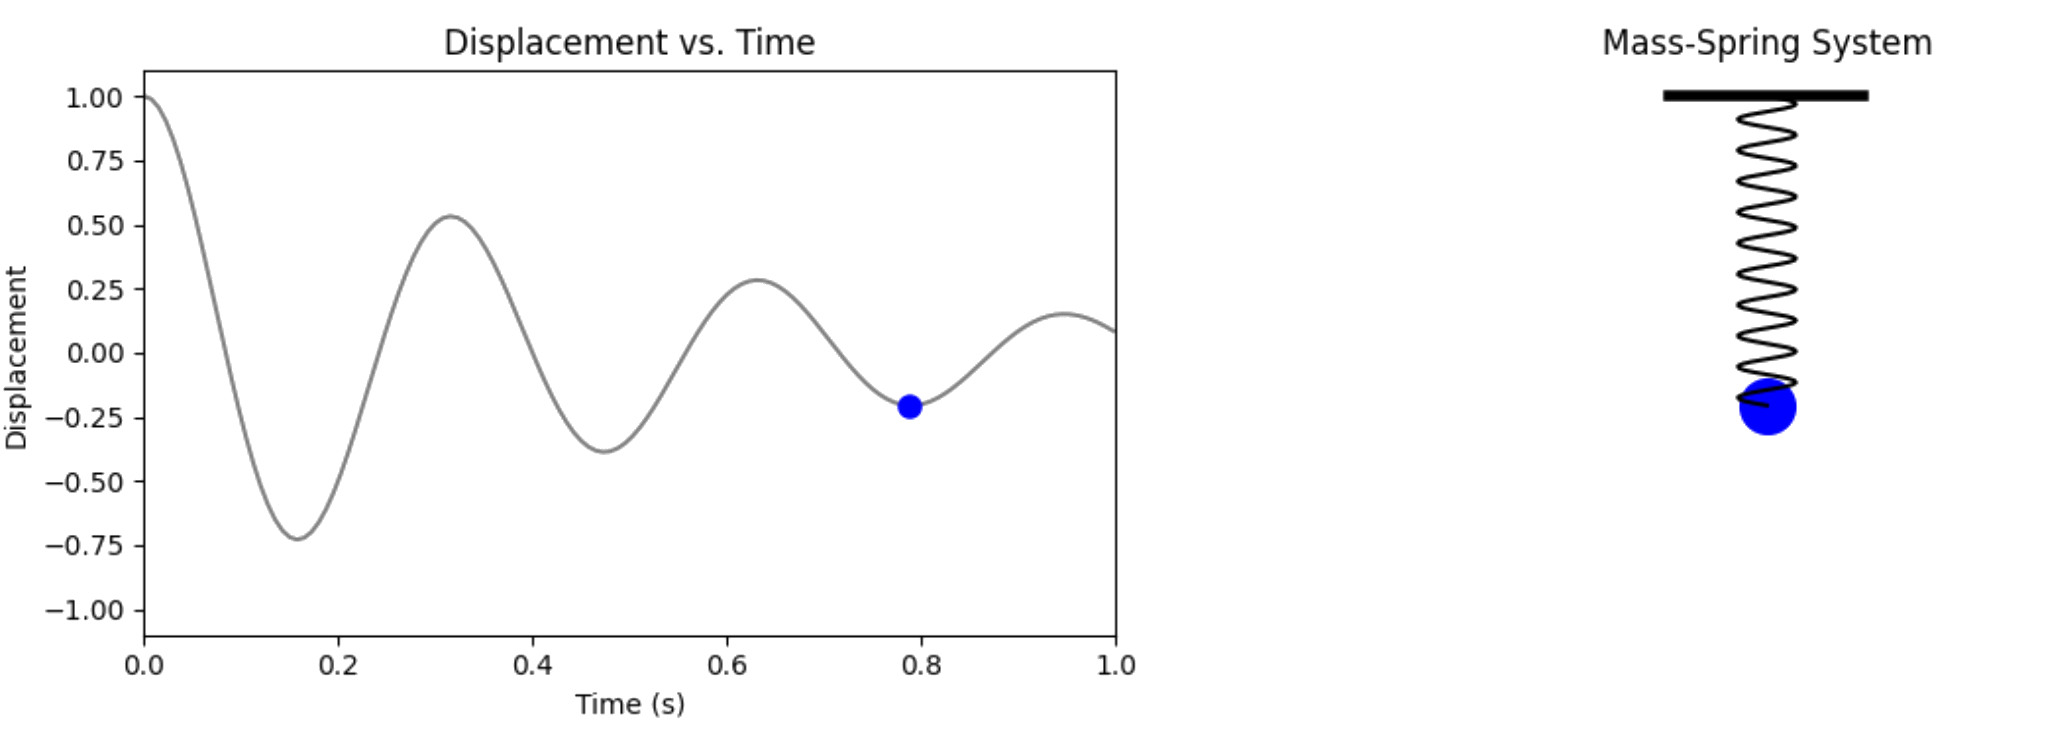
\includegraphics[width=0.75\linewidth]{chapters/04-pinns/figs/harmonic-oscillator.png}
    \caption{Harmonic oscillation of an underdamped system.}
    \label{fig:harmonic_oscillator} % Consistent label
\end{figure}

Now, suppose we have performed an experiment and measured the displacement $u$ only at a few discrete times $t_1, t_2, \ldots, t_N$. Let's denote these measurements as $u_1, u_2, \ldots, u_N$. These data points might be sparse and could contain some experimental noise. Our goal is to find the function $u(t)$ that describes the system's behavior for all times $t$.

\notebook[Interactive Notebook: Harmonic Oscillator Example]{https://sciml-book.github.io/sciml_notebook/pinns/oscillator.html}

\subsection{Attempt 1: Using a Standard Neural Network (Data-Driven Approach)}

Neural networks are powerful function approximators. A natural first thought is: can we train a neural network to learn the relationship between time $t$ and displacement $u(t)$ directly from our measured data points $(t_i, u_i)$?

Let's represent the neural network's approximation of the displacement as $\hat{u}_\theta(t)$, where $\theta$ represents all the trainable parameters (weights and biases) of the network. A typical feedforward network architecture might consist of an input layer (taking time $t$), a few hidden layers with activation functions (like $\tanh$), and an output layer producing the predicted displacement $\hat{u}_\theta$, as shown in \cref{fig:oscillator_nn_arch}.

\begin{figure}[htbp]
    \centering
    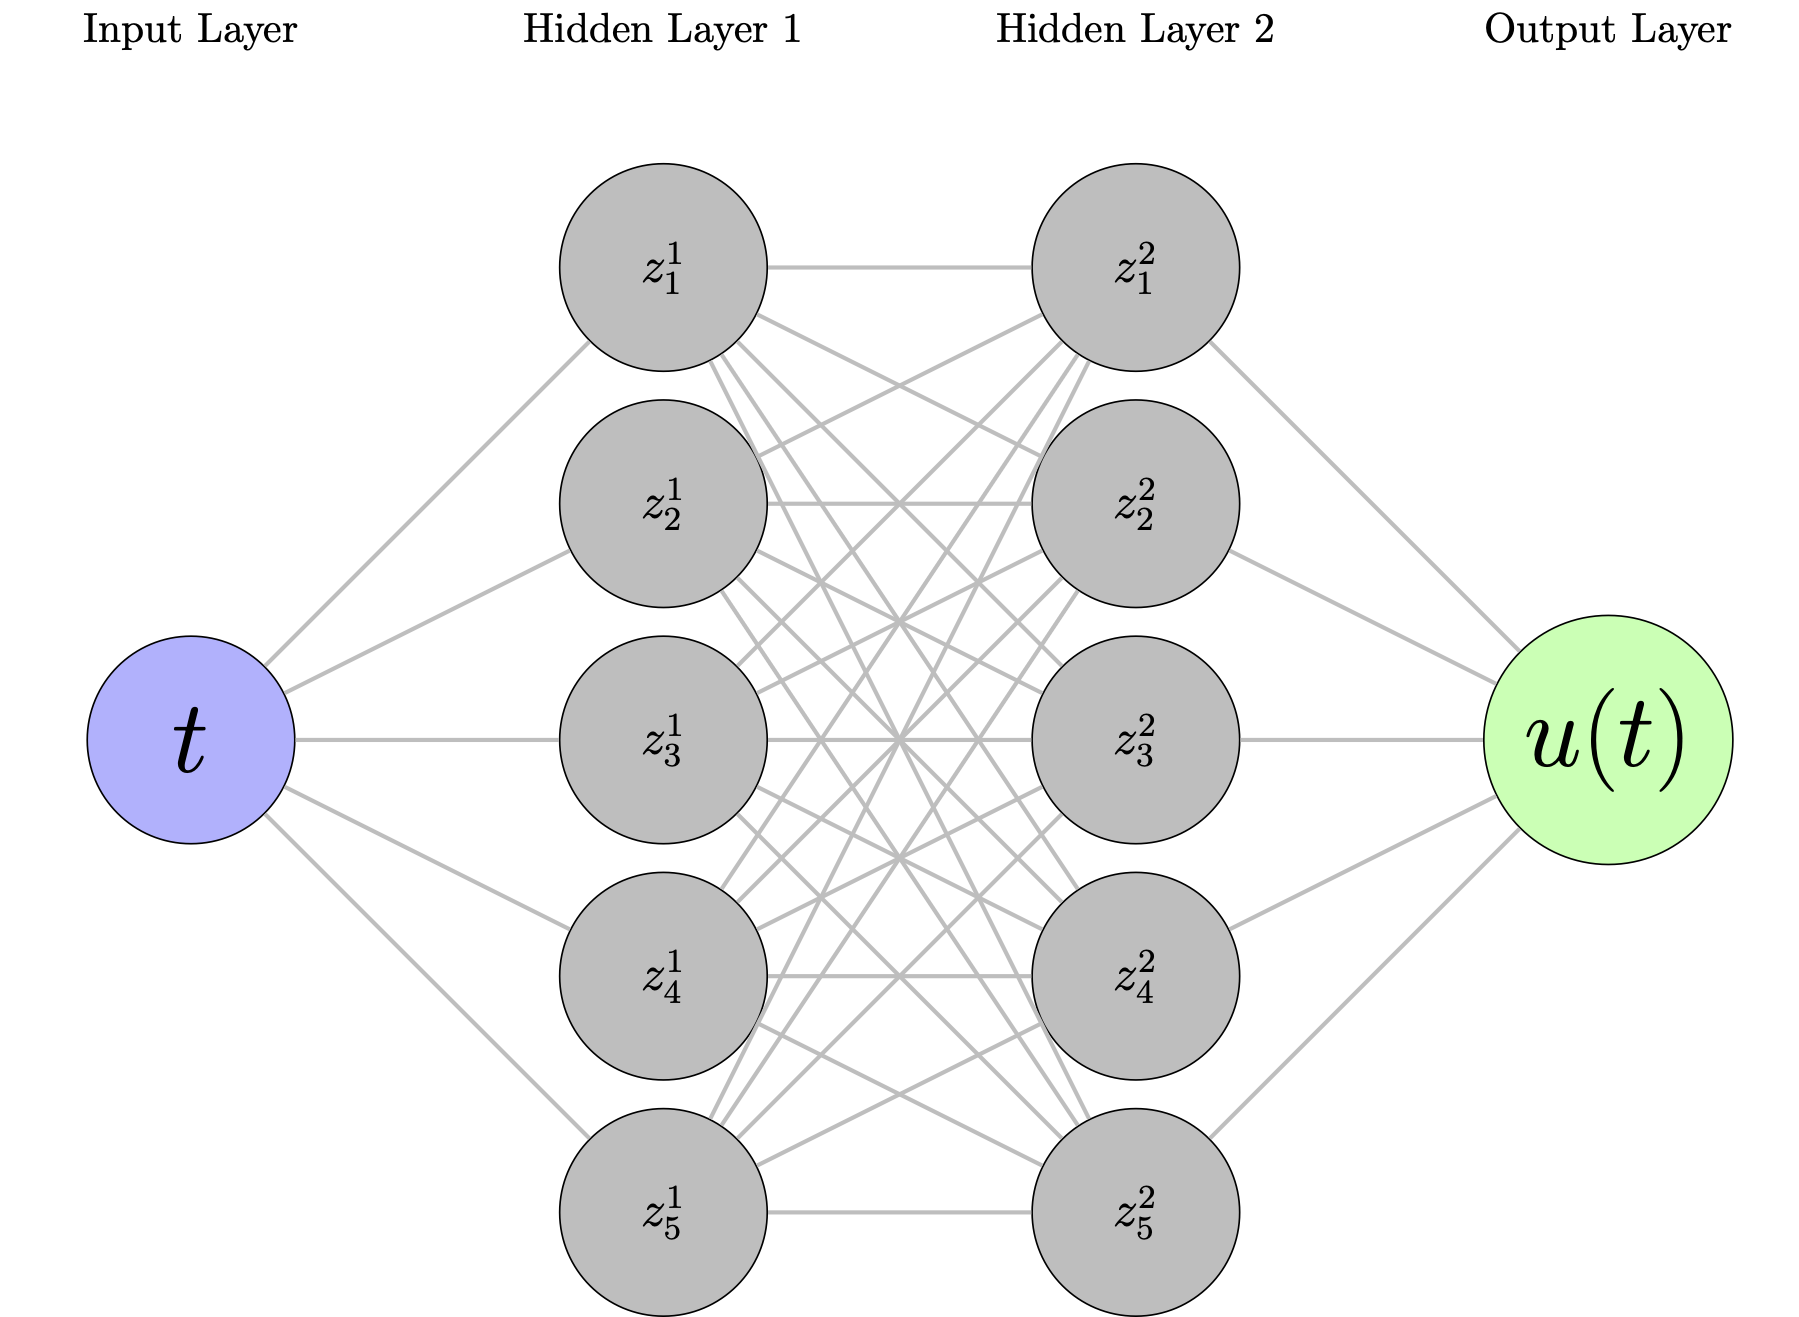
\includegraphics[width=0.7\textwidth]{chapters/04-pinns/figs/oscillator-nn.pdf}
    \caption{A standard feedforward neural network architecture used to approximate the oscillator's displacement $u(t)$ from input time $t$.}
    \label{fig:oscillator_nn_arch} % Consistent label
\end{figure}

How do we train this network? We need a way to measure how well its predictions match the data. We define a \textbf{loss function}, typically the mean squared error (MSE) between the network's predictions at the measurement times $t_i$ and the actual measurements $u_i$:
%
\begin{equation}
\mathcal{L}_{\text{data}}(\theta) = \frac{1}{N}\sum_{i=1}^N |\hat{u}_\theta(t_i) - u_i|^2\,.
\label{eq:loss_data}
\end{equation}
%
The goal of training is to find the network parameters $\theta$ that minimize this loss function. We use optimization algorithms, like gradient descent or its variants (e.g., Adam), which iteratively adjust $\theta$ based on the gradient of the loss:
%
\begin{equation*}
\theta_{k+1} = \theta_k - \eta \cdot \nabla_\theta \mathcal{L}_{\text{data}}(\theta_k)\,,
\end{equation*}
%
where $k$ is the iteration number and $\eta$ is the learning rate.

Does this data-driven approach work? Let's look at the results in \cref{fig:oscillator_result_nn}.

\begin{figure}[htbp]
    \centering
    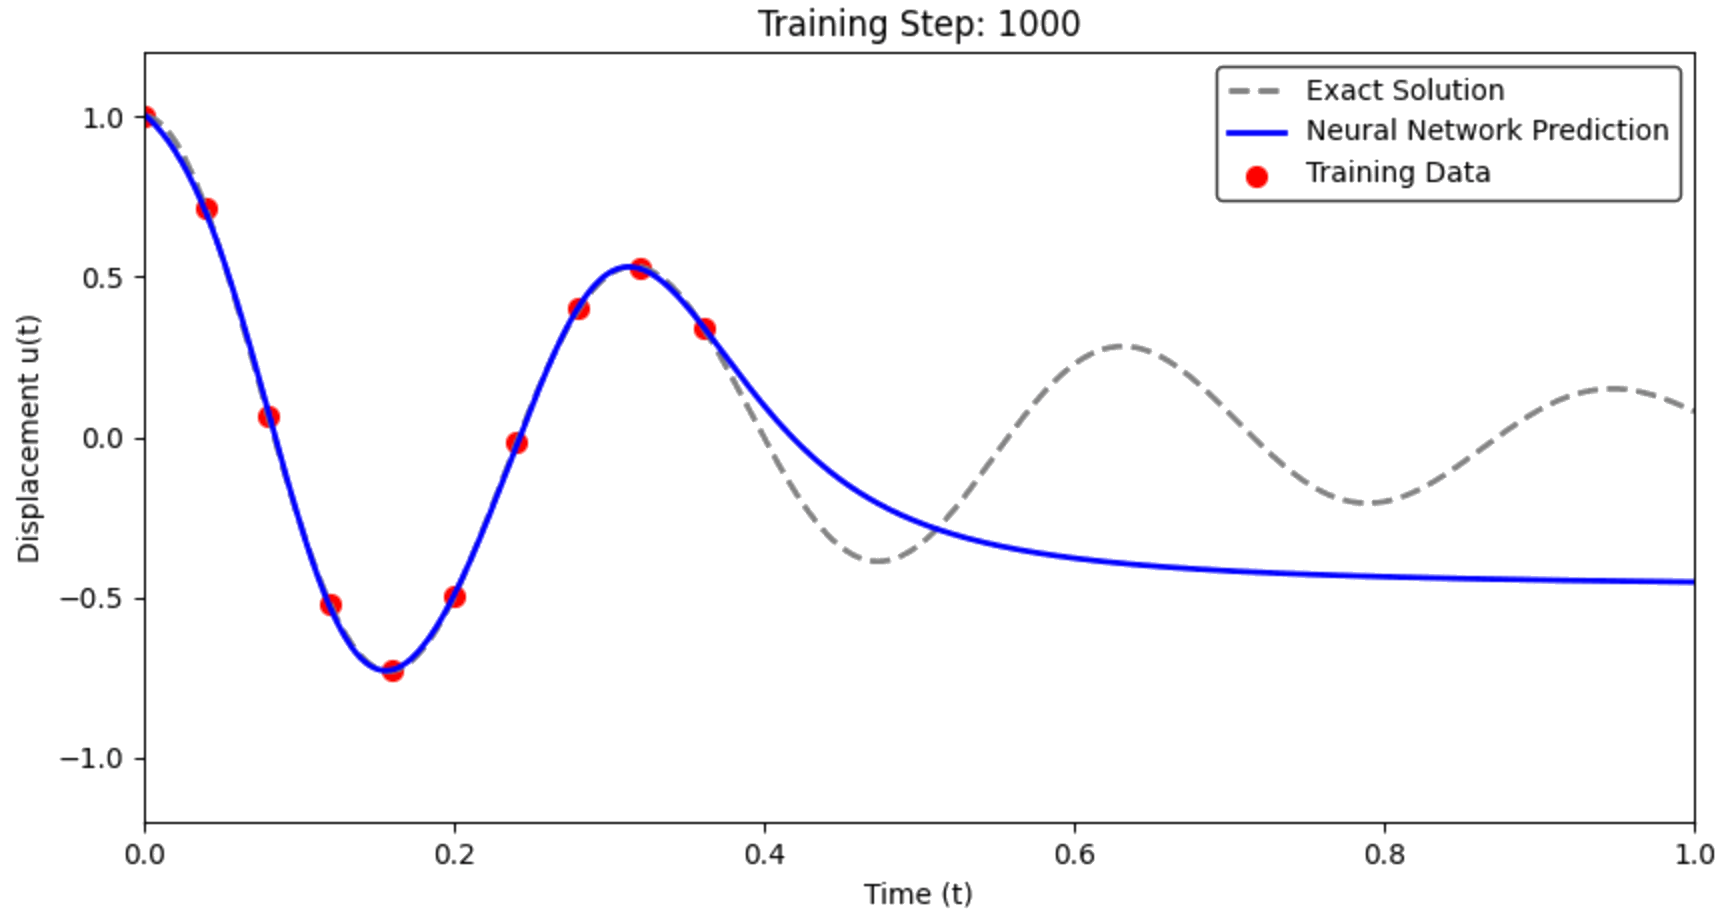
\includegraphics[width=0.75\linewidth]{chapters/04-pinns/figs/oscillator-result-nn.png}
    \caption{Prediction of the harmonic oscillator using a standard neural network trained only on sparse data points (red dots). While it fits the data points well, the prediction between points (blue dashed line) deviates significantly from the true solution (solid blue line).}
    \label{fig:oscillator_result_nn}
\end{figure}

The network (blue dashed line) learns to pass through or near the training data points (red dots). However, in the regions *between* these points, the network's prediction can deviate significantly from the true physical behavior (solid blue line). The network has simply learned to connect the dots in some way, without any understanding of the underlying physics governed by \cref{eq:oscillator_ode}. This approach fails to generalize well and may produce physically unrealistic results.

\subsection{Attempt 2: Incorporating Physics (The PINN Approach)}

The failure of the purely data-driven approach highlights a crucial missing piece: the physical law governing the system. Physics-Informed Neural Networks (PINNs), pioneered by Raissi et al.~\cite{raissi2019physics}, address this by integrating the physical laws directly into the learning process.

The core idea is elegant: we modify the loss function to penalize the network not only for mismatching the data but also for violating the differential equation.

First, let's define the \textbf{residual} of the differential equation when the neural network solution $\hat{u}_\theta(t)$ is plugged in:
%
\begin{equation}
\mathcal{R}_\theta(t) = m\frac{d^2\hat{u}_\theta}{dt^2}(t) + c\frac{d\hat{u}_\theta}{dt}(t) + k\hat{u}_\theta(t)\,.
\label{eq:residual_oscillator}
\end{equation}
%
If $\hat{u}_\theta$ were the exact solution to \cref{eq:oscillator_ode}, this residual $\mathcal{R}_\theta (t)$ would be exactly zero for all $t$. For our network approximation, we want this residual to be as close to zero as possible, not just at the data points, but *everywhere* in the time domain of interest.

How do we enforce this? We introduce a set of points, $\{t_j^c\}_{j=1}^{N_c}$, called \textbf{collocation points}, distributed throughout the time domain (e.g., uniformly spaced or randomly sampled). These points are specifically chosen to evaluate how well the network satisfies the physics. They do not need to coincide with the data points $\{t_i\}$.

At each collocation point $t_j^c$, we compute the residual $\mathcal{R}_\theta(t_j^c)$. We then define the \textbf{physics loss} as the mean squared error of these residuals:
%
\begin{equation}
\mathcal{L}_{\text{physics}}(\theta) = \frac{1}{N_c}\sum_{j=1}^{N_c}|\mathcal{R}_\theta(t_j^c)|^2\,.
\label{eq:loss_physics}
\end{equation}
%
This term will be small only if the neural network $\hat{u}_\theta(t)$ approximately satisfies the differential equation \eqref{eq:oscillator_ode} at all the collocation points.

The total loss function for the PINN now combines the data fidelity term and the physics enforcement term:
%
\begin{equation}
\mathcal{L}_{\text{total}}(\theta) = \mathcal{L}_{\text{data}}(\theta) + \lambda\mathcal{L}_{\text{physics}}(\theta) \,,
\label{eq:loss_total_pinn}
\end{equation}
%
where $\mathcal{L}_{\text{data}}$ is given by \cref{eq:loss_data}, $\mathcal{L}_{\text{physics}}$ by \cref{eq:loss_physics}, and $\lambda$ is a positive weighting parameter. This hyperparameter $\lambda$ balances the importance between fitting the observed data and satisfying the physical law. A careful choice of $\lambda$ can be important, though often a fixed value (e.g., $\lambda = 10^{-4}$ was used in the original example) works well, or adaptive methods can be used (see \cref{sec:weight-selection}).

By minimizing $\mathcal{L}_{\text{total}}(\theta)$, the network is trained to simultaneously:
\begin{enumerate}
    \item Match the observed data points $(t_i, u_i)$.
    \item Satisfy the governing differential equation \eqref{eq:oscillator_ode} at the collocation points $t_j^c$.
\end{enumerate}

\subsection{Computing Derivatives: The Role of Automatic Differentiation}

A critical question arises: how do we compute the derivatives $\frac{d\hat{u}_\theta}{dt}$ and $\frac{d^2\hat{u}_\theta}{dt^2}$ needed for the residual $\mathcal{R}_\theta(t)$ in \cref{eq:residual_oscillator}?

Using numerical approximations like finite differences would introduce errors and potentially instability. Fortunately, modern deep learning frameworks provide a powerful tool: \textbf{Automatic Differentiation (AD)}.

AD is a set of techniques to computationally evaluate the derivative of a function specified by a computer program. Crucially, AD computes derivatives *exactly* (up to machine precision), not numerically. It works by systematically applying the chain rule of calculus at the elementary operation level within the network's computation graph.

For our neural network $\hat{u}_\theta(t)$, AD allows us to compute the exact derivatives with respect to the input $t$:
%
\begin{align*}
\frac{d\hat{u}_\theta}{dt}(t) &= \nabla_t \hat{u}_\theta(t) \\
\frac{d^2\hat{u}_\theta}{dt^2}(t) &= \nabla_t \left(\nabla_t \hat{u}_\theta(t)\right)
\end{align*}
%
Here, $\nabla_t$ represents the differentiation operation performed by AD. It's important to remember that these are the exact derivatives *of the function represented by the neural network*, which is itself an approximation to the true solution $u(t)$.

The availability of AD is a key reason why PINNs have become practical. It allows us to incorporate differential operators into the loss function accurately and efficiently, enabling the network to learn functions that respect the underlying physics. (For more details on AD, see Chapter X - \textit{placeholder for AD chapter reference}).

\subsection{The Harmonic Oscillator Solved with a PINN}

Let's revisit the harmonic oscillator, now using the PINN approach. The setup involves:
\begin{itemize}
    \item A neural network $\hat{u}_\theta(t)$ approximating the displacement.
    \item A loss function $\mathcal{L}_{\text{total}} = \mathcal{L}_{\text{data}} + \lambda\mathcal{L}_{\text{physics}}$.
    \item $\mathcal{L}_{\text{data}}$ measures mismatch with measurements $(t_i, u_i)$.
    \item $\mathcal{L}_{\text{physics}}$ measures the residual \eqref{eq:residual_oscillator} at collocation points $t_j^c$, using derivatives computed via AD.
    \item An optimizer minimizes $\mathcal{L}_{\text{total}}$ to find the best parameters $\theta$.
\end{itemize}
The architecture, illustrated in \cref{fig:oscillator_pinn_nn}, now explicitly includes the computation of the physics residual using AD.

\begin{figure}[htbp]
    \centering
    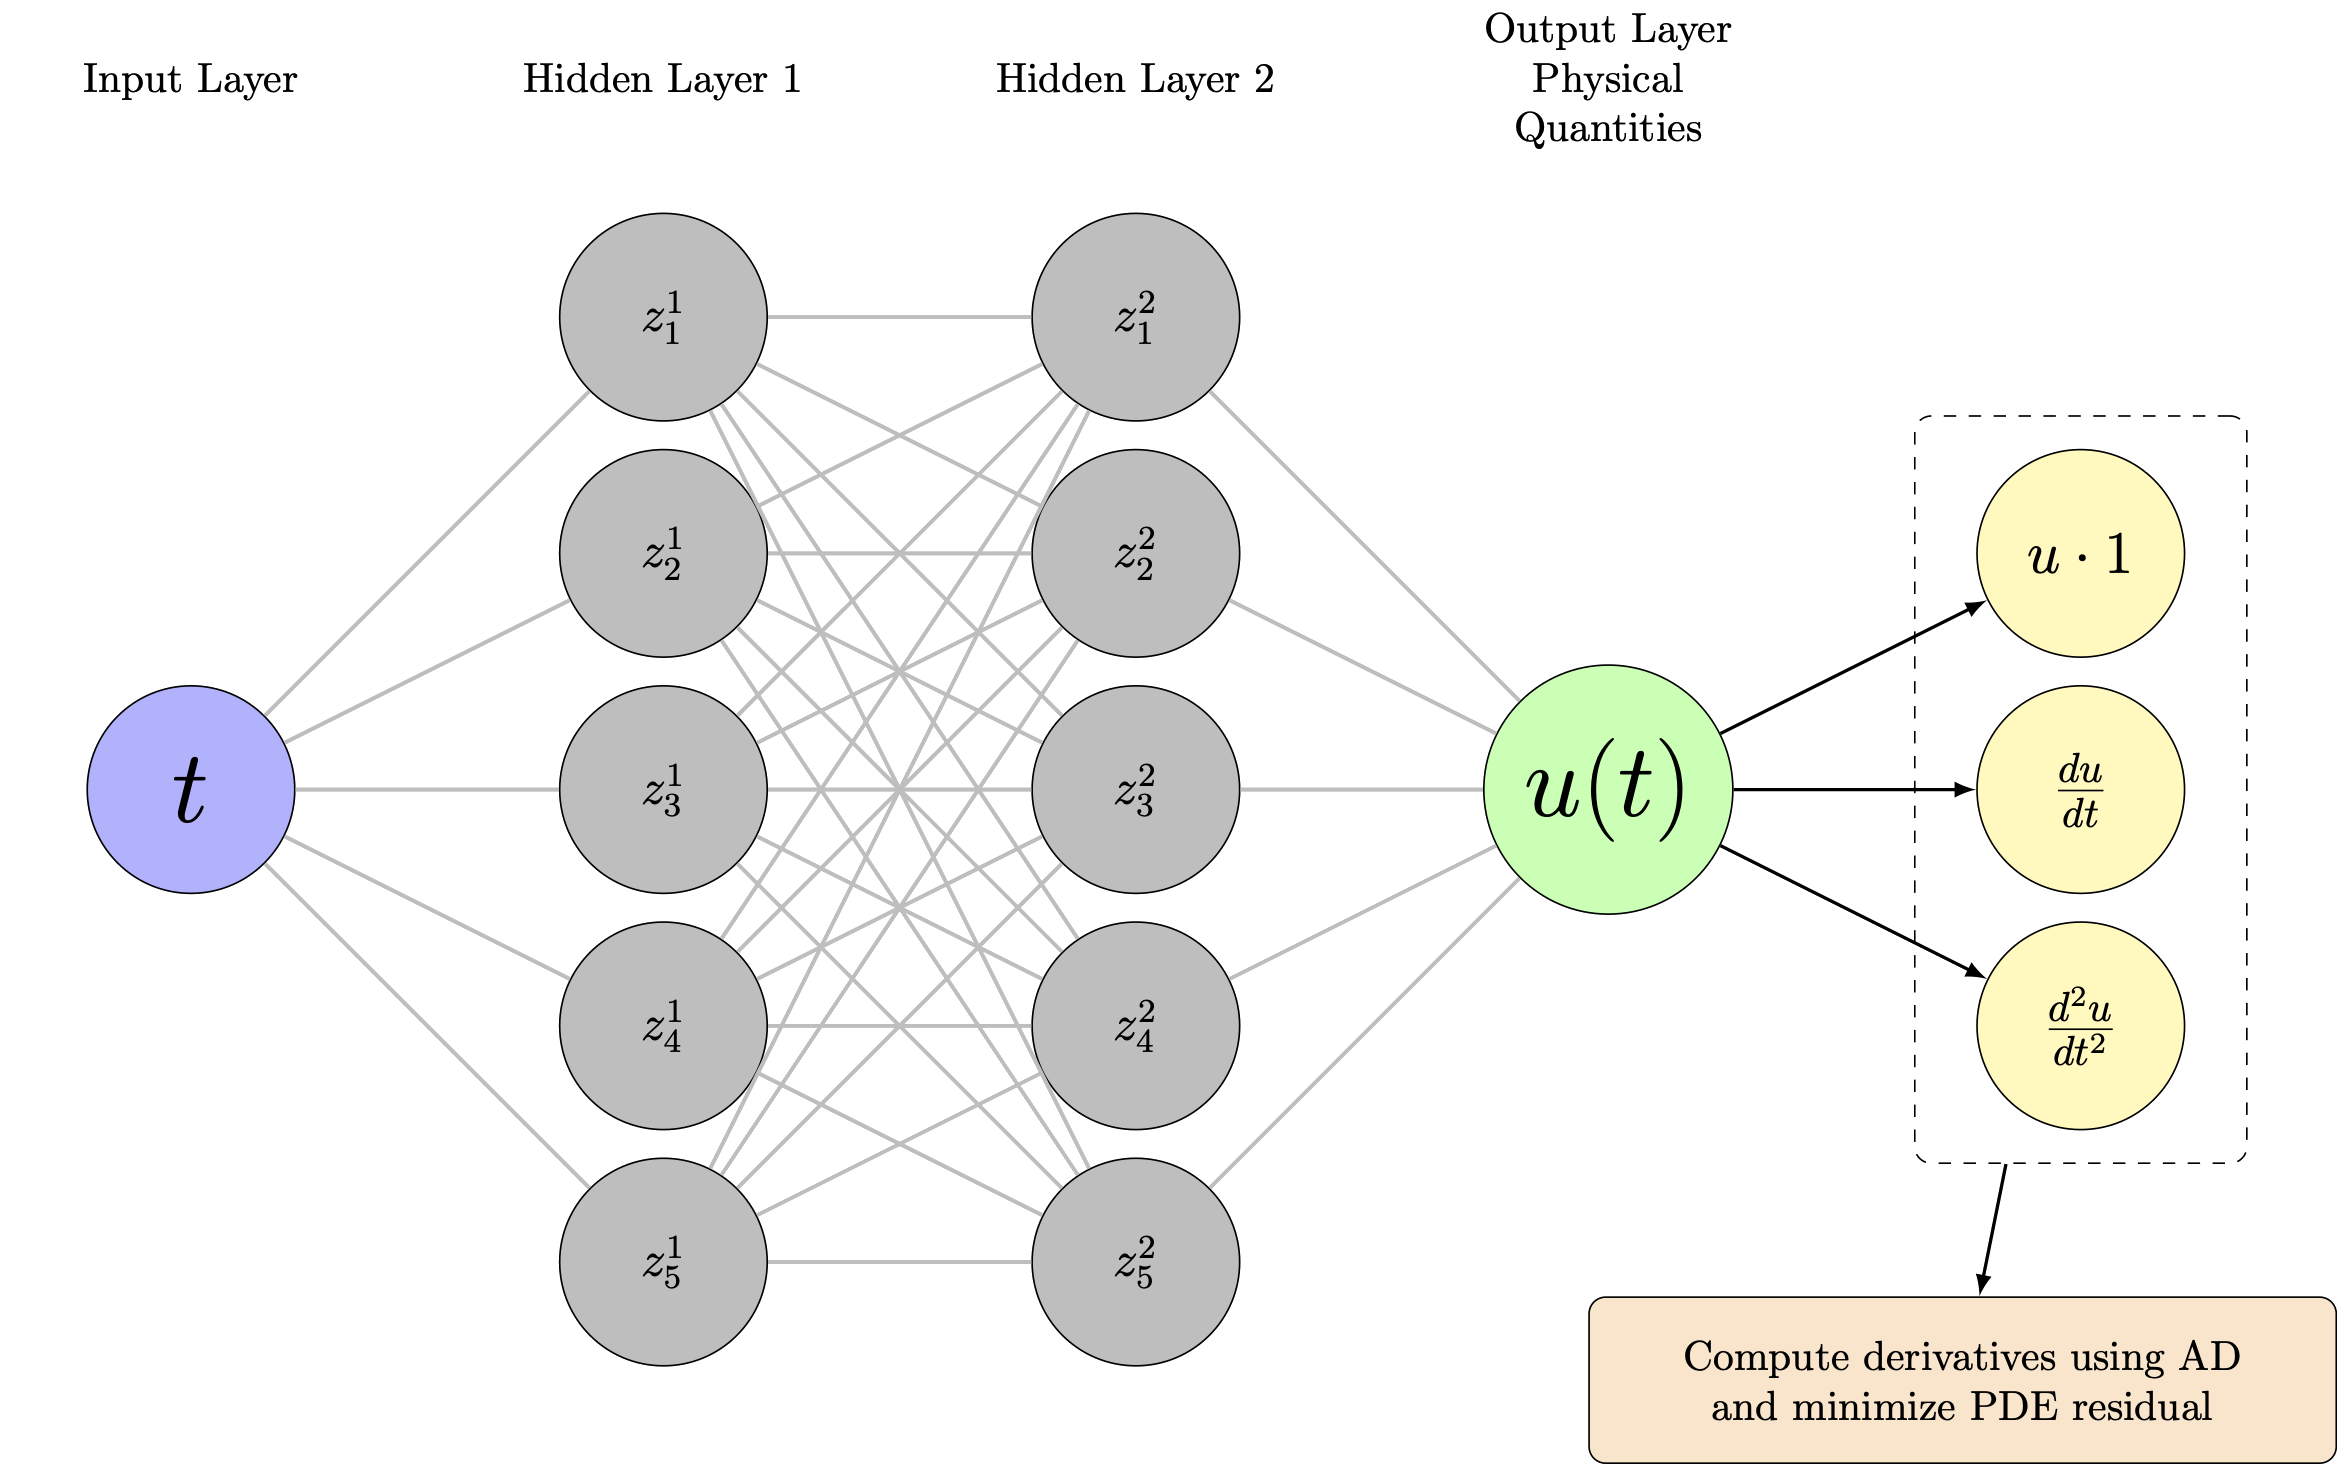
\includegraphics[width=\textwidth]{chapters/04-pinns/figs/oscillator-pinn-nn.pdf}
    \caption{Physics-informed neural network (PINN) model for the oscillator. The network predicts $\hat{u}_\theta(t)$. Automatic differentiation computes $d\hat{u}_\theta/dt$ and $d^2\hat{u}_\theta/dt^2$, which are used to calculate the physics residual $\mathcal{R}(t)$. The total loss combines data mismatch and the physics residual.}
    \label{fig:oscillator_pinn_nn}
\end{figure}

\Cref{fig:oscillator_result_pinn} shows the prediction obtained from the trained PINN.

\begin{figure}[htbp]
    \centering
    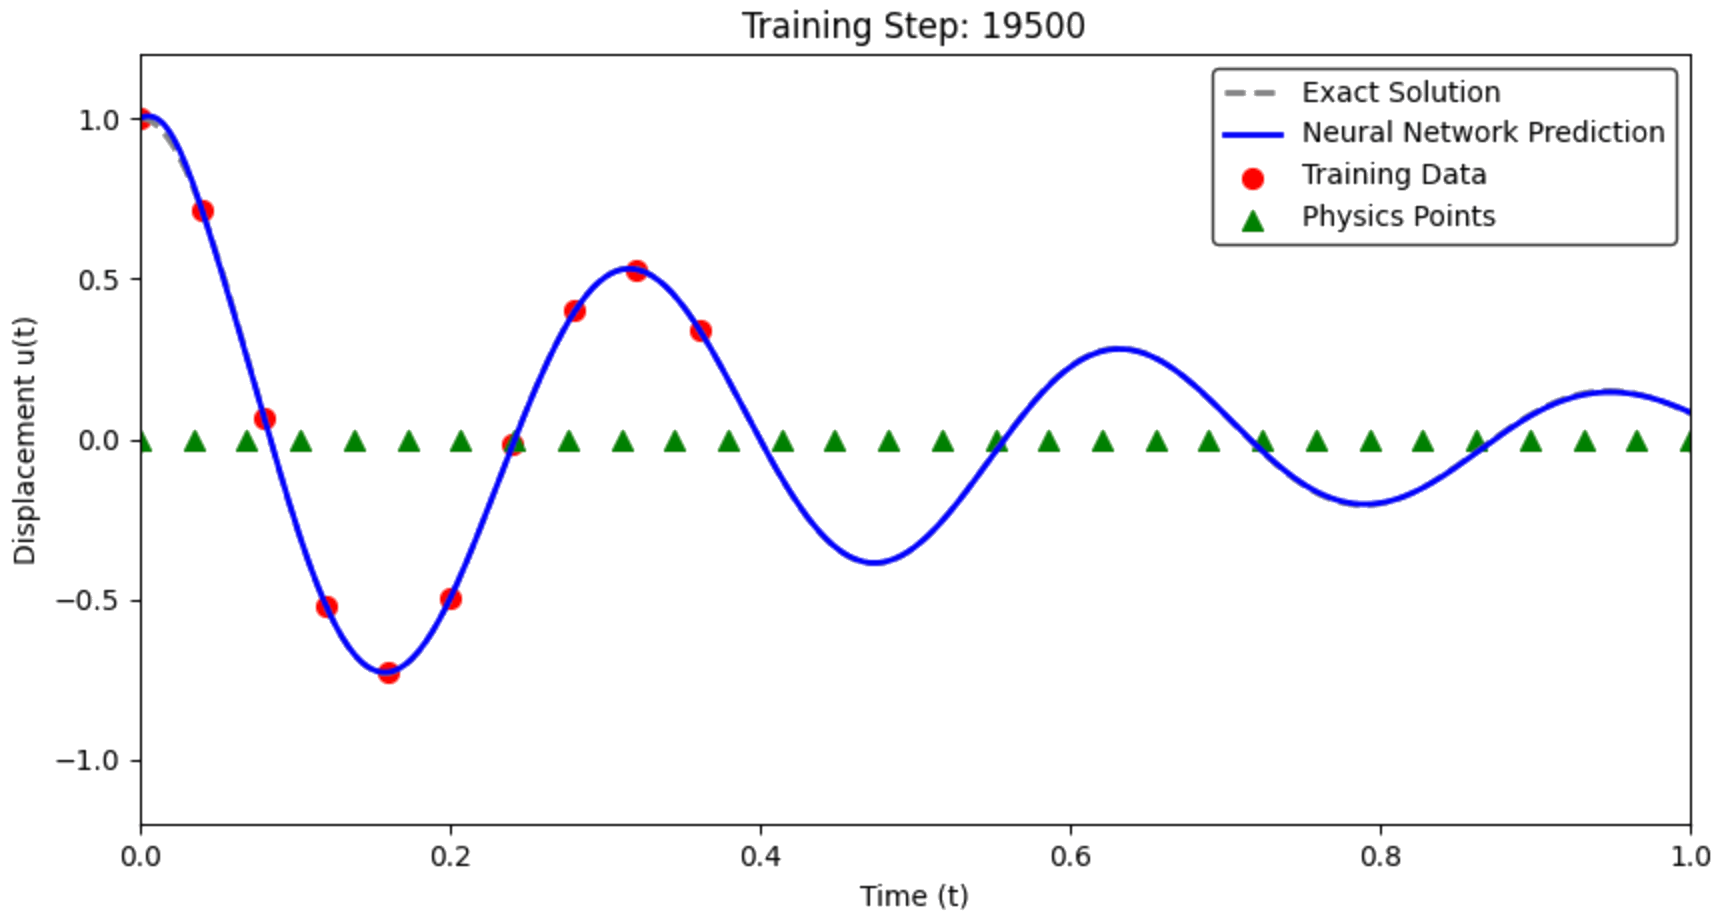
\includegraphics[width=0.75\linewidth]{chapters/04-pinns/figs/oscillator-result-pinn.png}
    \caption{PINN prediction of the harmonic oscillator (blue curve) compared to the exact solution (dashed green line) and training data (red dots). The physics constraint enables accurate generalization far from the training points.}
    \label{fig:oscillator_result_pinn}
\end{figure}

The result is striking. The PINN solution (blue curve) not only fits the sparse training data (red dots) but also accurately follows the true solution (dashed green line) across the entire domain. Compare this success with the failure of the data-only network shown in \cref{fig:oscillator_result_nn}.

The inclusion of the $\mathcal{L}_{\text{physics}}$ term acts as a powerful \textbf{regularizer}. It constrains the space of possible functions the network can learn, guiding it towards solutions that are physically plausible and preventing the overfitting seen in the purely data-driven approach. This ability to embed physical laws, leveraging the power of neural networks and automatic differentiation, is the core strength of PINNs.

\begin{criticalreflection}
\begin{itemize}
    \item If we had an extremely dense set of perfectly accurate data points covering the entire time domain, would this ``physics-agnostic" NN likely produce a physically plausible solution for the oscillator? Why might it still be less desirable than an approach that explicitly uses the ODE?
\end{itemize}

\end{criticalreflection}

\subsection{Generalizing the PINN Concept}

While we used the simple harmonic oscillator (an ODE) to illustrate the core concepts, the PINN approach is broadly applicable to various types of partial differential equations (PDEs) involving multiple independent variables (e.g., time and space).

For a general PDE system involving a function $u(x,t)$ and a differential operator $\mathcal{N}$, potentially with parameters $\lambda$:
\begin{equation*}
\frac{\partial u}{\partial t} + \mathcal{N}[u; \lambda] = 0, \quad \text{in domain } \Omega \times [0,T]
\end{equation*}
along with appropriate initial and boundary conditions, the PINN framework remains similar:
\begin{enumerate}
    \item Approximate the solution $u(x,t)$ with a neural network $\hat{u}_\theta(x,t)$.
    \item Define a loss function including terms for:
        \begin{itemize}
            \item Initial conditions (data at $t=0$).
            \item Boundary conditions (data or constraints on $\partial\Omega$).
            \item PDE residual (evaluated at collocation points $(x_j^c, t_j^c)$ within $\Omega \times [0,T]$ using AD for derivatives).
        \end{itemize}
    \item Train the network by minimizing the total loss.
\end{enumerate}

This framework can handle complex, nonlinear PDEs and offers flexibility in incorporating different types of boundary conditions (discussed in \cref{sec:weak_bc,sec:strong_bc}) and even solving inverse problems where parameters like $\lambda$ are unknown (see \cref{sec:inverse_problems}). In the following sections, we will explore these aspects, along with the underlying mathematical foundations and practical considerations.

\section{The PINN Framework: Generalizing the Approach}
\label{sec:pinn_framework}

The damped harmonic oscillator example illustrated the core idea of PINNs: combining data fitting with physics enforcement through a modified loss function.
Now, let's generalize this framework to handle a broader class of problems governed by partial differential equations (PDEs).

Consider a general physical system described by a function $u(\mathbf{x})$, where $\mathbf{x}$ represents the independent variables (e.g., space $\mathbf{x}=(x,y,z)$ and/or time $t$). The system's behavior is governed by a differential equation within a domain $\Omega$:
%
\begin{equation}
\mathcal{N}[u](\mathbf{x}) = f(\mathbf{x}), \quad \mathbf{x} \in \Omega \,,
\label{eq:pde_general}
\end{equation}
%
where $\mathcal{N}$ is a differential operator (which can be linear or nonlinear, involving various partial derivatives of $u$), and $f(\mathbf{x})$ is a known source term.

Furthermore, the solution $u(\mathbf{x})$ must satisfy specific conditions on the domain boundary, $\partial\Omega$. These are represented by a boundary operator $\mathcal{B}$:
%
\begin{equation}
\mathcal{B}[u](\mathbf{x}) = g(\mathbf{x}), \quad \mathbf{x} \in \partial\Omega \,,
\label{eq:bc_general}
\end{equation}
%
where $g(\mathbf{x})$ represents the prescribed boundary values or conditions (e.g., Dirichlet, Neumann, or Robin conditions). 
For time-dependent problems, initial conditions at $t=0$ would also be specified.

\subsection{Approximating the Solution with a Neural Network}

The central idea of PINNs is to approximate the unknown solution $u(\mathbf{x})$ using a neural network, which we denote as $\hat{u}_\theta(\mathbf{x}; \boldsymbol{\theta})$. 
Here, $\boldsymbol{\theta}$ represents the collection of all trainable parameters (weights and biases) within the network. A standard feedforward neural network architecture is typically used:
%
\begin{equation*}
\hat{u}_\theta(\mathbf{x}; \boldsymbol{\theta}) = \text{OutputLayer}(\dots \text{HiddenLayer}_2(\text{HiddenLayer}_1(\mathbf{x}; \boldsymbol{\theta}_1)); \dots ; \boldsymbol{\theta}_L)\,.
\end{equation*}
%
The network takes the coordinates $\mathbf{x}$ as input and, after processing through $L$ layers with activation functions $\sigma$, outputs an approximation to the solution $u(\mathbf{x})$. The goal of training is to find the optimal parameters $\boldsymbol{\theta}$ such that $\hat{u}_\theta(\mathbf{x}; \boldsymbol{\theta})$ closely approximates the true solution $u(\mathbf{x})$.

\subsection{The Physics-Informed Loss Function}

Unlike standard supervised learning where the loss function only measures the mismatch with known data points, the PINN loss function incorporates terms that enforce the physical laws described by the PDE and boundary conditions. The total loss $\mathcal{L}(\boldsymbol{\theta})$ is typically a weighted sum of several components:

\begin{equation}
\mathcal{L}(\boldsymbol{\theta}) = w_{\text{PDE}}\mathcal{L}_{\text{PDE}}(\boldsymbol{\theta}) + w_{\text{BC}}\mathcal{L}_{\text{BC}}(\boldsymbol{\theta}) + w_{\text{IC}}\mathcal{L}_{\text{IC}}(\boldsymbol{\theta}) + w_{\text{data}}\mathcal{L}_{\text{data}}(\boldsymbol{\theta}) \,.
\label{eq:loss_general}
\end{equation}
%
Let's break down each component:

\begin{enumerate}
    \item \textbf{PDE Residual Loss ($\mathcal{L}_{\text{PDE}}$):} This term enforces the governing differential equation \eqref{eq:pde_general}. We define the PDE residual using the network approximation:
    %
    \begin{equation*}
    \mathcal{R}_{\text{PDE}}(\mathbf{x}; \boldsymbol{\theta}) = \mathcal{N}[\hat{u}_\theta](\mathbf{x}; \boldsymbol{\theta}) - f(\mathbf{x})\,.
    \end{equation*}
    %
    This residual should ideally be zero everywhere in the domain $\Omega$. We enforce this by sampling a set of $N_f$ \textbf{collocation points} $\{\mathbf{x}_i^f\}_{i=1}^{N_f}$ inside the domain $\Omega$ and minimizing the mean squared residual:
    %
    \begin{equation}
    \mathcal{L}_{\text{PDE}}(\boldsymbol{\theta}) = \frac{1}{N_{f}} \sum_{i=1}^{N_{f}} \left| \mathcal{R}_{\text{PDE}}(\mathbf{x}_i^f; \boldsymbol{\theta}) \right|^2\,.
    \label{eq:pde_loss_general}
    \end{equation}
    Crucially, computing the operator $\mathcal{N}[\hat{u}_\theta]$ requires calculating derivatives of the network's output with respect to its inputs, which is done using Automatic Differentiation (AD).

    \item \textbf{Boundary Condition Loss ($\mathcal{L}_{\text{BC}}$):} This term enforces the boundary conditions \eqref{eq:bc_general}. We define the boundary residual:
    %
    \begin{equation*}
    \mathcal{R}_{\text{BC}}(\mathbf{x}; \boldsymbol{\theta}) = \mathcal{B}[\hat{u}_\theta](\mathbf{x}; \boldsymbol{\theta}) - g(\mathbf{x})\,.
    \end{equation*}
    %
    We sample $N_b$ points $\{\mathbf{x}_j^b\}_{j=1}^{N_b}$ on the boundary $\partial\Omega$ and minimize the mean squared boundary residual:
    %
    \begin{equation}
    \mathcal{L}_{\text{BC}}(\boldsymbol{\theta}) = \frac{1}{N_{b}} \sum_{j=1}^{N_{b}} \left| \mathcal{R}_{\text{BC}}(\mathbf{x}_j^b; \boldsymbol{\theta}) \right|^2\,.
    \label{eq:bc_loss_general}
    \end{equation}
    Again, AD is used if the boundary operator $\mathcal{B}$ involves derivatives (like in Neumann conditions).

    \item \textbf{Initial Condition Loss ($\mathcal{L}_{\text{IC}}$):} For time-dependent problems, we need to enforce the initial condition, typically $u(\mathbf{x}, 0) = u_0(\mathbf{x})$. We sample $N_{ic}$ points $\{\mathbf{x}_k^{ic}\}_{k=1}^{N_{ic}}$ within the spatial domain at $t=0$ and define:
    %
    \begin{equation}
    \mathcal{L}_{\text{IC}}(\boldsymbol{\theta}) = \frac{1}{N_{ic}} \sum_{k=1}^{N_{ic}} \left| \hat{u}_\theta(\mathbf{x}_k^{ic}, 0; \boldsymbol{\theta}) - u_0(\mathbf{x}_k^{ic}) \right|^2\,.
    \label{eq:ic_loss_general}
    \end{equation}

    \item \textbf{Data Loss ($\mathcal{L}_{\text{data}}$):} If we have specific measurements $( \mathbf{x}_m^{data}, u_m^{data} )$ of the solution at $N_{data}$ points (like in our oscillator example), we can include a data fidelity term, similar to standard supervised learning:
    %
    \begin{equation}
    \mathcal{L}_{\text{data}}(\boldsymbol{\theta}) = \frac{1}{N_{data}} \sum_{m=1}^{N_{data}} \left| \hat{u}_\theta(\mathbf{x}_m^{data}; \boldsymbol{\theta}) - u_m^{data} \right|^2\,.
    \label{eq:data_loss_general}
    \end{equation}
    This term anchors the solution to known values. In many PINN applications, especially for forward problems where the equation is fully defined, this term might be absent ($w_{data}=0$).
\end{enumerate}

The weights $w_{\text{PDE}}, w_{\text{BC}}, w_{\text{IC}}, w_{\text{data}}$ in \cref{eq:loss_general} are hyperparameters that balance the contribution of each loss component. Their selection can significantly impact training performance and accuracy (see \cref{sec:weight-selection}).

\subsection{Training the Network}

The training process aims to find the optimal network parameters $\boldsymbol{\theta}^*$ that minimize the total loss function $\mathcal{L}(\boldsymbol{\theta})$. This is typically achieved using gradient-based optimization algorithms like Adam or L-BFGS. The core steps involve:
%
\begin{enumerate}
    \item Initialize the network parameters $\boldsymbol{\theta}$.
    \item Iteratively:
        \begin{itemize}
            \item Sample collocation points (and data points, if applicable).
            \item Compute each component of the loss function ($\mathcal{L}_{\text{PDE}}, \mathcal{L}_{\text{BC}}, \dots$), using AD to evaluate necessary derivatives within the residuals.
            \item Compute the total loss $\mathcal{L}(\boldsymbol{\theta})$.
            \item Compute the gradient of the total loss with respect to the parameters, $\nabla_{\boldsymbol{\theta}} \mathcal{L}(\boldsymbol{\theta})$, typically via backpropagation (which itself relies on AD).
            \item Update the parameters $\boldsymbol{\theta}$ using the optimizer's rule (e.g., $\boldsymbol{\theta}_{k+1} = \boldsymbol{\theta}_k - \eta \nabla_{\boldsymbol{\theta}} \mathcal{L}(\boldsymbol{\theta}_k)$).
        \end{itemize}
    \item Continue until a convergence criterion is met (e.g., loss falls below a threshold, or a maximum number of iterations is reached).
\end{enumerate}
%
A schematic of the training algorithm is shown in Algorithm~\ref{alg:training_general} (note: this is a conceptual outline; practical implementations often use minibatches).

\begin{algorithm}[H] % Using algorithm package
\caption{Conceptual Training Algorithm for PINNs}
\label{alg:training_general}
\KwIn{Network architecture, PDE/BC definitions, hyperparameters (learning rate $\eta$, weights $w$, etc.)}
\KwOut{Trained network parameters $\boldsymbol{\theta}^*$}

Initialize $\boldsymbol{\theta}$ randomly\;
\While{not converged}{
    Sample points: $\{\mathbf{x}_i^f\}$, $\{\mathbf{x}_j^b\}$, $\{\mathbf{x}_k^{ic}\}$, $\{\mathbf{x}_m^{data}\}$\;
    Compute residuals $\mathcal{R}_{\text{PDE}}$, $\mathcal{R}_{\text{BC}}$ using $\hat{u}_\theta(\cdot; \boldsymbol{\theta})$ and AD\;
    Compute loss components $\mathcal{L}_{\text{PDE}}, \mathcal{L}_{\text{BC}}, \mathcal{L}_{\text{IC}}, \mathcal{L}_{\text{data}}$\;
    Compute total loss $\mathcal{L}(\boldsymbol{\theta})$ using \cref{eq:loss_general}\;
    Compute gradient $\nabla_{\boldsymbol{\theta}} \mathcal{L}(\boldsymbol{\theta})$ via backpropagation\;
    Update $\boldsymbol{\theta} \leftarrow \boldsymbol{\theta} - \eta \nabla_{\boldsymbol{\theta}} \mathcal{L}(\boldsymbol{\theta})$\;
}
\Return $\boldsymbol{\theta}^*$
\end{algorithm}

\subsection{Relation to Least Squares Methods}

The PINN framework resembles classical least squares methods for solving PDEs. Both approaches aim to minimize the sum of squared residuals of the governing equations and boundary conditions evaluated at discrete points.
The fundamental difference lies in the choice of the approximating function. \textit{Classical Least Squares:} Approximates the solution $u(\mathbf{x})$ as a linear combination of predefined basis functions $\phi_k(\mathbf{x})$ (e.g., polynomials, splines): $u_{LS}(\mathbf{x}) = \sum_k c_k \phi_k(\mathbf{x})$. The goal is to find the optimal coefficients $c_k$. Derivatives are computed analytically or numerically from the basis functions. 
\textit{PINNs:} Approximates the solution $u(\mathbf{x})$ using a neural network $\hat{u}_\theta(\mathbf{x}; \boldsymbol{\theta})$. The ``basis functions" are implicitly defined by the network's architecture and activation functions. The goal is to find the optimal network parameters $\boldsymbol{\theta}$. Derivatives are computed exactly using Automatic Differentiation.
PINNs leverage the flexibility of neural networks as universal function approximators and the power of AD for derivative computation, allowing them to handle complex, nonlinear problems, often in higher dimensions, potentially more effectively than classical methods relying on fixed basis functions.

\subsection{Advantages of PINNs}
\begin{itemize}
    \item \textbf{Mesh-Free Formulation}: PINNs do not require mesh generation, simplifying the implementation for problems with complex or moving boundaries.

    \item \textbf{High Dimensionality Handling}: PINNs can efficiently handle high-dimensional PDEs, making them suitable for problems in finance, biology, and physics that involve multiple spatial and temporal dimensions.

    \item \textbf{Flexibility in Function Approximation}:  Using neural networks allows PINNs to approximate solutions with complex features, including sharp gradients or discontinuities, without the need for predefined basis functions.

    \item \textbf{Integration with Data}: PINNs can assimilate observational data directly into the training process, enhancing solution accuracy where data is available.

    \item \textbf{Automatic Differentiation}
AD allows for exact and efficient computation of derivatives, crucial for PDEs with complex differential operators.
\end{itemize}

\subsection{Challenges and Considerations}

\begin{itemize}
    \item \textbf{Training Complexity}: Training PINNs can be computationally intensive, especially for deep networks or stiff PDEs. Convergence may require careful tuning of hyperparameters.

    \item \textbf{Loss Function Balancing}: Choosing appropriate weights (like $\lambda$ in \eqref{eq:loss}) is essential to balance the contributions of PDE residuals and boundary conditions.

    \item \textbf{Error Analysis}: Providing theoretical guarantees on the convergence and error bounds of PINNs remains an active area of research.

    \item \textbf{Expressivity vs. Generalization}: While deeper networks can approximate more complex functions, they may also overfit or face vanishing gradient issues. Network architecture design is critical.
\end{itemize}

The subsequent sections will delve deeper into the theoretical underpinnings (like the Universal Approximation Theorem), practical aspects (activation functions, sampling, boundary conditions), and advanced applications of this powerful framework.


\section{Why Neural Networks Can Approximate PDE Solutions: The Universal Approximation Theorem}
\label{sec:uat_pinns}

In the PINN framework, we propose using a neural network $\hat{u}_\theta(\mathbf{x}; \boldsymbol{\theta})$ to approximate the solution $u(\mathbf{x})$ of a given PDE. 
A crucial part of this framework is the physics loss term, $\mathcal{L}_{\text{PDE}}$, which requires evaluating the PDE's differential operator $\mathcal{N}$ applied to the network's output $\hat{u}_\theta$. 
This computation relies heavily on Automatic Differentiation (AD) to obtain derivatives of $\hat{u}_\theta$ with respect to its inputs $\mathbf{x}$.

This naturally leads to a fundamental question: \textit{Do neural networks possess the capability to accurately represent both the complex functions that often arise as PDE solutions and their necessary derivatives?} 
The theoretical underpinning that gives us confidence in this approach stems from the \textbf{Universal Approximation Theorem (UAT)}. 
It is important to note that the UAT is not a single theorem, but rather a family of results developed over several decades, each providing guarantees under different conditions.

\subsection{The Classical Universal Approximation Theorem}

The foundational results that established neural networks as universal approximators were published independently by Cybenko \cite{cybenko1989approximation} for sigmoid activations and Hornik, Stinchcombe, and White \cite{hornik1989multilayer} for general non-polynomial activations around 1989. 
These classical theorems essentially state the following:

\begin{theorem}[Classical Universal Approximation Theorem]
    \label{thm:classical_uat}
    Let $\sigma: \mathbb{R} \to \mathbb{R}$ be any continuous, non-polynomial activation function (e.g., sigmoid, tanh). 
    For any continuous function $f$ defined on a compact subset of $\mathbb{R}^d$ (e.g., $f \in C([0,1]^d)$) and any desired accuracy $\varepsilon > 0$, there exists a feedforward neural network $NN_\theta$ having:
    \begin{itemize}
        \item A \textbf{single hidden layer}
        \item A \textbf{finite number} of neurons (nodes) in that hidden layer
        \item The activation function $\sigma$ in the hidden layer
    \end{itemize}
    such that the network's output is uniformly close to the target function:
    \[
        \|f - NN_\theta\|_\infty = \sup_{\mathbf{x} \in [0,1]^d} |f(\mathbf{x}) - NN_\theta(\mathbf{x})| < \varepsilon\,.
    \]
\end{theorem}

This theorem is significant, establishing several key points about the approximation power of these networks.
First, it is fundamentally an \emph{existence guarantee}; it proves that a suitable network \emph{exists} but does not provide a constructive method to find its specific weights and biases $\boldsymbol{\theta}$, nor does it specify how many neurons are needed for a given function $f$ and accuracy $\varepsilon$. Second, the original theorems specifically guarantee this approximation capability using a network architecture with just \emph{one hidden layer}, provided this layer contains a sufficient, yet \emph{finite, number of neurons}. The necessary width of this single hidden layer depends intrinsically on the complexity of the target function $f$ and the desired precision $\varepsilon$. Finally, the choice of the \emph{activation function} $\sigma$ is important; the theorem requires it to be continuous and possess sufficient nonlinearity (specifically, it cannot be a polynomial).

While this classical result focused on shallow, wide networks, the UAT family has since expanded. Later work demonstrated that deep networks (multiple hidden layers) can also serve as universal approximators, sometimes achieving similar accuracy with fewer total neurons compared to their shallow counterparts \cite{lu2017expressive, telgarsky2016benefits}. Furthermore, the theory has been extended to encompass a broader range of activation functions, including the widely used ReLU \cite{yarotsky2017error}, and to cover approximation in different function spaces and using various error metrics.

\subsection{Limitations of the Classical UAT for PINNs}

Despite its foundational importance, the classical UAT (\cref{thm:classical_uat}) doesn't fully address all the requirements for using neural networks in the PINN context. For solving PDEs, several critical aspects remain.

First and foremost, the classical theorem guarantees approximation of the function $f$ itself ($u$ in our case), but it offers no assurance regarding the approximation of its derivatives. PINNs, however, fundamentally rely on the derivatives of the network output $\hat{u}_\theta$ (computed via AD) to evaluate the PDE residual in $\mathcal{L}_{\text{PDE}}$. We need confidence that these computed derivatives, $\nabla \hat{u}_\theta, \nabla^2 \hat{u}_\theta$, etc., are also good approximations of the true derivatives, $\nabla u, \nabla^2 u$, etc. Without this, minimizing the physics loss might not lead to an accurate solution.

Second, the solutions to PDEs often exhibit specific smoothness properties, meaning they are differentiable up to a certain order. The classical UAT guarantees approximation for any continuous function, but it doesn't inherently ensure that the approximating network $\hat{u}_\theta$ will possess the same degree of smoothness as the true solution $u$. Ideally, our approximation should respect the smoothness required by the PDE formulation.

Finally, the error metric used in the classical theorem, the supremum norm ($\|\cdot\|_\infty$), measures the maximum pointwise difference between the function and its approximation. While useful, this norm doesn't account for errors in derivatives. When dealing with PDEs, particularly in theoretical analysis or when considering weak solutions, function spaces like Sobolev spaces ($H^k$) are often more appropriate. The norms in these spaces incorporate measures of the function's derivatives, providing a more comprehensive assessment of approximation quality for PDE solutions.

These considerations highlight why the classical UAT, while providing initial justification, is not the complete story for PINNs. We need stronger theoretical results that specifically address the approximation of functions \textit{and} their derivatives, often within the framework of Sobolev spaces. These extensions, which confirm that neural networks can indeed approximate sufficiently smooth functions along with their derivatives under appropriate conditions, provide the more direct theoretical foundation for the success of PINNs.

\subsection{Approximation in Sobolev Spaces: Handling Derivatives}

To address the need for derivative approximation, we turn to extensions of the UAT within the framework of \textbf{Sobolev spaces}. Sobolev spaces, denoted $H^k(\Omega)$, are function spaces designed for studying PDEs. Intuitively, a function belongs to $H^k(\Omega)$ if the function itself and all its (weak) derivatives up to order $k$ are square-integrable over the domain $\Omega$. The Sobolev norm, $\|f\|_{H^k}$, measures the ``size" of the function considering both its values and its derivatives up to order $k$:
%
\[
    \|f\|_{H^k} = \left( \sum_{|\alpha| \leq k} \int_{\Omega} |D^\alpha f(\mathbf{x})|^2 \, d\mathbf{x} \right)^{1/2},
\]
%
where $\alpha$ is a multi-index representing derivative orders (e.g., $\alpha=(1,0)$ could mean $\partial/\partial x_1$) and $D^\alpha f$ is the $\alpha$-th derivative of $f$. Measuring error in the $\|\cdot\|_{H^k}$ norm means we are controlling the error in both the function and its derivatives simultaneously.

Fortunately, theoretical work, building on results like those by Pinkus \cite{pinkus1999approximation}, shows that neural networks can also approximate functions well in these stronger norms, provided the network's activation function is sufficiently smooth.

\begin{theorem}[Universal Approximation Theorem in Sobolev Spaces (Informal)]
    Let $\sigma$ be a sufficiently smooth activation function (e.g., belonging to $C^m(\mathbb{R})$, meaning it has $m$ continuous derivatives). For any function $f$ belonging to the Sobolev space $H^k(\Omega)$ with $k \leq m$, and any desired accuracy $\varepsilon > 0$, there exists a neural network $NN_\theta$ (potentially deeper or wider than in the classical theorem) such that
    \[
        \|f - NN_\theta\|_{H^k} < \varepsilon.
    \]
\end{theorem}
% Note: Stating this formally requires more technical details about network architectures, but this captures the essence.

This extended theorem provides a much stronger theoretical underpinning for PINNs:
\begin{enumerate}
    \item \textbf{Guaranteed Derivative Approximation:} Since the $H^k$ norm includes derivatives up to order $k$, this theorem guarantees that if the network $NN_\theta$ approximates $f$ well in $H^k$, then the derivatives of $NN_\theta$ (up to order $k$) also approximate the derivatives of $f$. This is precisely what we need for the physics loss $\mathcal{L}_{\text{PDE}}$ to be meaningful.
    \item \textbf{Matching Smoothness:} The required smoothness of the activation function $\sigma$ relates to the order $k$ of the Sobolev space. If we need to approximate derivatives up to order $k$, we generally need an activation function that is at least $k$ times continuously differentiable ($\sigma \in C^k$). This guides our choice of activation functions (see \cref{sec:activation_functions}).
    \item \textbf{Foundation for Weak Solutions:} Sobolev spaces are the natural setting for weak solutions of PDEs, making this theorem relevant even when classical derivatives don't exist everywhere.
    \item \textbf{Holistic Error Control:} Minimizing error in the $H^k$ norm ensures that both the function values and their derivatives are being controlled, aligning well with the objectives of solving a PDE accurately.
\end{enumerate}

\subsection{What the UAT Doesn't Tell Us (Practical Considerations)}

While the UAT (in its classical and Sobolev forms) provides crucial reassurance that neural networks \emph{can} represent PDE solutions and their derivatives, it is important to understand its limitations:

\begin{enumerate}
    \item \textbf{Existence, Not Construction:} The theorems guarantee the \textit{existence} of a suitable network but don't provide a recipe for finding the specific architecture (depth, width) or the parameter values $\boldsymbol{\theta}$. Determining the right network size often requires experimentation.
    \item \textbf{Trainability:} The UAT says nothing about how \emph{easy} it is to train the network. Finding the optimal parameters $\boldsymbol{\theta}$ that achieve the desired approximation by minimizing the complex, often non-convex PINN loss function \eqref{eq:loss_general} remains a significant practical challenge (see \cref{sec:challenges}). Optimization can be slow or get stuck.
    \item \textbf{Generalization \& Extrapolation:} The theorems typically apply to approximation \textit{within} a specific domain (like $[0,1]^d$ or $\Omega$). They don't guarantee good performance outside the domain where collocation points were placed or data was provided.
    \item \textbf{Boundary Conditions:} The UAT itself doesn't directly address the enforcement of boundary conditions, which is handled separately within the PINN framework (e.g., via $\mathcal{L}_{\text{BC}}$ or specific network constructions, see \cref{sec:weak_bc,sec:strong_bc}).
\end{enumerate}

In summary, the UAT and its extensions provide the theoretical justification for using neural networks as the basis for PINNs, assuring us of their expressive power for approximating both functions and their derivatives. However, the practical success of PINNs also hinges on effective network design, robust training strategies, and careful handling of the specific challenges posed by the PDE problem at hand.

\section{Choosing the Right Nonlinearity: Activation Functions in PINNs}
\label{sec:activation_functions}

Inside a neural network, the activation function $\sigma$ introduces the essential nonlinearity that allows the network to approximate complex functions. In the context of PINNs, the choice of $\sigma$ takes on special significance because it directly impacts the network's ability to satisfy the governing differential equation. Recall that the physics loss, $\mathcal{L}_{\text{PDE}}$, requires computing derivatives of the network's output $\hat{u}_\theta(\mathbf{x}; \boldsymbol{\theta})$ with respect to its inputs $\mathbf{x}$. This computation relies on Automatic Differentiation (AD), which calculates exact derivatives *of the network function itself*. Therefore, the network function must be sufficiently differentiable for the required derivatives to even exist.

\subsection{Smoothness: The Critical Property for PINNs}

The differentiability, or \textbf{smoothness}, of the overall network function $\hat{u}_\theta$ is determined by the smoothness of its activation function $\sigma$. If an activation function $\sigma$ is $k$ times continuously differentiable (denoted $\sigma \in C^k$), then the entire neural network composed using $\sigma$ will also be $k$ times continuously differentiable.

Why is this critical? The Universal Approximation Theorem, when extended to Sobolev spaces $H^k$ (which measure functions and their derivatives up to order $k$), tells us that to approximate functions in $H^k$ arbitrarily well, the network generally needs to use an activation function $\sigma$ that is sufficiently smooth (at least $\sigma \in C^k$). More practically, if the differential operator $\mathcal{N}$ in our PDE involves derivatives up to order $k$, we need our network $\hat{u}_\theta$ to be at least $k$ times differentiable so that $\mathcal{N}[\hat{u}_\theta]$ can be computed via AD.

This directly links the choice of activation function to the PDE we are trying to solve. Let's consider common choices:

\paragraph{Smooth Activations ($C^\infty$)} Functions like the hyperbolic tangent (\texttt{tanh}), the sigmoid function ($\sigma(x) = 1/(1+e^{-x})$), the sine function (\texttt{sin}), or the Softplus function ($\sigma(x) = \ln(1+e^x)$) are infinitely differentiable ($C^\infty$).
%
\begin{itemize}
    \item \textbf{Advantages for PINNs:} Their infinite differentiability means they can, in principle, be used for PDEs involving derivatives of any order. They allow the network to learn smooth solution approximations, which is often desirable for physical problems like diffusion (heat equation) or potential fields (Poisson equation). For example, using \texttt{tanh} is common and effective for many standard PDE problems. The \texttt{sin} activation can be particularly useful for problems with periodic or oscillatory solutions, like wave phenomena. \texttt{Softplus}, being a smooth version of ReLU, can be useful when output positivity needs to be encouraged.
    \item \textbf{Potential Drawbacks:} \texttt{Tanh} and \texttt{sigmoid} can suffer from the "vanishing gradient" problem in very deep networks, potentially slowing down training, although techniques like residual connections can mitigate this.
\end{itemize}

\paragraph{Non-Smooth Activations (e.g., $C^0$)} The Rectified Linear Unit (\texttt{ReLU}), defined as $\sigma(x) = \max(0, x)$, is extremely popular in standard machine learning due to its computational efficiency and ability to mitigate vanishing gradients.
%
\begin{itemize}
    \item \textbf{Limitations for PINNs:} \texttt{ReLU} is only continuous ($C^0$) but not differentiable at $x=0$. Its derivative is piecewise constant (0 for $x<0$, 1 for $x>0$), and its second derivative is zero everywhere except at $x=0$ where it's undefined. This lack of higher-order derivatives poses a significant problem for PINNs. If the PDE residual requires second derivatives (like in the heat or wave equation, $\partial^2 u / \partial x^2$), a network using \texttt{ReLU} cannot directly satisfy the equation via the physics loss, as the second derivative computed by AD would be zero almost everywhere.
    \item \textbf{Applicability:} \texttt{ReLU} might still be suitable if the PDE only involves first-order derivatives, or if the goal is primarily to approximate functions in $H^1$. However, for general PDE solving with PINNs, smoother activations are usually preferred. Smoothed variants of ReLU exist but may not offer significant advantages over inherently smooth functions like \texttt{tanh} or \texttt{swish} (a smooth variant often used in practice).
\end{itemize}

\subsection{Matching Activation Choice to the Problem}

The primary consideration when selecting $\sigma$ for a PINN is the \textbf{order of derivatives} appearing in the PDE operator $\mathcal{N}$. If $\mathcal{N}$ contains $k$-th order derivatives, $\sigma$ must be at least $k$ times continuously differentiable ($C^k$).

Beyond this fundamental requirement, other factors related to the specific PDE and its expected solution can guide the choice:

\begin{itemize}
    \item \textbf{Expected Solution Smoothness:} For problems expected to have very smooth solutions (e.g., elliptic PDEs like Laplace or Poisson), $C^\infty$ activations like \texttt{tanh} are a natural fit.
    \item \textbf{Oscillatory Behavior:} For wave propagation or problems with periodic solutions, using \texttt{sin} or \texttt{cos} activations (or incorporating them into the network architecture) can significantly improve the network's ability to capture high-frequency patterns.
    \item \textbf{Sharp Features/Discontinuities:} While PINNs inherently produce smooth approximations due to the nature of neural networks, if the underlying PDE solution has sharp fronts (e.g., hyperbolic conservation laws, advection-dominated problems), using activations like \texttt{tanh} might still be necessary for differentiability, but capturing the sharpness might require very fine collocation sampling or adaptive techniques. Using \texttt{ReLU} is generally problematic due to the derivative limitations, even if the solution itself is discontinuous.
    \item \textbf{Physical Constraints:} If the solution quantity must be positive (e.g., concentration, energy), using an activation like \texttt{Softplus} that naturally outputs positive values might be beneficial, although positivity can also be enforced structurally (e.g., $\hat{u}_\theta = \exp(NN_{output})$).
    \item \textbf{Problem Type (Elliptic, Parabolic, Hyperbolic):} While the derivative order is paramount, the PDE type gives clues about solution behavior. Elliptic problems often favor smooth activations. Parabolic problems might benefit from different activations for space and time variables if their characteristics differ significantly. Hyperbolic problems, potentially involving shocks, pose challenges related to both derivative requirements and capturing sharp features, often requiring careful network design and training strategies beyond just the activation choice.
\end{itemize}

\subsection{Considerations for Deep Networks and Training}

In deep networks (many hidden layers), the choice of activation function also impacts training dynamics:
\begin{itemize}
    \item \textbf{Gradient Flow:} Activations like \texttt{ReLU} were initially favored in deep learning for mitigating vanishing gradients compared to \texttt{sigmoid} and \texttt{tanh}. However, architectural features like skip connections (ResNets) and normalization layers (BatchNorm, LayerNorm) now allow stable training of deep networks even with saturating activations like \texttt{tanh}.
    \item \textbf{Composition Effects:} As mentioned, the smoothness of the network is determined by the smoothness of $\sigma$. A deep network composed of $C^k$ activations remains $C^k$.
    \item \textbf{Initialization:} Proper weight initialization (e.g., Xavier or He initialization) is crucial for stable training and depends on the chosen activation function.
\end{itemize}

\subsection{Practical Guidelines}

Selecting the activation function requires balancing the theoretical need for smoothness (driven by the PDE's derivative order) with practical considerations of training stability and the expected nature of the solution.

A common and often effective starting point for many PDE problems (especially those involving second derivatives) is the \textbf{\texttt{tanh}} activation, due to its smoothness ($C^\infty$) and bounded output range. If specific solution characteristics are expected (e.g., periodicity), specialized activations like \texttt{sin} might be explored. While \texttt{ReLU} is powerful in standard deep learning, its limited differentiability makes it less suitable for general PINN applications where physics loss relies on higher-order derivatives computed via AD. Always ensure the chosen activation function provides sufficient differentiability for the highest-order derivative present in your PDE and boundary conditions.

\section{Choosing Where to Enforce Physics: Collocation Point Sampling}
\label{sec:collocation-sampling}

Training a PINN involves minimizing a loss function that includes the PDE residual, $\mathcal{L}_{\text{PDE}}$, evaluated at a set of \textbf{collocation points} $\{\mathbf{x}_i^f\}$. The choice of these points is crucial: it significantly impacts the accuracy of the learned solution, the efficiency of the training process, and the overall convergence behavior. A good sampling strategy ensures the neural network captures the essential features of the solution across the entire domain, $\Omega$, without requiring an excessive number of points. This section reviews common approaches for selecting these critical points.

\subsection{Basic Strategies: Uniform and Random Sampling}

The simplest approaches aim to cover the domain uniformly, either deterministically or stochastically.

\paragraph{Grid-Based Sampling} This method places collocation points on a regular grid covering the domain. For a 1D domain $[x_{\min}, x_{\max}]$, points are $x_i = x_{\min} + i\Delta x$. In $d$ dimensions, this involves a Cartesian product, leading to $N^d$ points if $N$ points are used per dimension.
\textit{Pros:} Simple, structured. \textit{Cons:} Suffers from the "curse of dimensionality," becoming computationally infeasible for high $d$; inflexible to solution features.

\paragraph{Random Uniform Sampling} Points are drawn randomly from a uniform distribution over the domain $\Omega$, i.e., $\mathbf{x}_i \sim \mathcal{U}(\Omega)$.
\textit{Pros:} Easy to implement, avoids grid structure limitations and potential aliasing, scales better to high dimensions than grids. \textit{Cons:} Can lead to uneven coverage with clusters and gaps, potentially requiring more points than structured methods for similar accuracy.

\subsection{Improved Uniformity: Quasi-Random and Stratified Sampling}

To overcome the clustering issues of purely random sampling while retaining better scalability than grids, quasi-random and stratified methods are often employed.

\paragraph{Quasi-Random (Low-Discrepancy) Sequences} Methods like Sobol, Halton, and Hammersley sequences are designed to fill the space more uniformly than random points, minimizing gaps and clusters. They generate deterministic sequences that cover the domain evenly.
\textit{Pros:} Better uniformity than random sampling, effective in moderate dimensions. \textit{Cons:} Can still exhibit correlations in very high dimensions; fixed and non-adaptive to solution features.

\paragraph{Latin Hypercube Sampling (LHS)} LHS is a stratified random sampling technique. It divides each dimension of the domain into $N$ intervals and ensures exactly one sample point falls within each interval along each dimension projection.
\textit{Pros:} Good uniformity across dimensions, often more efficient than simple random sampling. \textit{Cons:} Still non-adaptive, may not capture localized solution behavior well.

\Cref{fig:collocation-sampling} visually compares some of these non-adaptive sampling patterns.

\begin{figure}[htbp] % Use placement specifiers like [htbp]
    \centering
    \includegraphics[width=0.75\linewidth]{chapters/04-pinns/figs/sampling.png}
    \caption{Examples of collocation points generated using various non-adaptive sampling methods (Grid, Random, LHS, Halton, Sobol, Hammersley). Quasi-random and LHS methods generally provide better uniformity than simple random sampling.}
    \label{fig:collocation-sampling}
\end{figure}

\subsection{Advanced Strategies: Adaptive and Importance Sampling}

More sophisticated strategies adjust the sampling distribution based on the evolving solution or prior knowledge, aiming to concentrate computational effort where it's most needed.

\paragraph{Residual-Based Adaptive Sampling} These methods iteratively refine the set of collocation points based on the magnitude of the PDE residual $| \mathcal{R}(\mathbf{x}; \boldsymbol{\theta}) |$ calculated using the current network approximation.
\begin{itemize}
    \item \textbf{Residual-Based Adaptive Refinement (RAR):} Adds \textit{new} points in regions where the residual exceeds a certain threshold $\epsilon$. This helps capture sharp gradients or localized features.
    \item \textbf{Residual-Based Adaptive Distribution (RAD):} \textit{Resamples} points according to a probability density function $p(x)$ derived from the residual magnitude (e.g., $p(x) \propto |\mathcal{R}(x)|^k + c$). This dynamically focuses sampling density on high-error regions.
\end{itemize}
\textit{Pros:} Focuses computational effort efficiently, can improve accuracy for solutions with localized features. \textit{Cons:} Adds complexity (requires retraining or resampling), potential for neglecting smoother regions if not balanced properly, requires tuning of adaptive parameters (e.g., $\epsilon, k, c$).

\paragraph{Importance Sampling} This approach uses \textit{prior knowledge} about the expected solution behavior to define a non-uniform sampling density $p(x)$. For instance, if boundary layers or shock fronts are expected in certain regions $\Omega_1 \subset \Omega$, the sampling density is increased in $\Omega_1$.
\textit{Pros:} Can be very efficient if good prior knowledge is available. \textit{Cons:} Requires accurate prior information (which might not be available); poor prior knowledge can lead to inefficient or biased sampling.

\subsection{Choosing a Strategy: A Summary}

The best sampling strategy depends on the specific problem, balancing factors like dimensionality, expected solution complexity, available prior knowledge, and computational budget. \Cref{tab:sampling_comparison} provides a concise comparison.
{
\renewcommand{\arraystretch}{1.5}
\begin{table}[htbp] % Use placement specifiers like [htbp]
    \centering
    \caption{Comparison of Collocation Sampling Strategies}
    \label{tab:sampling_comparison} % Consistent label
    \begin{tabular}{p{0.25\textwidth} p{0.3\textwidth} p{0.3\textwidth}}
        \toprule
        \textbf{Method Type} & \textbf{Advantages} & \textbf{Limitations} \\ \midrule
        Grid-Based & Simple, structured & Curse of dimensionality, non-adaptive \\
        Random Uniform & Simple, avoids grid issues & Uneven coverage (clustering/gaps) \\
        Quasi-Random / LHS & Good uniformity, better than random & Non-adaptive, potential high-D issues (quasi-random) \\
        Adaptive (RAR/RAD) & Focuses effort on high-error regions, efficient for localized features & Complex, iterative, tuning needed, risk of neglecting regions \\
        Importance Sampling & Efficient if prior knowledge is good & Requires accurate prior info, risk of bias \\
        \bottomrule
    \end{tabular}
\end{table}
}

Often, a practical approach involves combining strategies. For example, one might start with a good initial distribution using LHS or a quasi-random sequence, and then apply adaptive refinement (RAR) during training to capture emerging solution features.

\subsection{Illustrative Example: 1D Diffusion Equation}

Let's study the one-dimensional diffusion equation to see how different sampling strategies perform in practice:
%
\begin{equation*}
    \frac{\partial u}{\partial t} = \frac{\partial^2 u}{\partial x^2} + S(x,t), \quad x \in [0,1], \quad t \in [0,T]
\end{equation*}
%
with boundary conditions $u(0, t) = u(1, t) = 0$, initial condition $u(x, 0) = \sin(\pi x)$, and source term $S(x,t) = e^{-t}(-\sin(\pi x) + \pi^2\sin(\pi x))$. The analytical solution is $u(x, t) = e^{-t} \sin(\pi x)$.

We train PINNs using $N_f = 1000$ total collocation points sampled using different methods (grid, random, LHS, Sobol, Halton, Hammersley). The network architecture (3 hidden layers, 50 neurons/layer, tanh activation) and training procedure (Adam followed by L-BFGS) are kept consistent.

\notebook[Interactive notebook on collocation sampling]{https://sciml-book.github.io/sciml_notebook/pinns/collocation.html}

\paragraph{Implementation details}
\begin{itemize}
    \item \textbf{Training Parameters}: Adam optimizer (learning rate $10^{-3}$) followed by L-BFGS optimization.
    \item \textbf{Evaluation Metric}: Relative $L^2$ error between the PINN solution $\hat{u}(x, t)$ and the analytical solution $u(x, t)$.
    \item \textbf{Collocation Points}: $N_f=1000$ points generated using each method over the space-time domain $(x, t) \in [0,1] \times [0,T]$.
\end{itemize}

\Cref{fig:sampling_error_comparison} shows the final $L^2$ error achieved for different numbers of collocation points using various non-adaptive strategies.

\begin{figure}[htbp] % Use placement specifiers like [htbp]
    \centering
    \includegraphics[width=0.8\textwidth]{chapters/04-pinns/figs/collocation-sampling-comparison.png}
    \caption{Relative $L^2$ solution error versus number of collocation points for different non-adaptive sampling strategies applied to the 1D diffusion equation.}
    \label{fig:sampling_error_comparison} % Consistent label
\end{figure}

\paragraph{Analysis of results}
The results generally align with the methods' characteristics:
\begin{itemize}
    \item Grid-based sampling performs reasonably but may struggle near boundaries if resolution isn't high enough.
    \item Random sampling tends to yield higher errors due to uneven coverage.
    \item Quasi-random methods (Sobol, Halton, Hammersley) and LHS generally achieve lower errors for the same number of points compared to random sampling, thanks to their superior uniformity. Differences between these specific methods can be problem-dependent.
    \item (Adaptive methods, though not plotted here, would typically show faster convergence or lower final error by concentrating points where needed, especially if the solution had sharp features not present in this smooth example).
\end{itemize}
\Cref{fig:collocation_error_maps} illustrates how the spatial distribution of errors can differ even for methods with similar overall error norms, comparing the structured grid approach with the more uniform quasi-random Hammersley sequence.

\begin{figure}[htbp] % Use placement specifiers like [htbp]
    \centering
    \begin{subfigure}[b]{0.48\textwidth}
         \centering
         \includegraphics[width=\linewidth]{chapters/04-pinns/figs/collocation-error-grid.png}
         \caption{Grid sampling error map}
         \label{fig:grid-sampling-error} % Consistent label
     \end{subfigure}
     \hfill
     \begin{subfigure}[b]{0.48\textwidth}
         \centering
         \includegraphics[width=\linewidth]{chapters/04-pinns/figs/collocation-error-hammersley.png}
         \caption{Hammersley sampling error map}
         \label{fig:hammersley-sampling-error} % Consistent label
     \end{subfigure}
    \caption{Comparison of prediction error maps (Predicted - Exact) for the 1D diffusion problem using (a) grid sampling and (b) Hammersley sampling (40 points shown for visualization).}
    \label{fig:collocation_error_maps} % Consistent label
\end{figure}

\subsection{Summary on Sampling}

Selecting an appropriate collocation sampling strategy is a critical aspect of designing effective PINNs. While simple methods like random or grid sampling are easy to implement, strategies ensuring better uniformity (LHS, quasi-random) often provide better accuracy for a given computational budget. Adaptive and importance sampling methods offer the potential for significant efficiency gains, especially for complex problems, but require careful implementation and tuning or reliable prior knowledge. The optimal choice invariably depends on the specifics of the PDE, the solution's expected behavior, and the available computational resources.

\begin{remark}
The choice of sampling strategy can significantly impact the convergence and accuracy of PINNs. While LHS and quasi-random sequences often provide better results than uniform random sampling for non-adaptive methods, the optimal choice may depend on the specific problem characteristics. Adaptive methods offer further potential but introduce implementation complexity.
\end{remark}


\section{Balancing Loss Components: Weight Selection Strategies}
\label{sec:weight-selection}

In the previous section, we established the general PINN framework where the network is trained by minimizing a composite loss function, typically combining terms for PDE residuals, boundary conditions, initial conditions, and potentially direct data measurements (\cref{eq:loss_general}):
% Recall the general form for context
\begin{equation*}
\mathcal{L}_{\text{total}}(\boldsymbol{\theta}) = 
w_{\text{PDE}}\mathcal{L}_{\text{PDE}}(\boldsymbol{\theta}) + 
w_{\text{BC}}\mathcal{L}_{\text{BC}}(\boldsymbol{\theta}) + 
w_{\text{IC}}\mathcal{L}_{\text{IC}}(\boldsymbol{\theta}) + 
w_{\text{data}}\mathcal{L}_{\text{data}}(\boldsymbol{\theta}) \,. 
%\label{eq:loss_general_recall} % Optional: re-label if needed
\end{equation*} 
%
Here, $w_{\text{PDE}}, w_{\text{BC}}, w_{\text{IC}}, w_{\text{data}}$ are weighting factors.

A crucial aspect of successful PINN training lies in selecting these weights appropriately. Why? Because the different loss components ($\mathcal{L}_{\text{PDE}}, \mathcal{L}_{\text{BC}}$, etc.) might have vastly different magnitudes or convergence rates during training. For example:
\begin{itemize}
    \item \textbf{Scale Differences:} The PDE residual might involve second derivatives, leading to numerically larger values than a boundary condition term involving only the function value itself. Units can also play a role.
    \item \textbf{Importance:} Satisfying boundary conditions might be critically important for a well-posed problem, even if the numerical value of $\mathcal{L}_{\text{BC}}$ is small.
    \item \textbf{Training Dynamics:} The relative importance of fitting data versus satisfying the physics might change over the course of training.
\end{itemize}
If we simply add the loss terms together (effectively setting all weights to 1), the term with the largest magnitude or steepest gradient might dominate the optimization process, potentially neglecting the others. This can lead to slow convergence or inaccurate solutions that fail to satisfy all aspects of the problem.

Therefore, choosing the weights $w_i$ (or $\lambda_i$, as often used in literature and our examples) is essential for balancing the contributions of each loss component, guiding the optimizer effectively, and ensuring the network learns an accurate and physically consistent solution. This section explores several common strategies for selecting or adapting these weights.

\subsection{Fixed Weight Method}
\label{subsec:fixed_weights}

The simplest approach is to assign fixed, constant values to the weights throughout the entire training process. For a problem with PDE and boundary condition losses, we set:
%
\begin{equation*}
w_{\text{PDE}} = c_{\text{PDE}}, \quad w_{\text{BC}} = c_{\text{BC}}, 
\end{equation*} 
%
where $c_{\text{PDE}}, c_{\text{BC}} > 0$ are constants chosen beforehand. The optimization objective is then:
%
\begin{equation*} 
\boldsymbol{\theta}^* = \arg\min_{\boldsymbol{\theta}} \left[ c_{\text{PDE}} \cdot \mathcal{L}_{\text{PDE}}(\boldsymbol{\theta}) + c_{\text{BC}} \cdot \mathcal{L}_{\text{BC}}(\boldsymbol{\theta}) \right]. 
\end{equation*}
%
(We omit IC and data terms here for simplicity, but the principle extends.)

\paragraph{Choosing the Constants}
The main challenge with this method is selecting appropriate values for $c_{\text{PDE}}$ and $c_{\text{BC}}$. Ideally, these constants should balance the influence of each term. Considerations include:
\begin{itemize} 
    \item \textbf{Relative Scales:} If $\mathcal{L}_{\text{PDE}}$ is typically much larger than $\mathcal{L}_{\text{BC}}$, one might choose $c_{\text{BC}} > c_{\text{PDE}}$ to give the boundary condition more influence. Normalizing the loss terms before weighting can also help.
    \item \textbf{Operator Complexity:} If the PDE operator $\mathcal{N}$ involves higher-order derivatives than the boundary operator $\mathcal{B}$, its residual might behave differently, potentially requiring weight adjustments.
    \item \textbf{Prior Knowledge:} If certain aspects of the solution (e.g., boundary behavior) are known to be particularly important or difficult to learn, their corresponding loss terms might be weighted more heavily.
\end{itemize}
A common heuristic is to attempt to balance the magnitudes of the weighted loss terms early in training, or to scale the weights inversely proportional to the expected scale of the residuals. For example, one might try to set the ratio $c_{\text{BC}}/c_{\text{PDE}}$ based on estimates of the expected residual magnitudes:
%
\begin{equation*} 
\frac{c_{\text{BC}}}{c_{\text{PDE}}} \approx \frac{\mathbb{E}\left[ |\mathcal{N}[u] - f|^2 \right]}{\mathbb{E}\left[ |\mathcal{B}[u] - g|^2 \right]}\,. 
\end{equation*}
%
However, finding good fixed weights often requires manual tuning and experimentation for each specific problem.

\paragraph{Limitations}
Fixed weights are simple to implement but lack adaptability. The optimal balance between loss terms might change during training, but fixed weights cannot adjust. This can lead to suboptimal convergence or accuracy.

\subsection{Adaptive Weight Methods}
\label{subsec:adaptive_weights}

To overcome the limitations of fixed weights, adaptive methods adjust the weights dynamically during the training process. The goal is to automatically find a suitable balance between the loss components as training progresses.

\subsubsection{Self-Adaptive Weights (Trainable Parameters)}

One approach is to treat the weights $\lambda_{\text{PDE}}, \lambda_{\text{BC}}, \dots$ (using $\lambda$ notation here, common in this context) as trainable parameters themselves, alongside the network parameters $\boldsymbol{\theta}$. The optimization problem becomes a search for both $\boldsymbol{\theta}$ and $\boldsymbol{\lambda}$:
%
\begin{equation*} 
\min_{\boldsymbol{\theta}, \boldsymbol{\lambda}} \mathcal{L}_{\text{total}}(\boldsymbol{\theta}, \boldsymbol{\lambda}) = \lambda_{\text{PDE}}\cdot \mathcal{L}_{\text{PDE}}(\boldsymbol{\theta}) + \lambda_{\text{BC}} \cdot \mathcal{L}_{\text{BC}}(\boldsymbol{\theta}) + \dots 
\end{equation*} 
%
subject to constraints like $\lambda_i \geq 0$. The weights $\boldsymbol{\lambda}$ are updated using gradient descent, typically with a separate learning rate $\eta_\lambda$:
%
\begin{align*} 
\boldsymbol{\theta}^{k+1} &= \boldsymbol{\theta}^k - \eta_\theta \nabla_{\boldsymbol{\theta}} \mathcal{L}_{\text{total}}(\boldsymbol{\theta}^k, \boldsymbol{\lambda}^k) \\
\boldsymbol{\lambda}^{k+1} &= \boldsymbol{\lambda}^k - \eta_\lambda \nabla_{\boldsymbol{\lambda}} \mathcal{L}_{\text{total}}(\boldsymbol{\theta}^k, \boldsymbol{\lambda}^k) 
\end{align*} 
%
This approach allows the optimization process itself to determine the relative importance of each loss term.

\paragraph{Challenges}
While appealing, this method introduces its own difficulties:
\begin{itemize}
    \item \textbf{Identifiability:} There's often a non-uniqueness issue. Scaling all weights down by a factor $\alpha$ can potentially be compensated by scaling the network's output up by $\sqrt{\alpha}$, leading to the same loss value. This can make training unstable.
    \item \textbf{Vanishing/Exploding Weights:} Weights might converge to zero (effectively ignoring a loss term) or grow excessively large. Constraints (e.g., $\lambda_i \ge \epsilon > 0$) or regularization on the weights are often necessary.
    \item \textbf{Tuning Complexity:} Requires tuning additional learning rates ($\eta_\lambda$) and potentially constraint parameters.
\end{itemize}

\subsubsection{Heuristic Adaptive Weights (Scheduled Annealing/Growth)}

A simpler adaptive strategy involves adjusting the weights according to a predefined schedule based on the training iteration or epoch number, $t$. This avoids making the weights directly trainable.

A common example is \textbf{Linear Weight Growth} (or annealing). For a specific loss term (e.g., $\mathcal{L}_{\text{physics}}$), the weight $\lambda(t)$ starts small and increases linearly up to a maximum value $\lambda_{\text{max}}$ over a set number of iterations $T$:
%
\begin{equation*} 
\lambda(t) = \lambda_0 + (\lambda_{\text{max}} - \lambda_0) \cdot \min\left( \frac{t}{T}, 1 \right)\,. 
\end{equation*} 
%
Here, $\lambda_0$ is the initial weight (could be 0 or small). The intuition is to first allow the network to fit the easier parts of the problem (like data or boundary conditions with $\lambda_0$ set appropriately) and then gradually increase the penalty for violating the physics ($\lambda(t)$ increases), enforcing it more strictly as the network gets closer to a good solution. This can help avoid getting stuck in poor local minima early in training when the network is far from satisfying the PDE.

Other schedules are possible, such as exponential growth/decay or step-wise changes.

\paragraph{Limitations}
While simpler than trainable weights, scheduled methods still require choosing the schedule itself (initial/final weights, duration $T$), which are hyperparameters that may need tuning. They might not adapt optimally to the specific dynamics of the loss landscape during training.

\subsubsection{Gradient-Based Adaptive Weights (Brief Mention)}
More sophisticated adaptive methods adjust weights based on the behavior of the gradients of the individual loss terms during training. Ideas include:
\begin{itemize}
    \item Balancing the magnitudes of the gradients from different loss terms (e.g., GradNorm).
    \item Dynamically adjusting weights to ensure learning progress on all tasks (e.g., Learning Rate Annealing - LRA).
    \item Methods designed to mitigate conflicting gradients between loss terms (e.g., PCGrad, ConFIG).
\end{itemize}
These methods aim for a more principled automatic balancing but often introduce more complexity. Some of these are discussed further in the context of training challenges (\cref{sec:challenges}).

\subsection{Practical Considerations for Weight Selection}

Regardless of the method chosen, several practical aspects require attention:

\begin{itemize} 
    \item \textbf{Numerical Stability:} Very large weights can lead to extremely large gradients, causing numerical overflow or instability in the optimizer. Techniques like gradient clipping can help mitigate this.
    \item \textbf{Initialization:} For fixed weights, values around unity are common starting points, but scaling based on heuristics (\cref{subsec:fixed_weights}) might be better. For adaptive methods, initializing weights to 1.0 or small positive values is typical.
    \item \textbf{Monitoring:} Observing the evolution of individual loss components ($\mathcal{L}_{\text{PDE}}, \mathcal{L}_{\text{BC}}$, etc.) and the adaptive weights (if used) during training is crucial for diagnosing issues and tuning hyperparameters. Plots of these values over iterations can be very insightful.
    \item \textbf{Learning Rates:} When using self-adaptive weights, the learning rates for network parameters ($\eta_\theta$) and weights ($\eta_\lambda$) often need to be different; typically $\eta_\lambda$ is set smaller than $\eta_\theta$.
\end{itemize}

\subsection{Numerical Example: Comparing Weighting Strategies}
\label{subsec:weighting_example}

To illustrate the impact of different weight selection strategies, let's consider a boundary value problem for a second-order ODE with a small diffusion coefficient, which leads to sharp gradients (boundary layers) and makes balancing loss terms important:
%
\begin{align*}
\nu \frac{d^2 u}{d x^2} - u &= e^x, \quad x \in [-1,1] \\
u(-1) &= 1, \quad u(1) = 0
\end{align*}
%
We set the diffusion coefficient $\nu = 0.001$. The PINN loss function combines the PDE residual and the Dirichlet boundary condition residuals:
%
\begin{equation*}
\mathcal{L}_{\text{total}}(\boldsymbol{\theta}, \lambda_{\text{PDE}}, \lambda_{\text{BC}}) = \lambda_{\text{PDE}}\cdot\mathcal{L}_{\text{PDE}}(\boldsymbol{\theta}) + \lambda_{\text{BC}}\cdot\mathcal{L}_{\text{BC}}(\boldsymbol{\theta}) \,,
\end{equation*}
%
where $\mathcal{L}_{\text{PDE}} = \frac{1}{N_f}\sum |\nu \hat{u}_\theta'' - \hat{u}_\theta - e^x|^2$ and $\mathcal{L}_{\text{BC}} = |\hat{u}_\theta(-1) - 1|^2 + |\hat{u}_\theta(1) - 0|^2$.

We compare three approaches using the same network architecture (3 hidden layers, 16 neurons each, $\tanh$ activation):
\begin{enumerate}
    \item Fixed weights: $\lambda_{\text{PDE}} = 1, \lambda_{\text{BC}} = 1$.
    \item Fixed weights: $\lambda_{\text{PDE}} = 1, \lambda_{\text{BC}} = 10$ (giving more importance to BCs).
    \item Self-adaptive weights: $\lambda_{\text{PDE}}$ and $\lambda_{\text{BC}}$ treated as trainable parameters, initialized to 1.0.
\end{enumerate}

\notebook[Interactive Notebook: Adaptive Weights Example]{https://sciml-book.github.io/sciml_notebook/pinns/adaptive-weights.html}

\paragraph{Results}
The numerical results demonstrate a clear advantage for adaptive weight selection in this challenging problem.
\begin{itemize}
    \item \textbf{Accuracy:} The self-adaptive method achieved the lowest relative L2 error ($7.60\times10^{-3}$), significantly outperforming the fixed weight approaches (errors of $1.03\times10^{-2}$ for $\lambda_{\text{BC}}=1$ and $1.09\times10^{-2}$ for $\lambda_{\text{BC}}=10$).
    \item \textbf{Weight Evolution:} \Cref{fig:adaptive_weight_evolution} shows how the self-adaptive weights evolved during training. Starting from 1.0, they automatically adjusted, with $\lambda_{\text{PDE}}$ stabilizing around 6.5 and $\lambda_{\text{BC}}$ around 5.8. This suggests that the optimization process found a balance where both terms contribute significantly, slightly favoring the PDE residual term for this specific problem setup.
    \item \textbf{Solution Quality:} As shown in \cref{fig:results_adaptive_weights}, the adaptive method better captures the sharp boundary layers near $x=-1$ and $x=1$ compared to the fixed-weight methods.
\end{itemize}

\begin{figure}[htbp]
    \centering
    \includegraphics[width=0.8\linewidth]{chapters/04-pinns/figs/lambda-weights.png} % Adjusted width slightly
    \caption{Evolution of self-adaptive weights ($\lambda_{\text{PDE}}$ and $\lambda_{\text{BC}}$) during training for the example problem. The weights dynamically adjust from their initial values to find an effective balance.}
    \label{fig:adaptive_weight_evolution} % Consistent label
\end{figure}

\begin{figure}[htbp]
    \centering
    \includegraphics[width=0.8\linewidth]{chapters/04-pinns/figs/adaptive-weights-results.png} % Adjusted width slightly
    \caption{Comparison of solutions obtained using different weight selection strategies for the example problem. The adaptive weight method (red) provides the closest match to the exact solution (black), particularly near the boundaries.}
    \label{fig:results_adaptive_weights}
\end{figure}

\paragraph{Discussion}
The success of the adaptive weight approach highlights its potential as a robust strategy for training PINNs, especially for problems where the optimal balance between different physics constraints and data terms is not obvious beforehand. By allowing the weights to adapt, the method can potentially find better optima and achieve higher accuracy without extensive manual tuning of fixed weights. However, as noted earlier, adaptive methods require careful implementation regarding stability and learning rates.

\subsection{Concluding Remarks on Weighting}

Effectively balancing the different components of the PINN loss function is critical for successful training. While fixed weights offer simplicity, they often require careful tuning and may not be optimal. Adaptive weighting strategies, whether heuristic (like scheduled growth) or fully trainable (self-adaptive), provide mechanisms to dynamically adjust the balance during training. The choice of method involves trade-offs between implementation complexity, tuning effort, and potential for improved accuracy and robustness. Monitoring the individual loss components and weights during training is always recommended to understand the optimization dynamics.

\section{Enforcing Boundary Conditions: The Weak Approach}
\label{sec:weak_bc}

A crucial aspect of solving differential equations is satisfying the specified boundary conditions (BCs). These conditions constrain the solution's behavior at the edges of the domain $\Omega$. In the PINN framework, there are different ways to handle these constraints. The most straightforward and flexible method is often called \textbf{weak enforcement}.

The core idea is simple: we treat the boundary conditions similarly to how we treat the PDE itself – by adding a penalty term to the total loss function if the network's solution violates the BCs. This contrasts with "strong enforcement" methods (discussed in \cref{sec:strong_bc}) which modify the network architecture to satisfy BCs exactly by construction.

\subsection{Formulation}

Suppose we have boundary conditions specified on the boundary $\Gamma = \partial\Omega$ (or a part of it) by a boundary operator $\mathcal{B}$ and prescribed values $g$:
%
\begin{equation*}
\mathcal{B}[u](\mathbf{x}) = g(\mathbf{x}) \quad \text{for } \mathbf{x} \in \Gamma\,.
\end{equation*}
%
This can represent various types:
\begin{itemize}
    \item \textbf{Dirichlet:} $\mathcal{B}[u] = u$, so $u(\mathbf{x}) = g(\mathbf{x})$ on $\Gamma$.
    \item \textbf{Neumann:} $\mathcal{B}[u] = \frac{\partial u}{\partial n}$ (normal derivative), so $\frac{\partial u}{\partial n}(\mathbf{x}) = g(\mathbf{x})$ on $\Gamma$.
    \item \textbf{Robin/Mixed:} Combinations like $\frac{\partial u}{\partial n} + c u = g(\mathbf{x})$.
\end{itemize}

To enforce this weakly, we first define the boundary residual using the neural network approximation $\hat{u}_\theta(\mathbf{x}; \boldsymbol{\theta})$:
%
\begin{equation*}
\mathcal{R}_{\text{BC}}(\mathbf{x}; \boldsymbol{\theta}) = \mathcal{B}[\hat{u}_\theta](\mathbf{x}; \boldsymbol{\theta}) - g(\mathbf{x})\,.
\end{equation*}
%
We then sample a set of $N_b$ collocation points $\{\mathbf{x}_j^b\}_{j=1}^{N_b}$ on the boundary $\Gamma$. The boundary condition loss, $\mathcal{L}_{\text{BC}}$, is the mean squared error of the boundary residual at these points:
%
\begin{equation}
\mathcal{L}_{\text{BC}}(\boldsymbol{\theta}) = \frac{1}{N_{b}} \sum_{j=1}^{N_{b}} \left| \mathcal{R}_{\text{BC}}(\mathbf{x}_j^b; \boldsymbol{\theta}) \right|^2\,.
\label{eq:bc_loss_weak}
\end{equation}
%
Note that if $\mathcal{B}$ involves derivatives (like Neumann conditions), we use Automatic Differentiation (AD) to compute them for $\hat{u}_\theta$.

This boundary loss term is then added to the total loss function, weighted by a factor $w_{\text{BC}}$ (or $\lambda_{\text{BC}}$):
%
\begin{equation*}
\mathcal{L}_{\text{total}}(\boldsymbol{\theta}) = w_{\text{PDE}}\mathcal{L}_{\text{PDE}}(\boldsymbol{\theta}) + w_{\text{BC}}\mathcal{L}_{\text{BC}}(\boldsymbol{\theta}) + \dots \quad (\text{including IC/data terms if applicable})
\end{equation*}
%
By minimizing $\mathcal{L}_{\text{total}}$, the optimizer is encouraged to find network parameters $\boldsymbol{\theta}$ such that $\hat{u}_\theta$ not only satisfies the PDE (minimizes $\mathcal{L}_{\text{PDE}}$) but also approximately satisfies the boundary conditions (minimizes $\mathcal{L}_{\text{BC}}$).

\paragraph{Sampling Boundary Points}
The effectiveness of weak enforcement depends on adequately sampling the boundary $\Gamma$. The number of points $N_b$ and their distribution matter. More points are generally needed where the boundary conditions or the solution near the boundary change rapidly. A simple rule of thumb for a boundary segment of length $L$ might be $N_b \approx \lceil L / \Delta x \rceil$, where $\Delta x$ is a characteristic length scale, but often using significantly more points than this minimum is beneficial for robustness.

\paragraph{Weighting}
As discussed in \cref{sec:weight-selection}, choosing the weight $w_{\text{BC}}$ relative to other loss terms ($w_{\text{PDE}}$, etc.) is crucial. If $w_{\text{BC}}$ is too small, the boundary conditions might be poorly satisfied. If it's too large, it might dominate the loss, potentially hindering the satisfaction of the PDE. Adaptive weighting methods can be particularly useful here.

\subsection{Advantages and Disadvantages}

Weak enforcement via loss penalties is a popular approach due to its:
\begin{itemize}
    \item \textbf{Simplicity:} Easy to implement; just add another term to the loss function.
    \item \textbf{Flexibility:} Handles various types of boundary conditions (Dirichlet, Neumann, Robin) uniformly. Works naturally for complex domain geometries where constructing special architectures for strong enforcement might be difficult.
    \item \textbf{Handling Noisy Data:} Can potentially handle noisy boundary data, as it seeks an average fit rather than exact point-wise satisfaction.
\end{itemize}
However, it also has drawbacks:
\begin{itemize}
    \item \textbf{Approximate Satisfaction:} Boundary conditions are generally satisfied only approximately, up to the tolerance achieved by minimizing the loss term. Exact satisfaction is not guaranteed.
    \item \textbf{Weight Tuning:} Requires careful tuning of the loss weight $w_{\text{BC}}$ relative to other terms.
    \item \textbf{Potential Convergence Issues:} For problems where BCs strongly constrain the solution, relying solely on weak enforcement might sometimes lead to slower convergence or less accurate results compared to strong methods.
\end{itemize}

\subsection{Example: Static Beam Problem}
\label{subsec:static_beam_weak}


Let's illustrate weak enforcement with a one-dimensional static beam problem. The governing equation for the displacement $u(x)$ under a distributed load $p(x)$ with constant stiffness $EA$ is:
%
\begin{equation*}
\frac{d}{dx}\left(EA\frac{du}{dx}\right) + p(x) = 0 \quad \text{for } x \in \Omega = [0,1]\,.
\end{equation*}
%
We consider fixed ends, which are Dirichlet boundary conditions:
%
\begin{equation*}
u(0) = 0 \quad \text{and} \quad u(1) = 0\,.
\end{equation*}
%
Let's set $EA=1$ and choose a load $p(x) = 4\pi^2\sin(2\pi x)$. The analytical solution for this setup is $u(x) = \sin(2\pi x)$.


\notebook[Interactive Notebook: Weak Enforcement Static Beam]{https://sciml-book.github.io/sciml_notebook/pinns/static.html}


To solve this with a PINN using weak enforcement:
\begin{enumerate}
    \item \textbf{Network:} We use a neural network $\hat{u}_\theta(x; \boldsymbol{\theta})$ to approximate $u(x)$.
    \item \textbf{PDE Loss:} We define the PDE residual using AD to compute derivatives:
    %
    \begin{equation*}
    \mathcal{R}_{\text{PDE}}(x; \boldsymbol{\theta}) = \frac{d}{dx}\left(EA\frac{d\hat{u}_\theta}{dx}(x; \boldsymbol{\theta})\right) + p(x) = \frac{d^2\hat{u}_\theta}{dx^2}(x; \boldsymbol{\theta}) + 4\pi^2\sin(2\pi x)\,.
    \end{equation*}
    %
    The PDE loss is calculated using collocation points $\{x_f^i\}$ inside $(0,1)$:
    %
    \begin{equation*}
    \mathcal{L}_{\text{PDE}}(\boldsymbol{\theta}) = \frac{1}{N_f}\sum_{i=1}^{N_f}|\mathcal{R}_{\text{PDE}}(x_f^i; \boldsymbol{\theta})|^2\,.
    \end{equation*}
    %
    \item \textbf{Boundary Loss:} The boundary conditions are $u(0)=0$ and $u(1)=0$. We enforce these using the boundary points $x_b^1=0$ and $x_b^2=1$. The boundary loss is:
    %
    \begin{equation*}
    \mathcal{L}_{\text{BC}}(\boldsymbol{\theta}) = \frac{1}{2} \left( |\hat{u}_\theta(0; \boldsymbol{\theta}) - 0|^2 + |\hat{u}_\theta(1; \boldsymbol{\theta}) - 0|^2 \right) = \frac{1}{2} \left( |\hat{u}_\theta(0; \boldsymbol{\theta})|^2 + |\hat{u}_\theta(1; \boldsymbol{\theta})|^2 \right)\,.
    \end{equation*}
    (Here $N_b=2$, but we could sample more points if the boundary were more complex).
    \item \textbf{Total Loss:} The network is trained by minimizing:
    %
    \begin{equation*}
    \mathcal{L}_{\text{total}}(\boldsymbol{\theta}) = w_{\text{PDE}}\mathcal{L}_{\text{PDE}}(\boldsymbol{\theta}) + w_{\text{BC}}\mathcal{L}_{\text{BC}}(\boldsymbol{\theta})\,.
    \end{equation*}
    (For simplicity, we might initially set $w_{\text{PDE}}=1$ and $w_{\text{BC}}=1$, or use insights from \cref{sec:weight-selection}).
\end{enumerate}

The network architecture (\cref{fig:pinn_arch_static_beam}) takes $x$ as input, predicts $\hat{u}_\theta$, and uses AD to compute the terms needed for $\mathcal{L}_{\text{PDE}}$.

\begin{figure}[htbp] % Use placement specifiers
\centering
\includegraphics[width=\textwidth]{chapters/04-pinns/figs/static-beam-pinn.pdf} % Assumed path
\caption{Physics-informed neural network architecture for the static beam problem using weak BC enforcement. The network predicts $\hat{u}_\theta(x)$. AD computes derivatives for the PDE residual loss $\mathcal{L}_{\text{PDE}}$. A separate boundary loss $\mathcal{L}_{\text{BC}}$ penalizes deviations at $x=0$ and $x=1$.}
\label{fig:pinn_arch_static_beam} % Unique label
\end{figure}

% Placeholder for results discussion - NEEDS ACTUAL FIGURE REFERENCE
% \Cref{fig:static_beam_results} would typically show the comparison.
% For now, describe expected results based on the original text.

\begin{figure}
    \centering
    \includegraphics[width=0.9\linewidth]{chapters/04-pinns/figs/static-beam-results.png}
    \caption{Performance of the PINN with weak boundary enforcement for the static beam problem. Left: Comparison of the predicted displacement ($u_{pred}$, black dashed line) with the analytical solution ($u_{analytic}$, red solid line). Right: History of the total loss (black), PDE residual loss (green dashed), and boundary condition loss (red dash-dotted) during training}
    \label{fig:static-beam-results}
\end{figure}


The left panel of \cref{fig:static-beam-results} demonstrates excellent agreement between the displacement predicted by the PINN ($u_{pred}$) and the analytical solution $u(x) = \sin(2\pi x)$. The network accurately captures the sinusoidal shape over the entire domain.

The right panel shows the evolution of the different loss components during training. We observe that the total loss (black solid line) decreases steadily, indicating successful optimization. Both the PDE residual loss ($\mathcal{L}_{\text{PDE}}$, green dashed line) and the boundary condition loss ($\mathcal{L}_{\text{BC}}$, red dash-dotted line) also decrease significantly, showing that the network learns to satisfy both the governing equation and the boundary constraints reasonably well through the weak enforcement mechanism.

However, notice the difference in magnitudes between the PDE loss and the boundary loss, particularly early in training (note the logarithmic scale). The boundary loss drops very quickly, while the PDE loss, involving second derivatives, decreases more slowly and remains several orders of magnitude higher for much of the training. This difference highlights the potential challenge in balancing these terms; without appropriate weighting (as discussed in \cref{sec:weight-selection}), the optimizer might prioritize reducing one term over the other, potentially affecting the final accuracy or convergence speed. Nonetheless, for this specific problem with equal weights, the weak enforcement approach successfully yields an accurate solution.



\subsection{Time-Dependent Problems}

For problems evolving in time, boundary conditions usually need to be satisfied at all times $t \in [0, T]$. Weak enforcement handles this naturally. The boundary collocation points $\{\mathbf{x}_j^b\}$ become space-time points on the boundary surface $\partial\Omega \times [0, T]$. The boundary loss $\mathcal{L}_{\text{BC}}$ is then computed by averaging the squared boundary residuals over these space-time boundary points.

In summary, weak enforcement is a versatile and widely used technique for incorporating boundary conditions into PINNs by adding penalty terms to the loss function. Its main trade-off is between implementation simplicity and the guarantee of exact boundary satisfaction.

\section{Enforcing Boundary Conditions Exactly: The Strong Approach}
\label{sec:strong_bc} % Renamed label for consistency

In the previous section (\cref{sec:weak_bc}), we saw how boundary conditions (BCs) can be enforced weakly by adding penalty terms to the loss function. While flexible, this approach has drawbacks:
\begin{itemize}
    \item BCs are only satisfied approximately.
    \item Requires careful tuning of loss weights ($\lambda_{\text{BC}}$).
    \item Competing loss terms can complicate optimization.
\end{itemize}
For situations where exact satisfaction of certain BCs (especially Dirichlet conditions) is critical, a more robust strategy is needed. This section introduces \textbf{strong enforcement}, where the BCs are built directly into the structure of the neural network's output, guaranteeing their satisfaction by design.

\subsection{The Trial Function Framework}
\label{subsec:strong_framework}

Consider a boundary value problem on domain $\Omega$ with boundary $\partial\Omega$, where we have Dirichlet conditions specified on a portion $\Gamma_D \subseteq \partial\Omega$:
%
\begin{equation*}
u(\mathbf{x}) = g(\mathbf{x}) \quad \text{for } \mathbf{x} \in \Gamma_D\,.
\end{equation*}
%
(Other conditions like Neumann or Robin might exist on other parts of the boundary, $\Gamma_N$).

The core idea of strong enforcement for Dirichlet conditions is to construct an approximate solution, often called a \textbf{trial function} $\tilde{u}(\mathbf{x})$, that has the desired boundary values $g(\mathbf{x})$ on $\Gamma_D$ *regardless* of the neural network's output. A common way to achieve this is:
%
\begin{equation}
\tilde{u}(\mathbf{x}) = \mathcal{G}(\mathbf{x}) + \mathcal{D}(\mathbf{x}) \cdot \hat{u}_\theta(\mathbf{x}; \boldsymbol{\theta})\,.
\label{eq:trial_function}
\end{equation}
%
Let's break down the components:
\begin{itemize}
    \item $\hat{u}_\theta(\mathbf{x}; \boldsymbol{\theta})$: This is the standard output of our neural network, parameterized by $\boldsymbol{\theta}$.
    \item $\mathcal{G}(\mathbf{x})$: This is an auxiliary function, often an extension of the boundary data $g(\mathbf{x})$ from $\Gamma_D$ into the domain $\Omega$, such that $\mathcal{G}(\mathbf{x}) = g(\mathbf{x})$ for $\mathbf{x} \in \Gamma_D$. Constructing a suitable $\mathcal{G}$ can sometimes be challenging for complex $g$ or domains, but for homogeneous conditions ($g(\mathbf{x})=0$), we can simply take $\mathcal{G}(\mathbf{x})=0$.
    \item $\mathcal{D}(\mathbf{x})$: This is a crucial function, often related to the \textbf{distance} from the boundary $\Gamma_D$. It must satisfy $\mathcal{D}(\mathbf{x}) = 0$ for all $\mathbf{x} \in \Gamma_D$.
\end{itemize}
Because $\mathcal{D}(\mathbf{x})$ is zero on the Dirichlet boundary $\Gamma_D$, the second term in \cref{eq:trial_function} vanishes there. Therefore, $\tilde{u}(\mathbf{x}) = \mathcal{G}(\mathbf{x}) = g(\mathbf{x})$ for $\mathbf{x} \in \Gamma_D$, meaning the trial function $\tilde{u}(\mathbf{x})$ automatically satisfies the Dirichlet boundary condition, no matter what $\hat{u}_\theta$ outputs.

\paragraph{The Modified Loss Function}
Since the Dirichlet BCs are now satisfied by construction, we no longer need a specific loss term $\mathcal{L}_{\text{BC}}$ for them! The training objective simplifies to minimizing the residual of the PDE \eqref{eq:pde_general} using the trial function $\tilde{u}$, plus any loss terms for other conditions (e.g., Neumann BCs on $\Gamma_N$, initial conditions, or data points):
%
\begin{equation*}
\mathcal{L}_{\text{total}}(\boldsymbol{\theta}) = w_{\text{PDE}} \frac{1}{N_f}\sum_{i=1}^{N_f} |\mathcal{N}[\tilde{u}](\mathbf{x}_i^f; \boldsymbol{\theta}) - f(\mathbf{x}_i^f)|^2 + \dots \quad (\text{terms for } \Gamma_N, \text{ ICs, data})
\end{equation*}
%
This often leads to a simpler optimization problem compared to balancing competing PDE and Dirichlet BC loss terms in the weak approach.

\subsection{Constructing the Boundary Enforcement Function $\mathcal{D}(\mathbf{x})$}
\label{subsec:distance_functions}

The effectiveness of the trial function approach hinges on constructing a suitable function $\mathcal{D}(\mathbf{x})$ that vanishes precisely on the Dirichlet boundary $\Gamma_D$. Ideally, $\mathcal{D}(\mathbf{x})$ should also be:
\begin{itemize}
    \item Positive inside the domain ($\mathcal{D}(\mathbf{x}) > 0$ for $\mathbf{x} \in \Omega \setminus \Gamma_D$).
    \item Sufficiently smooth to allow computation of the derivatives needed for the PDE residual $\mathcal{N}[\tilde{u}]$.
    \item Simple to compute.
\end{itemize}
While sometimes called a "distance function," $\mathcal{D}(\mathbf{x})$ doesn't strictly need to be the exact Euclidean distance, but it must capture the zero-on-the-boundary property. Several strategies exist:

\begin{itemize}
    \item \textbf{Simple Geometries:} For basic shapes, simple functions often work.
        \begin{itemize}
            \item \textbf{Linear/Polynomial:} In 1D on $[0,L]$ with $u(0)=g(0)$, we can use $\mathcal{D}(x) = x/L$. For $u(0)=g(0)$ and $u(L)=g(L)$, we could use $\mathcal{D}(x) = x(L-x)/L^2$. Similar forms exist for rectangles or boxes. These are easy but might lack smoothness or flexibility.
        \end{itemize}
    \item \textbf{Complex Geometries:} For more complex domains defined by boundaries $\omega_i(\mathbf{x})=0$:
        \begin{itemize}
            \item \textbf{R-functions:} These use Boolean logic combined with basic functions $\omega_i$ to construct a single function $\mathcal{D}(\mathbf{x})$ that is zero on the combined boundary $\Gamma_D$. They offer a systematic approach but can have smoothness issues at corners.
            \item \textbf{Approximate Distance Fields:} Methods like Mean Value Coordinates (for polygons) or solving an Eikonal equation ($\|\nabla d\| = 1$) can generate smooth approximations to the true distance function. These can be more complex to implement.
        \end{itemize}
\end{itemize}

\paragraph{Selection Guideline}
The choice depends on the problem's geometry and the required smoothness. It's often practical to start with the simplest function that satisfies the zero-boundary condition (like linear or polynomial forms for simple domains) and move to more sophisticated methods like R-functions or approximate distance fields only if necessary for complex shapes or if higher smoothness is required by the PDE operator $\mathcal{N}$ acting on $\tilde{u}$. \Cref{tab:distance_functions_summary} provides a brief comparison.

\begin{table}[htbp] % Use placement specifiers
\centering
\caption{Summary comparison of methods for constructing the boundary enforcement function $\mathcal{D}(\mathbf{x})$.}
\begin{tabular}{ 
p{0.2\textwidth}
p{0.25\textwidth} p{0.25\textwidth} p{0.2\textwidth}} % Simplified columns
\toprule
\textbf{Method Type} & \textbf{Typical Smoothness} & \textbf{Geometry Suitability} & \textbf{Implementation} \\
\midrule
Linear/Polynomial & Low ($C^1$/$C^{n-1}$) & Simple (Intervals, Boxes) & Easy \\
R-functions & Moderate ($C^2$ away from corners) & Moderate (Boolean combinations) & Moderate \\
Approx. Distance Fields & High ($C^\infty$ interior) & Complex (Polygons, General) & Complex \\
\bottomrule
\end{tabular}
\label{tab:distance_functions_summary} % Unique label
\end{table}

\subsection{Connection to Energy Minimization: The Deep Ritz Method}
\label{subsec:deep_ritz}

Strong enforcement of essential (Dirichlet) boundary conditions via the trial function \eqref{eq:trial_function} pairs naturally with another powerful idea for certain types of physical problems: \textbf{energy minimization}.

Many physical systems described by PDEs are governed by a \textbf{variational principle}, meaning the true solution $u(\mathbf{x})$ minimizes a certain energy functional $\Pi(u)$ over all possible functions that satisfy the essential boundary conditions. A classic example is the principle of minimum potential energy in elasticity. The energy functional $\Pi(u)$ typically involves integrals of the solution and its derivatives over the domain $\Omega$ and boundary $\Gamma$. For instance, in elasticity:
%
\begin{equation*}
\Pi(u) = \underbrace{\int_\Omega \Psi(\boldsymbol{\epsilon}(u)) \, d\Omega}_{\text{Internal Strain Energy}} - \underbrace{\int_\Omega \mathbf{f} \cdot \mathbf{u} \, d\Omega}_{\text{Work by Body Forces}} - \underbrace{\int_{\Gamma_N} \mathbf{t} \cdot \mathbf{u} \, d\Gamma}_{\text{Work by Surface Tractions}}\,.
\end{equation*}
%
Here $\Psi$ is the strain energy density (depending on strain $\boldsymbol{\epsilon}$, which involves first derivatives of displacement $\mathbf{u}$), $\mathbf{f}$ are body forces, and $\mathbf{t}$ are tractions on the Neumann boundary $\Gamma_N$.

Instead of minimizing the PDE residual $\mathcal{L}_{\text{PDE}}$, we can train the PINN by minimizing the discretized energy functional $\Pi(\tilde{u})$ directly. This is the core idea of the \textbf{Deep Ritz Method}. We use our trial function $\tilde{u}(\mathbf{x})$ from \cref{eq:trial_function}, which already satisfies the essential boundary conditions $g(\mathbf{x})$ on $\Gamma_D$. The loss function becomes:
%
\begin{equation*}
\mathcal{L}_{\text{energy}}(\boldsymbol{\theta}) = \Pi(\tilde{u}(\cdot; \boldsymbol{\theta})) \approx \sum_{i} w_i \left( \Psi(\boldsymbol{\epsilon}(\tilde{u}(q_i))) - \mathbf{f}(q_i) \cdot \tilde{u}(q_i) \right) - \sum_{j} w_j \mathbf{t}(q_j) \cdot \tilde{u}(q_j)\,,
\end{equation*}
%
where the sums represent numerical quadrature over the domain (points $q_i$) and Neumann boundary (points $q_j$).

\paragraph{Advantages of the Energy-Based Approach:}
When applicable, minimizing energy offers several benefits, especially when combined with strong BC enforcement:
\begin{itemize}
    \item \textbf{Physically Meaningful Loss:} The objective function directly represents a physical quantity (energy).
    \item \textbf{Exact BCs:} Essential boundary conditions are satisfied by the trial function $\tilde{u}$.
    \item \textbf{Lower Derivative Order:} Energy functionals often involve only first derivatives (like strain $\boldsymbol{\epsilon}$), whereas the original PDE might involve second derivatives (like stress divergence $\nabla \cdot \boldsymbol{\sigma}$). This reduces the smoothness requirement on the network approximation $\hat{u}_\theta$.
    \item \textbf{Well-Posedness:} If the energy functional $\Pi(u)$ is convex, the optimization problem is often better behaved.
\end{itemize}

\subsection{Example: 2D Cantilever Beam using Energy Minimization}
\label{subsec:cantilever_strong}

Let's apply strong enforcement combined with energy minimization to the 2D linear elasticity problem of a cantilever beam, fixed at $x=0$ and subjected to a load at the free end $x=L$ (\cref{fig:2d-cantilever}).

\begin{figure}[htbp]
    \centering
    \includegraphics[width=0.8\linewidth]{chapters/04-pinns/figs/2d-cantilever.pdf}
    \caption{2D linear elastic cantilever beam, fixed at $x=0$ and loaded at $x=L$.}
    \label{fig:2d-cantilever}
\end{figure}

The governing equations involve stress $\boldsymbol{\sigma}$, strain $\boldsymbol{\epsilon}$, and displacement $\mathbf{u}=(u,v)$. The Dirichlet boundary conditions at the fixed end $x=0$ are given by specific functions $u(0,y) = g_u(y)$ and $v(0,y) = g_v(y)$ (derived from beam theory, see original text for formulas).

\paragraph{Trial Function Construction}
We enforce these fixed-end conditions strongly. Let $\mathbf{u}_{NN}(\mathbf{x}; \boldsymbol{\theta}) = (\hat{u}_{NN}, \hat{v}_{NN})$ be the output of the neural network. We define the trial displacement field $\tilde{\mathbf{u}} = (\tilde{u}, \tilde{v})$ as:
%
\begin{align*}
\tilde{u}(x,y) &= g_u(y) + \frac{x}{L} \cdot \hat{u}_{NN}(x,y; \boldsymbol{\theta}) \\
\tilde{v}(x,y) &= g_v(y) + \frac{x}{L} \cdot \hat{v}_{NN}(x,y; \boldsymbol{\theta})
\end{align*}
%
Here, we use the simple linear function $\mathcal{D}(x) = x/L$, which is zero at $x=0$. The functions $g_u(y)$ and $g_v(y)$ are the prescribed displacements at $x=0$. This construction guarantees $\tilde{u}(0,y) = g_u(y)$ and $\tilde{v}(0,y) = g_v(y)$, satisfying the essential BCs exactly.

\paragraph{Energy Minimization Loss}
Instead of using the PDE residual loss, we minimize the total potential energy $\Pi(\tilde{\mathbf{u}})$:
%
\begin{equation*}
\mathcal{L}(\boldsymbol{\theta}) = \Pi(\tilde{\mathbf{u}}(\cdot; \boldsymbol{\theta})) = \int_{\Omega} \frac{1}{2}\boldsymbol{\sigma}(\tilde{\mathbf{u}}) : \boldsymbol{\epsilon}(\tilde{\mathbf{u}}) \, d\Omega - \int_{\Gamma_N} \mathbf{t} \cdot \tilde{\mathbf{u}} \, d\Gamma\,.
\end{equation*}
%
(Assuming no body forces $f=0$). Here $\boldsymbol{\sigma}(\tilde{\mathbf{u}})$ and $\boldsymbol{\epsilon}(\tilde{\mathbf{u}})$ are the stress and strain tensors derived from the trial displacement $\tilde{\mathbf{u}}$ (using AD for derivatives), and $\mathbf{t}$ is the specified traction on the free end $\Gamma_N$ (at $x=L$). The integral is approximated using numerical quadrature. The network architecture (\cref{fig:nn-2d-linear-elastic}) now computes displacements, strains, and stresses needed for the energy calculation.

\begin{figure}[htbp]
    \centering
    \includegraphics[width=\linewidth]{chapters/04-pinns/figs/nn-linear-elasticity.pdf}
    \caption{Architecture of a PINN for linear elasticity using energy minimization. The network predicts displacements $(u,v)$, which are modified by the trial function construction (not explicitly shown) to satisfy essential BCs. AD computes strains $\boldsymbol{\epsilon}$ and stresses $\boldsymbol{\sigma}$ from the modified displacements. The loss is the total potential energy $\Pi$, computed via quadrature.}
    \label{fig:nn-2d-linear-elastic}
\end{figure}

\paragraph{Results Discussion}
Training the network by minimizing $\mathcal{L}(\boldsymbol{\theta}) = \Pi(\tilde{\mathbf{u}})$ proved highly effective for this problem. Because the essential boundary conditions at $x=0$ are satisfied exactly by the trial function construction, we don't need a boundary loss term for that part, simplifying the optimization. The energy minimization objective, involving only first derivatives for strain, provides a stable and physically meaningful loss. This approach achieved a low relative $L^2$ error ($2.4\times 10^{-3}$ in the original study). The error distribution (\cref{fig:strong-enforcement}) shows the accuracy across the beam, with slightly larger errors near the free end ($x=L$) where deformations and stresses are highest.

\begin{figure}[htbp]
    \centering
    \includegraphics[width=0.85\linewidth]{chapters/04-pinns/figs/strong-bc.png}
    \caption{Error distribution for the 2D cantilever beam solved using strong enforcement of Dirichlet BCs and energy minimization. Errors are generally low, with slightly larger values near the loaded free end.}
    \label{fig:strong-enforcement}
\end{figure}

\subsection{Implementation Considerations for Strong Enforcement}
\label{subsec:strong_implementation}

When implementing strong boundary condition enforcement:
\begin{itemize}
    \item \textbf{Choice of $\mathcal{D}(\mathbf{x})$:} Select a function that is zero on the boundary $\Gamma_D$, positive inside, and sufficiently smooth. Start simple (linear/polynomial) for simple domains.
    \item \textbf{Choice of $\mathcal{G}(\mathbf{x})$:} Extending the boundary data $g(\mathbf{x})$ smoothly into the domain can be non-trivial for complex $g$ or domains. For $g=0$, simply use $\mathcal{G}=0$. Poor choices of $\mathcal{G}$ can sometimes introduce artificial behavior near the boundary.
    \item \textbf{Derivative Calculation:} Remember that derivatives for the PDE residual or energy functional must be computed for the *entire* trial function $\tilde{u} = \mathcal{G} + \mathcal{D} \cdot \hat{u}_\theta$, which involves applying the product rule using AD.
    \item \textbf{Energy Minimization Applicability:} The Deep Ritz (energy minimization) approach is only applicable to problems derivable from a variational principle (typically conservative systems). For other problems (e.g., involving dissipation), minimizing the PDE residual of $\tilde{u}$ is still required.
\end{itemize}

In summary, strong enforcement offers a way to guarantee the exact satisfaction of essential boundary conditions, often simplifying the loss function and potentially improving accuracy and stability, especially when combined with physically meaningful energy minimization objectives where applicable. The main challenge lies in constructing appropriate trial functions $\tilde{u}$.

\section{Modeling Time-Dependent Problems with PINNs}
\label{sec:time_models}

Many physical systems evolve over time, described by time-dependent PDEs. How can we adapt the PINN framework to handle this? There are two main strategies: continuous-time and discrete-time models.

\subsection{Continuous-Time PINNs: Learning the Entire Spatio-Temporal Solution}
\label{sec:continuous_time}

The most direct way to apply PINNs to time-dependent problems is to treat time, $t$, simply as another input coordinate alongside the spatial coordinates $\mathbf{x}$. The neural network then learns a function $\hat{u}_\theta(\mathbf{x}, t; \boldsymbol{\theta})$ that approximates the solution over the entire space-time domain.

\subsubsection{Example: The 1D Viscous Burgers' Equation}

Let's illustrate this with a classic example: the one-dimensional viscous Burgers' equation. This equation is a fundamental model in fluid dynamics, known for exhibiting wave steepening and shock formation due to its nonlinearity, balanced by smoothing from viscosity. It's an excellent test case for methods dealing with both advection and diffusion.

The equation is given by:
%
\begin{equation}
    \frac{\partial u}{\partial t} + u \frac{\partial u}{\partial x} = \nu \frac{\partial^2 u}{\partial x^2}, \quad \text{for } x \in \Omega, \; t \in \mathcal{T} = [0, T],
    \label{eq:burgers_equation}
\end{equation}
%
where:
\begin{itemize}
    \item $u(x, t)$ is the unknown function (e.g., velocity).
    \item The term $u \frac{\partial u}{\partial x}$ represents \textbf{nonlinear advection}. This term causes waves to steepen, potentially forming sharp gradients or shocks.
    \item The term $\nu \frac{\partial^2 u}{\partial x^2}$ represents \textbf{linear diffusion} (or viscosity). The coefficient $\nu \ge 0$ controls the amount of diffusion; larger $\nu$ leads to smoother solutions, while $\nu=0$ gives the inviscid Burgers' equation, which readily forms shocks.
    \item $\Omega$ is the spatial domain (e.g., $\Omega = [-1, 1]$).
    \item $\mathcal{T} = [0, T]$ is the time interval.
\end{itemize}

To obtain a unique solution, we need to specify conditions at the beginning of the time interval (initial condition) and at the boundaries of the spatial domain (boundary conditions). For our example, let's consider:
%
\begin{align}
   u(x, 0) &= u_0(x) = -\sin(\pi x), && x \in [-1, 1] && \text{(Initial Condition)} \label{eq:burgers_ic} \\
   u(-1, t) &= 0, \quad u(1, t) = 0, && t \in [0, 1] && \text{(Dirichlet BCs)} \label{eq:burgers_bc}
   % Note: Original text had Neumann BCs listed but not used in loss; simplifying to just Dirichlet for clarity based on loss function shown later.
\end{align}
%
This setup describes the evolution of an initial sine wave profile in a domain with fixed zero boundaries. A typical numerical solution, showing the wave steepening over time, is presented in \cref{fig:burgers-solution}.

\begin{figure}[htbp]
    \centering
    \includegraphics[width=0.5\linewidth]{chapters/04-pinns/figs/burgers-solution.png}
    \caption{Typical numerical solution of the Burgers' equation \eqref{eq:burgers_equation} with initial condition \eqref{eq:burgers_ic} and boundary conditions \eqref{eq:burgers_bc}, showing the characteristic wave steepening.}
    \label{fig:burgers-solution}
\end{figure}

\subsubsection{Setting up the Continuous-Time PINN}

In the continuous-time approach, the neural network $\hat{u}_\theta(x, t; \boldsymbol{\theta})$ takes both $x$ and $t$ as inputs. The goal is to train the network to satisfy the initial condition, the boundary conditions, and the PDE itself throughout the entire space-time domain $\Omega \times \mathcal{T} = [-1, 1] \times [0, 1]$.

\notebook[Interactive notebook on continuous-time Burger's model]{https://sciml-book.github.io/sciml_notebook/pinns/burgers.html}

The loss function combines terms penalizing deviations from each of these requirements:
%
\begin{equation}
\mathcal{L}(\boldsymbol{\theta}) = w_{IC}\mathcal{L}_{IC}(\boldsymbol{\theta}) + w_{BC}\mathcal{L}_{BC}(\boldsymbol{\theta}) + w_{PDE}\mathcal{L}_{PDE}(\boldsymbol{\theta}) \,,
\label{eq:loss_total_burgers}
\end{equation}
%
where $w_{IC}, w_{BC}, w_{PDE}$ are weights balancing the terms (often denoted $\alpha_u, \alpha_b, \alpha_f$ previously). Let's define each loss component:

\begin{enumerate}
    \item \textbf{Initial Condition Loss ($\mathcal{L}_{IC}$):} We enforce the condition $u(x, 0) = u_0(x)$ by sampling $N_{ic}$ points $\{x_k^{ic}\}_{k=1}^{N_{ic}}$ along the initial time line ($t=0$):
    %
    \begin{equation}
    \mathcal{L}_{IC}(\boldsymbol{\theta}) = \frac{1}{N_{ic}} \sum_{k=1}^{N_{ic}} \left| \hat{u}_\theta(x_k^{ic}, 0; \boldsymbol{\theta}) - u_0(x_k^{ic}) \right|^2\,.
    \label{eq:loss_ic_burgers}
    \end{equation}

    \item \textbf{Boundary Condition Loss ($\mathcal{L}_{BC}$):} We enforce $u(-1, t) = 0$ and $u(1, t) = 0$ by sampling $N_{bc}$ points $\{(x_j^{bc}, t_j^{bc})\}_{j=1}^{N_{bc}}$ along the spatial boundaries ($x=-1$ and $x=1$) for $t \in [0, T]$:
    %
    \begin{equation}
    \mathcal{L}_{BC}(\boldsymbol{\theta}) = \frac{1}{N_{bc}} \sum_{j=1}^{N_{bc}} \left( |\hat{u}_\theta(-1, t_j^{bc}; \boldsymbol{\theta}) - 0|^2 + |\hat{u}_\theta(1, t_j^{bc}; \boldsymbol{\theta}) - 0|^2 \right)\,.
    % Simplified from original text's loss which seemed to only use x_b^i, t_b^i without specifying which boundary.
    \label{eq:loss_bc_burgers}
    \end{equation}

    \item \textbf{PDE Residual Loss ($\mathcal{L}_{PDE}$):} We enforce the Burgers' equation \eqref{eq:burgers_equation} itself. First, define the PDE residual using the network:
    %
    \begin{equation*}
    \mathcal{R}_{\text{PDE}}(x, t; \boldsymbol{\theta}) = \frac{\partial \hat{u}_\theta}{\partial t} + \hat{u}_\theta \frac{\partial \hat{u}_\theta}{\partial x} - \nu \frac{\partial^2 \hat{u}_\theta}{\partial x^2}\,.
    \end{equation*}
    %
    The derivatives $\frac{\partial \hat{u}_\theta}{\partial t}$, $\frac{\partial \hat{u}_\theta}{\partial x}$, and $\frac{\partial^2 \hat{u}_\theta}{\partial x^2}$ are computed using Automatic Differentiation. We then sample $N_f$ \textbf{collocation points} $\{(x_i^f, t_i^f)\}_{i=1}^{N_f}$ within the interior of the space-time domain $[-1, 1] \times [0, 1]$ and minimize the mean squared residual:
    %
    \begin{equation}
    \mathcal{L}_{\text{PDE}}(\boldsymbol{\theta}) = \frac{1}{N_{f}} \sum_{i=1}^{N_{f}} \left| \mathcal{R}_{\text{PDE}}(x_i^f, t_i^f; \boldsymbol{\theta}) \right|^2\,.
    \label{eq:loss_pde_burgers}
    \end{equation}
\end{enumerate}

\subsubsection{Sampling the Space-Time Domain}

Effectively training the continuous-time PINN requires careful sampling of points for each loss component (\cref{fig:burgers-collocation}):
\begin{itemize}
    \item \textbf{Initial Points:} Sampled only along the $t=0$ line within the spatial domain $\Omega$.
    \item \textbf{Boundary Points:} Sampled along the spatial boundaries ($x=-1$ and $x=1$) over the time interval $\mathcal{T}$.
    \item \textbf{Collocation Points:} Sampled within the interior of the space-time rectangle $\Omega \times \mathcal{T}$.
\end{itemize}
Strategies like Latin Hypercube Sampling (LHS) are often used for the collocation points to ensure good coverage of the entire space-time domain. The number of collocation points $N_f$ typically needs to be much larger than the number of initial and boundary points ($N_f \gg N_{ic} + N_{bc}$) to sufficiently constrain the solution governed by the PDE.

\begin{figure}[htbp]
    \centering
    \includegraphics[width=\linewidth]{chapters/04-pinns/figs/collocation-burgers.png}
    \caption{Distribution of points used for training a continuous-time PINN for the Burgers' equation. Initial points (red) are on the $t=0$ line. Boundary points (green/blue) are on the $x=\pm 1$ lines. Collocation points (black) are sampled within the interior of the space-time domain.}
    \label{fig:burgers-collocation}
\end{figure}

\subsubsection{Training and Implementation Considerations}

The training process follows the general procedure outlined in Algorithm~\ref{alg:training_general}, minimizing the combined loss \eqref{eq:loss_total_burgers}. Key factors influencing success include:

\begin{enumerate}
    \item \textbf{Network Architecture:} The network needs sufficient capacity (depth and width) to represent the solution, especially the steep gradients that form in Burgers' equation.
    \item \textbf{Sampling Density:} Collocation points must be dense enough, particularly near regions where shocks develop, especially for small viscosity $\nu$. Adaptive sampling (\cref{sec:collocation-sampling}) can be beneficial here.
    \item \textbf{Optimization Strategy:} A combination of optimizers, like Adam followed by L-BFGS, often yields good results, helping to navigate the potentially complex loss landscape.
    \item \textbf{Loss Weighting:} Appropriate selection of weights ($w_{IC}, w_{BC}, w_{PDE}$) is crucial for balancing the different objectives.
\end{enumerate}

\subsubsection{Numerical Results for Burgers' Equation}

Let's consider the specific case with viscosity $\nu = 0.01/\pi$ and the initial condition $u_0(x) = -\sin(\pi x)$ on $x \in [-1, 1]$. \Cref{fig:burgers-prediction} shows the PINN prediction compared to a numerical solution.

\begin{figure}[htbp]
    \centering
    \includegraphics[width=\linewidth]{chapters/04-pinns/figs/burgers-prediction.png}
    \caption{Continuous-time PINN prediction (dashed lines) for the Burgers' equation compared with a numerical solution (solid lines) at different time snapshots ($t=0.25, 0.50, 0.75$). The top panel shows the solution over the full space-time domain, with training points overlaid.}
    \label{fig:burgers-prediction}
\end{figure}

The PINN successfully captures both the initial smooth sine wave and the subsequent formation of a steep front (an emerging shock wave). Quantitative analysis often shows that relative $L^2$ errors (defined as $E = \|u_{pred} - u_{exact}\|_{L^2} / \|u_{exact}\|_{L^2}$) on the order of $10^{-3}$ to $10^{-4}$ can be achieved with sufficient training points and suitable network architectures.

\subsubsection{Limitations of the Continuous-Time Approach}

Despite its conceptual elegance, the continuous-time PINN approach faces practical challenges:
\begin{enumerate}
    \item \textbf{Computational Cost:} Requires a large number of collocation points ($N_f$) distributed throughout the entire space-time domain to enforce the PDE residual accurately, which can be computationally expensive.
    \item \textbf{Training Difficulty:} Balancing the different loss terms (initial, boundary, PDE) via weights can be challenging and sensitive to the problem specifics. The optimization landscape can be complex.
    \item \textbf{Scaling:} The cost and complexity increase significantly with the size of the space-time domain and the complexity (e.g., stiffness) of the PDE.
\end{enumerate}
These limitations motivate exploring alternative strategies, such as discrete-time models, which leverage classical time-stepping methods within the PINN framework.

\subsection{Discrete-Time PINNs: Leveraging Time-Stepping Schemes}
\label{sec:discrete_time}

The continuous-time approach described in \cref{sec:continuous_time} treats time as just another input dimension for the neural network. While conceptually straightforward, it requires enforcing the PDE residual across the entire space-time domain using many collocation points, which can become computationally expensive, especially for long time simulations or complex PDEs.

An alternative strategy is to adopt a \textbf{discrete-time} approach. This leverages the power of well-established numerical time-stepping methods, such as Runge-Kutta schemes, integrating them within the PINN framework. Instead of learning the solution $u(\mathbf{x}, t)$ for all $t$ simultaneously, the goal is to learn a mapping that advances the solution from one discrete time step $t^n$ to the next, $t^{n+1} = t^n + \Delta t$.

\subsubsection{Foundation: Runge-Kutta Time-Stepping}

Many time-dependent PDEs can be written in the semi-discrete form:
%
\begin{equation}
\frac{du}{dt} = \mathcal{N}[u](t),
\label{eq:ode_form}
\end{equation}
%
where $u(t)$ represents the state of the system at time $t$ (which could be spatially dependent, $u(x,t)$), and $\mathcal{N}$ is an operator that may involve spatial derivatives and nonlinearities but not time derivatives.

A general $q$-stage Runge-Kutta (RK) method approximates the solution at $t^{n+1}$ based on the solution at $t^n$ by computing intermediate stage values $U^i \approx u(t^n + c_i \Delta t)$ for $i=1, \ldots, q$:
%
\begin{align}
    U^i &= u^n + \Delta t \sum_{j=1}^q a_{ij} \mathcal{N}[U^j], \quad i = 1, \ldots, q, \label{eq:rk_stages} \\
    u^{n+1} &= u^n + \Delta t \sum_{j=1}^q b_j \mathcal{N}[U^j]. \label{eq:rk_update}
\end{align}
%
Here:
\begin{itemize}
    \item $u^n$ is the known solution at time $t^n$.
    \item $U^j$ represents the solution approximation at the $j$-th intermediate stage time $t^n + c_j \Delta t$.
    \item $u^{n+1}$ is the computed approximation at the next time step $t^{n+1}$.
    \item $\Delta t$ is the time step size.
    \item $\{a_{ij}\}$, $\{b_j\}$, $\{c_j\}$ are the coefficients defining the specific RK scheme (e.g., explicit Euler, implicit Euler, higher-order methods like Gauss-Legendre), often summarized in a Butcher tableau~\cite{iserles2009first}.
    \item $q$ is the number of stages.
\end{itemize}
%
\textbf{Implicit vs. Explicit:} If the coefficients $a_{ij}$ form a strictly lower triangular matrix ($a_{ij}=0$ for $j \ge i$), the method is explicit, meaning each stage $U^i$ can be computed directly from previous stages. Otherwise, the method is implicit, requiring the solution of a system of equations (often nonlinear) at each time step to find the stages $U^1, \ldots, U^q$. Implicit methods are generally more computationally intensive per step but offer better stability properties, allowing for larger time steps $\Delta t$, especially for stiff problems.

\subsubsection{The Discrete-Time PINN Framework}

The core idea of discrete-time PINNs is to use a neural network to approximate the solution at the \textit{next} time step and/or the intermediate stages, given the solution at the \textit{current} time step. The physics is enforced by requiring the network's predictions to satisfy the Runge-Kutta equations \eqref{eq:rk_stages} and \eqref{eq:rk_update}.

Let $u^n(x)$ be the known solution profile at time $t^n$. We train a neural network, $\mathcal{NN}(x; \boldsymbol{\theta})$, which takes the spatial coordinate $x$ as input and outputs approximations to the solution at the intermediate stages and the final time step:
%
\begin{equation}
\mathcal{NN}(x; \boldsymbol{\theta}) =
\begin{bmatrix}
    U^1_{NN}(x; \boldsymbol{\theta}) \\
    \vdots \\
    U^q_{NN}(x; \boldsymbol{\theta}) \\
    u^{n+1}_{NN}(x; \boldsymbol{\theta})
\end{bmatrix}
\approx
\begin{bmatrix}
    u(x, t^n + c_1 \Delta t) \\
    \vdots \\
    u(x, t^n + c_q \Delta t) \\
    u(x, t^{n+1})
\end{bmatrix}
\,.
\label{eq:dt_pinn_output}
\end{equation}
%
The network parameters $\boldsymbol{\theta}$ are trained by minimizing a loss function that enforces the consistency of these outputs with the RK scheme, using the known $u^n(x)$ as input data for the step.

How do we formulate the loss? The RK equations \eqref{eq:rk_stages}-\eqref{eq:rk_update} provide multiple ways to express the solution $u^n(x)$ based on the network's outputs $U^j_{NN}$ and $u^{n+1}_{NN}$. For instance, rearranging \eqref{eq:rk_stages} and \eqref{eq:rk_update} gives:
%
\begin{align}
    u^n(x) &\approx U^i_{NN}(x; \boldsymbol{\theta}) - \Delta t \sum_{j=1}^q a_{ij} \mathcal{N}[U^j_{NN}](x; \boldsymbol{\theta}), \quad \text{for each } i = 1, \ldots, q \\
    u^n(x) &\approx u^{n+1}_{NN}(x; \boldsymbol{\theta}) - \Delta t \sum_{j=1}^q b_j \mathcal{N}[U^j_{NN}](x; \boldsymbol{\theta})
\end{align}
%
Let $u^n_{i, NN}(x; \boldsymbol{\theta})$ denote the $i$-th estimate of $u^n(x)$ derived from the network outputs using these rearranged RK formulas (where $i$ runs from $1$ to $q+1$). Ideally, all these estimates should be equal to the known $u^n(x)$. The loss function minimizes the discrepancy between these estimates and the actual $u^n(x)$ at a set of training points $\{x_k\}_{k=1}^{N_n}$ sampled from the spatial domain $\Omega$:
%
\begin{equation}
\mathcal{L}(\boldsymbol{\theta}) = \frac{1}{N_n (q+1)} \sum_{i=1}^{q+1} \sum_{k=1}^{N_n} |u^n_{i, NN}(x_k; \boldsymbol{\theta}) - u^n(x_k)|^2 \,.
\label{eq:loss_dt_pinn}
\end{equation}
%
Minimizing this loss forces the network outputs ($U^1_{NN}, \ldots, U^q_{NN}, u^{n+1}_{NN}$) to collectively satisfy the chosen Runge-Kutta scheme for advancing the solution from $u^n$ over a time step $\Delta t$. Note that computing $\mathcal{N}[U^j_{NN}]$ requires spatial derivatives, which are again handled using Automatic Differentiation. \Cref{fig:discrete-time-pinn} illustrates this concept.

\begin{figure}[htbp]
    \centering
    \includegraphics[width=\linewidth]{chapters/04-pinns/figs/pinns-discrete-time.pdf}
    \caption{Architecture of a discrete-time PINN using a $q$-stage Runge-Kutta method. The network takes spatial coordinate $x$ as input and outputs predictions for the $q$ intermediate stages $U^j_{NN}$ and the final solution $u^{n+1}_{NN}$. The loss function enforces consistency with the RK scheme by comparing multiple estimates of the initial state $u^n(x)$ (derived from the network outputs via the RK formulas) against the known $u^n(x)$.}
    \label{fig:discrete-time-pinn}
\end{figure}

\subsubsection{Application to Burgers' Equation}

Let's apply this discrete-time framework to the viscous Burgers' equation \eqref{eq:burgers_equation}. The operator $\mathcal{N}$ is:
%
\begin{equation*}
    \mathcal{N}[u] = -u\frac{\partial u}{\partial x} + \nu\frac{\partial^2 u}{\partial x^2}\,.
\end{equation*}
%
We choose a specific high-order implicit Runge-Kutta (IRK) scheme (e.g., based on Gauss-Legendre quadrature, which offers good stability and accuracy). The neural network $\mathcal{NN}(x; \boldsymbol{\theta})$ is constructed to output the $q$ stage values and the final value $u^{n+1}$, as in \cref{eq:dt_pinn_output}.

Given the solution $u^n(x)$ at time $t^n$, the training proceeds by minimizing the loss \eqref{eq:loss_dt_pinn}. This involves:
\begin{enumerate}
    \item Evaluating the network $\mathcal{NN}(x_k; \boldsymbol{\theta})$ at training points $x_k$.
    \item Computing the spatial derivatives $\frac{\partial U^j_{NN}}{\partial x}$ and $\frac{\partial^2 U^j_{NN}}{\partial x^2}$ using AD.
    \item Evaluating the operator $\mathcal{N}[U^j_{NN}]$ for each stage $j$.
    \item Computing the $q+1$ estimates of $u^n(x_k)$ using the rearranged RK formulas.
    \item Calculating the loss \eqref{eq:loss_dt_pinn} by comparing these estimates to the known $u^n(x_k)$.
    \item Updating $\boldsymbol{\theta}$ using gradient descent on this loss.
\end{enumerate}
Once the network is trained for the step $t^n \to t^{n+1}$, its prediction $u^{n+1}_{NN}(x; \boldsymbol{\theta}^*)$ becomes the known input $u^{n+1}(x)$ for the next time step. The process is repeated sequentially to simulate the evolution over the desired time interval $[0, T]$. Algorithm~\ref{alg:dt_pinn_burgers} outlines the training for a single step.

\begin{algorithm}[htbp] % Use algorithm package
\caption{Discrete-Time PINN Training for Burgers' Equation (Single Step)}
\label{alg:dt_pinn_burgers}
\SetAlgoLined
\KwIn{
    Known solution data $\{x_k, u^n(x_k)\}_{k=1}^{N_n}$ at time $t^n$\newline
    Time step size $\Delta t$\newline
    RK coefficients $\{a_{ij}\}, \{b_j\}, \{c_j\}$ for $q$ stages\newline
    Viscosity $\nu$\newline
    Network architecture, training hyperparameters
}
\KwOut{Trained network parameters $\boldsymbol{\theta}^*$ for step $t^n \to t^{n+1}$}

Initialize $\mathcal{NN}(x;\theta): \mathbb{R} \rightarrow \mathbb{R}^{q+1}$ with random weights $\theta$\;
\While{not converged}{
    % Forward pass for a batch of points x_k
    $[U^1_{NN}, \ldots, U^q_{NN}, u^{n+1}_{NN}] \leftarrow \mathcal{NN}(x_k;\theta)$\;

    % Compute N[U^j_NN] for all stages j
    \For{j = 1 \KwTo q}{
        Compute $\frac{\partial U^j_{NN}}{\partial x}, \frac{\partial^2 U^j_{NN}}{\partial x^2}$ using AD\;
        $\mathcal{N}[U^j_{NN}] \leftarrow -U^j_{NN}\frac{\partial U^j_{NN}}{\partial x} + \nu\frac{\partial^2 U^j_{NN}}{\partial x^2}$\;
    }

    % Compute estimates of u^n(x_k)
    \For{i = 1 \KwTo q}{
        $u^n_{i, NN} \leftarrow U^i_{NN} - \Delta t \sum_{j=1}^q a_{ij}\mathcal{N}[U^j_{NN}]$\;
    }
    $u^n_{q+1, NN} \leftarrow u^{n+1}_{NN} - \Delta t \sum_{j=1}^q b_j\mathcal{N}[U^j_{NN}]$\;

    % Compute loss
    $\mathcal{L}(\boldsymbol{\theta}) \leftarrow \frac{1}{N_n (q+1)} \sum_{i=1}^{q+1} \sum_{k=1}^{N_n} |u^n_{i, NN}(x_k; \boldsymbol{\theta}) - u^n(x_k)|^2$\;

    % Update parameters
    Compute gradient $\nabla_{\boldsymbol{\theta}} \mathcal{L}(\boldsymbol{\theta})$\;
    Update $\theta$ using optimizer\;
}
\Return $\boldsymbol{\theta}^*$
\end{algorithm}

\subsubsection{Numerical Results and Adaptive Strategies}

Consider again the Burgers' equation with $u(x,0) = -\sin(\pi x)$. Using a discrete-time PINN with a high-order implicit RK scheme (e.g., 32 stages from Gauss-Legendre methods), accurate results can be obtained even with relatively large time steps, such as $\Delta t = 0.1$. \Cref{fig:comparison_dt} shows that the method captures the shock formation well, achieving relative errors around $10^{-4}$.

\begin{figure}[htbp] % Use H placement specifier carefully, maybe htbp is better
    \centering
    \includegraphics[width=0.7\linewidth]{chapters/04-pinns/figs/burgers-discrete-time-prediction.pdf}
    \caption{Comparison of the discrete-time PINN solution (using an implicit Runge-Kutta scheme) with a numerical reference solution for Burgers' equation at different time snapshots.}
    \label{fig:comparison_dt} % Changed label to avoid conflict
\end{figure}

Furthermore, the framework allows for adaptive strategies. The number of stages $q$ can be chosen based on the desired accuracy $\epsilon$ and time step $\Delta t$ (e.g., $q \propto \log(\epsilon)/\log(\Delta t)$ for some schemes). One can also estimate the local time-truncation error by comparing different estimates of $u^n$ derived from the network, potentially enabling adaptive time-stepping (adjusting $\Delta t$ based on the estimated error), as outlined conceptually in Algorithm~\ref{alg:adaptive_dt_pinn}.

\begin{algorithm}[htbp] % Use algorithm package
\caption{Conceptual Adaptive Time-Stepping for Discrete-Time PINNs}
\label{alg:adaptive_dt_pinn}
\SetAlgoLined
Initialize $t=0$, $u^0(x)$, $\Delta t = \Delta t_\text{init}$, $q = q_\text{init}$\;
\While{$t < T_\text{final}$}{
    Train network for step $t^n \to t^n + \Delta t$ using Algorithm \ref{alg:dt_pinn_burgers} to get $\boldsymbol{\theta}^*$\;
    Use $\boldsymbol{\theta}^*$ to compute $u^{n+1}_{NN}(x)$ and stage estimates $u^n_{i, NN}(x)$\;

    % Estimate local error (conceptual)
    $\text{error}_\text{local} \leftarrow \text{EstimateError}(\{u^n_{i, NN}\}_{i=1}^{q+1}, u^n)$\;

    % Adjust time step and stages based on error
    \eIf{$\text{error}_\text{local} > \text{tolerance}$}{
        $\Delta t \leftarrow \Delta t / 2$ \; % Reduce step size
        % Optionally recompute q based on new Delta t
        % Retrain for the smaller step (or discard and retry)
    }{
        Accept step: $u^{n+1}(x) \leftarrow u^{n+1}_{NN}(x; \boldsymbol{\theta}^*)$\;
        $t \leftarrow t + \Delta t$\;
        \If{$\text{error}_\text{local} < \text{tolerance} / (\text{safety factor})$}{
            $\Delta t \leftarrow \min(2 \Delta t, \Delta t_{max})$ \; % Increase step size cautiously
            % Optionally recompute q based on new Delta t
        }
    }
}
\end{algorithm}

\subsubsection{Advantages of Discrete-Time PINNs}

This discrete-time formulation offers significant advantages over the continuous-time approach for certain problems:

\begin{itemize}
    \item \textbf{Computational Efficiency}: The loss function is evaluated only over the spatial domain $\Omega$ at each time step, eliminating the need for collocation points across the time dimension. This drastically reduces the number of points needed for training compared to continuous-time models, especially for long simulations.
    \item \textbf{Stability}: By employing high-order \textit{implicit} Runge-Kutta schemes (like Gauss-Legendre), the method can remain stable even for large time steps $\Delta t$, which is crucial for stiff PDEs where explicit methods would require prohibitively small steps.
    \item \textbf{Accuracy Control}: High-order temporal accuracy can be systematically achieved by increasing the number of stages $q$ in the RK method. Adding stages only increases the size of the network's output layer, which is generally less costly than significantly increasing network depth or width.
    \item \textbf{Leveraging Numerical Analysis}: It directly incorporates decades of research on robust and efficient time-stepping methods from numerical analysis into the machine learning framework.
\end{itemize}

In summary, discrete-time PINNs provide a powerful and often more efficient alternative to continuous-time models by combining the function approximation capabilities of neural networks with the rigorous structure and stability properties of classical time-integration schemes.

\notebook[Interactive notebook on discrete-time Burger's model]{https://sciml-book.github.io/sciml_notebook/pinns/discrete-time-burgers/discrete-time-burgers.html} % Moved notebook link

\section{Why Do PINNs Work Better? An Empirical Look}
\label{sec:empirical_evaluation_pinns}

We've seen that PINNs, which combine neural networks with physical laws, often produce better solutions than standard networks trained only on data points, especially when data is sparse. But *why*? What's happening during training that makes PINNs generalize better and respect the underlying physics?

In this section, we'll investigate this empirically using our damped harmonic oscillator example (\cref{sec:oscillator_intro}). We will compare standard Neural Networks (NNs) trained only on data with Physics-Informed Neural Networks (PINNs) trained with both data and the governing ODE \eqref{eq:oscillator_ode}. We'll examine several key properties and metrics to build intuition about how the physics constraints improve the network's behavior and performance.

\notebook[Interactive notebook on empirical evaluation of PINNs]{https://sciml-book.github.io/sciml_notebook/pinns/oscillator-analysis.html}

\subsection{Smoothness and Sensitivity: The Lipschitz Constant}
\label{subsec:lipschitz_constant}

How sensitive is a function's output to small changes in its input? A measure of this sensitivity is the \textbf{Lipschitz constant}, often denoted by $L$. Informally, it bounds the maximum "steepness" of the function. If a function $f(x)$ has Lipschitz constant $L$, then for any two points $x$ and $y$:
%
\[
|f(x) - f(y)| \leq L \|x - y\|\,.
\]
%
A smaller Lipschitz constant implies a smoother, less rapidly changing function. In the context of neural networks, the Lipschitz constant of the function $\hat{u}_\theta(t)$ tells us how much the predicted displacement can change for a small change in time $t$. It's related to the maximum speed the network predicts.

For our harmonic oscillator, the true solution $u(t)$ has a specific maximum slope $|du/dt|_{max}$, corresponding to its exact Lipschitz constant. We can estimate the Lipschitz constant $L_{\text{est}}$ for our trained models (standard NN and PINN) by finding the maximum absolute value of the derivative of their predictions, computed using Automatic Differentiation:
%
\[
L_{\text{est}} = \max_{t} \left| \frac{du_{\text{model}}}{dt}(t; \theta) \right|\,.
\]
%
\Cref{fig:lipschitz} compares these estimated Lipschitz constants for standard NNs and PINNs of various sizes against the exact value for the harmonic oscillator.

\begin{figure}[htbp] % Use h! carefully, htbp is often better
    \centering
    \includegraphics[width=0.8\textwidth]{chapters/04-pinns/figs/pinns-oscillator-lipschitz.png}
    \caption{Comparison of estimated Lipschitz constants for PINNs and standard NNs across different network sizes (neurons per hidden layer). The dashed line shows the exact Lipschitz constant of the true solution. PINNs maintain a Lipschitz constant close to the true value, while standard NNs show much larger variability and often exceed the physical limit.}
    \label{fig:lipschitz}
\end{figure}

The results are revealing. Standard NNs, trained only on data points, often produce functions with much larger Lipschitz constants than the true solution, especially with larger network sizes (more capacity). Their predictions can become unrealistically "steep". In contrast, PINNs consistently yield Lipschitz constants close to the correct physical value. Why? The physics loss term $\mathcal{L}_{\text{physics}}$ penalizes solutions with incorrect derivatives ($du/dt$ and $d^2u/dt^2$). This implicitly constrains the network to learn functions with physically plausible smoothness and sensitivity, preventing it from becoming overly steep or oscillatory.

\subsection{The Optimization Journey: Loss Landscape Analysis}

Training a neural network involves finding the minimum of the loss function $\mathcal{L}(\theta)$ in the high-dimensional space of parameters $\theta$. Visualizing this "loss landscape" can give us clues about how easy the optimization problem is and how well the solution might generalize. Smoother, wider valleys in the landscape are generally easier for optimizers to navigate and often correspond to solutions that are less sensitive to small changes in parameters (better generalization). Jagged landscapes with many sharp, narrow minima can trap optimizers or lead to solutions that overfit the training data.

Since the parameter space is huge, we can't plot the whole landscape. Instead, we can look at a 2D slice along the most important directions of variation. We use Principal Component Analysis (PCA) on the path the parameters $\theta(t)$ take during training. PCA finds the main directions (principal components $\mathbf{v}_1, \mathbf{v}_2$) along which the parameters changed the most. We can then plot the loss $\mathcal{L}(\Theta(\alpha, \beta))$ for parameters perturbed around a reference point $\Theta_{\text{ref}}$ (like the final trained parameters):
%
\[
\Theta(\alpha, \beta) = \Theta_{\text{ref}} + \alpha \mathbf{v}_1 + \beta \mathbf{v}_2\,.
\]
%
\Cref{fig:loss_landscape} shows these 2D loss landscape slices for a standard NN and a PINN trained on the oscillator problem.

\begin{figure}[htbp]
    \centering
    \includegraphics[width=0.8\textwidth]{chapters/04-pinns/figs/pinns-osciallator-loss-landscape.png}
    \caption{Loss landscapes (viewed along the top two principal components of parameter trajectories) for a standard NN (left) and a PINN (right). The PINN landscape is significantly smoother and more convex, suggesting an easier optimization problem and potentially better generalization.}
    \label{fig:loss_landscape}
\end{figure}

The standard NN landscape (left) is highly irregular, with steep gradients and likely many local minima. This suggests optimization might be difficult and prone to overfitting. The PINN landscape (right), however, is much smoother and more convex-like. The physics constraints $\mathcal{L}_{\text{physics}}$ act as a regularizer, smoothing out the landscape and guiding the optimization towards a region of physically plausible solutions. This smoother landscape makes training more stable and increases the likelihood of finding a good, generalizable solution.

\subsection{Flexibility vs. Overfitting: Rademacher Complexity}

How flexible is a class of functions, like those a neural network can represent? Can it fit any data, even random noise? \textbf{Rademacher complexity} provides a theoretical measure of this flexibility, specifically the ability of a function class $\mathcal{F}$ to correlate with random noise.

For a set of input points $\mathcal{S} = \{ \mathbf{x}_1, \ldots, \mathbf{x}_n \}$, the empirical Rademacher complexity is:
%
\[
\mathcal{R}_n(\mathcal{F}) = \mathbb{E}_{\sigma} \left[ \sup_{f \in \mathcal{F}} \frac{1}{n} \sum_{i=1}^n \sigma_i f(\mathbf{x}_i) \right]\,,
\]
%
where $\sigma_i$ are independent random signs ($\pm 1$). Intuitively, if the functions in $\mathcal{F}$ can achieve a high correlation with random signs $\sigma_i$ assigned to the outputs, the complexity is high. A high Rademacher complexity indicates a high capacity to fit any data, including noise, which often correlates with a higher risk of overfitting.

We can estimate this complexity for the functions learned by standard NNs and PINNs. \Cref{fig:rademacher} compares these estimates.

\begin{figure}[htbp]
    \centering
    \includegraphics[width=0.8\textwidth]{chapters/04-pinns/figs/pinns-oscillator-rademacher.png}
    \caption{Empirical Rademacher complexity for PINNs and standard NNs across different network sizes. PINNs consistently show lower complexity, indicating a reduced capacity to fit random noise due to the physics constraints, which favors better generalization.}
    \label{fig:rademacher}
\end{figure}

Standard NNs generally exhibit higher Rademacher complexity. They have the flexibility (hypothesis space) to fit a wide variety of functions, including those that match noise well. PINNs, however, show significantly lower Rademacher complexity. The physics loss term $\mathcal{L}_{\text{physics}}$ effectively restricts the hypothesis space. The network is penalized if it represents functions that violate the physics, even if those functions fit noise well. This constraint reduces the network's effective capacity to fit arbitrary patterns, making it less prone to overfitting and promoting better generalization to unseen data that follows the physical law.

\subsection{Getting the Dynamics Right: Derivative Comparisons}

For physical systems described by differential equations, the derivatives often represent crucial physical quantities (e.g., velocity $du/dt$, acceleration $d^2u/dt^2$). Accurately capturing these derivatives is essential for correctly modeling the system's dynamics.

Since PINNs explicitly include terms involving derivatives in their loss function (calculated via AD), we might expect them to learn derivatives more accurately than standard NNs, which receive no direct supervision on derivatives. Let's compare the derivative $du/dt$ predicted by the models ($du_{\text{NN}}/dt$ and $du_{\text{PINN}}/dt$) with the exact analytical derivative $du_{\text{exact}}/dt$ for the harmonic oscillator.

\begin{figure}[htbp]
    \centering
    \includegraphics[width=0.8\textwidth]{chapters/04-pinns/figs/pinns-oscillator-derivatives.png}
    \caption{Comparison of the time derivative ($du/dt$) predicted by a standard NN and a PINN against the exact analytical derivative for the harmonic oscillator. The PINN accurately tracks the derivative, while the standard NN captures the trend but misses details.}
    \label{fig:derivative_comparison}
\end{figure}

\Cref{fig:derivative_comparison} shows the results. The standard NN captures the overall trend but struggles with the details, especially the amplitude and phase of the derivative's oscillations. The PINN, however, matches the exact derivative remarkably well across the entire domain. This is a direct consequence of the $\mathcal{L}_{\text{physics}}$ term, which explicitly penalizes deviations in how $\hat{u}_\theta$, $d\hat{u}_\theta/dt$, and $d^2\hat{u}_\theta/dt^2$ satisfy the governing ODE \eqref{eq:oscillator_ode}. This provides direct "supervision" for the derivatives, forcing the network to learn them accurately.

\subsection{Synthesis: Why PINNs Generalize Better}
\label{subsec:pinn_generalization_synthesis}

These empirical observations paint a consistent picture of why PINNs often generalize better than standard networks for problems governed by physical laws:

\begin{enumerate}
    \item \textbf{Constrained Hypothesis Space:} The physics loss $\mathcal{L}_{\text{physics}}$ acts as a regularizer, restricting the set of functions the network can easily learn to those that are physically plausible. This reduces the effective complexity of the model (lower Rademacher complexity) and its ability to overfit noise.
    \item \textbf{Smoother Loss Landscape:} The physics constraints tend to smooth the optimization landscape, making it easier for optimizers to find good minima and reducing sensitivity to parameter initialization.
    \item \textbf{Direct Derivative Supervision:} By penalizing the PDE residual, PINNs receive implicit supervision on the derivatives of the solution, leading to more accurate modeling of the system's dynamics (accurate $du/dt$).
    \item \textbf{Improved Smoothness/Stability:} The enforcement of physics leads to solutions with more realistic smoothness properties, reflected in better-behaved Lipschitz constants.
\end{enumerate}
In essence, integrating domain knowledge in the form of differential equations provides a powerful inductive bias, guiding the neural network towards solutions that are not only consistent with sparse data but also with the fundamental laws governing the system.

\subsection{Further Checks: Stability and Error Analysis}

We can perform additional checks to quantify the stability and accuracy of the learned solutions.

\subsubsection{Stability to Input Perturbations}
How sensitive is the network's output to small noise in the input? A stable network should not change its output drastically if the input is slightly perturbed. We can measure this by adding small Gaussian noise $\epsilon \sim \mathcal{N}(0, \sigma^2)$ to the input time $t$, creating $t_{\text{noisy}} = t + \epsilon$, and comparing the outputs $f(t)$ and $f(t_{\text{noisy}})$. The ratio $\| f(t_{\text{noisy}}) - f(t) \| / \| t_{\text{noisy}} - t \|$ gives an estimate of the network's stability constant $\beta$, which is closely related to the Lipschitz constant (\cref{subsec:lipschitz_constant}). Experiments typically show PINNs are more stable in this sense, again due to the regularizing effect of the physics constraints.

\subsubsection{Quantitative Error Estimates}
Finally, we can directly measure the error between the model's prediction $u_{\text{model}}(t)$ and the exact solution $u_{\text{exact}}(t)$. Two common measures are:

\begin{itemize}
    \item \textbf{$L^2$-Norm Error:} Measures the average error over the domain:
    %
    \[
    \| u_{\text{exact}} - u_{\text{model}} \|_{L^2} = \left( \int_{a}^{b} \left| u_{\text{exact}}(t) - u_{\text{model}}(t) \right|^2 dt \right)^{1/2}\,.
    \]
    %
    \item \textbf{Maximum Absolute Error ($L^\infty$-Norm):} Measures the peak error:
    %
    \[
    \| u_{\text{exact}} - u_{\text{model}} \|_{\infty} = \sup_{t \in [a, b]} \left| u_{\text{exact}}(t) - u_{\text{model}}(t) \right|\,.
    \]
\end{itemize}
%
While theoretical bounds exist, relating the error to the minimized loss value $\mathcal{L}_{\text{PINN}}$, empirical evaluation is straightforward. \Cref{fig:error_estimates} compares these errors for standard NNs and PINNs.

\begin{figure}[htbp]
    \centering
    \includegraphics[width=0.8\textwidth]{chapters/04-pinns/figs/harmonic-oscillator-error-analysis.png}
    \caption{Comparison of error estimates for PINNs and standard NNs (64 neurons/layer) on the harmonic oscillator problem, shown versus increasing levels of noise added to the training data. (a) Relative $L^2$ error. (b) Maximum absolute error. PINNs consistently achieve lower errors across different noise levels.}
    \label{fig:error_estimates}
\end{figure}

As expected from the previous analyses, PINNs consistently achieve significantly lower $L^2$ and maximum errors compared to standard NNs, especially as the noise level in the training data increases. This confirms that enforcing physics constraints leads not only to more stable and physically plausible solutions but also to quantitatively more accurate approximations.


\section{Inverse Problems and Parameter Estimation with PINNs}
\label{sec:inverse_problems}

So far, we have assumed that the differential equations governing our physical systems are completely known, including all coefficients and parameters. We used PINNs to find the unknown solution function $u(\mathbf{x})$. This is often called the \textbf{forward problem}.

However, in many real-world scenarios, we might face the opposite situation: we have some measurements of the system's state $u$, but the underlying physical model contains unknown parameters. For example, we might not know the exact thermal conductivity of a material, the viscosity of a fluid, or the reaction rates in a chemical process. Determining these unknown parameters from observed data is known as an \textbf{inverse problem}.

Traditionally, solving inverse problems often involves complex iterative methods. One might guess the unknown parameters, solve the forward problem (find $u$) using a numerical solver, compare the result with measurements, and then update the parameter guess based on the mismatch. This process can be computationally expensive, requiring many forward solves, and may struggle with noisy or sparse data.

Physics-Informed Neural Networks offer a remarkably elegant and powerful alternative framework for tackling inverse problems. The key idea is brilliantly simple: **treat the unknown physical parameters as additional trainable variables within the optimization process, alongside the neural network's weights and biases.**

\subsection{The PINN Framework for Inverse Problems}

Consider a PDE that depends on a set of unknown parameters, which we collectively denote as $\boldsymbol{\lambda}$:
%
\begin{equation}
\mathcal{N}[u; \boldsymbol{\lambda}] = f(\mathbf{x}), \quad \mathbf{x} \in \Omega \,.
\label{eq:pde_inverse}
\end{equation}
%
We also have boundary conditions $\mathcal{B}[u] = g$ and potentially initial conditions. In addition, we possess some measurement data $\{(\mathbf{x}_m^{data}, u_m^{data})\}_{m=1}^{N_{data}}$ providing (possibly sparse and noisy) information about the true solution $u$.

Our goal is twofold:
\begin{enumerate}
    \item Find the unknown parameters $\boldsymbol{\lambda}$.
    \item Find the solution field $u(\mathbf{x})$ consistent with both the data and the physics (including the discovered $\boldsymbol{\lambda}$).
\end{enumerate}

We set up a PINN where:
\begin{itemize}
    \item A neural network $\hat{u}_\theta(\mathbf{x}; \boldsymbol{\theta})$ approximates the solution $u(\mathbf{x})$.
    \item The unknown physical parameters $\boldsymbol{\lambda}$ are treated as trainable variables, initialized with some reasonable guess (or randomly).
\end{itemize}
The total set of variables to be optimized during training is now $\{\boldsymbol{\theta}, \boldsymbol{\lambda}\}$.

The loss function is constructed similarly to the forward problem, but crucially, the PDE residual now depends on the trainable parameters $\boldsymbol{\lambda}$:
%
\begin{equation}
\mathcal{L}(\boldsymbol{\theta}, \boldsymbol{\lambda}) = w_{\text{data}}\mathcal{L}_{\text{data}}(\boldsymbol{\theta}) + w_{\text{PDE}}\mathcal{L}_{\text{PDE}}(\boldsymbol{\theta}, \boldsymbol{\lambda}) + w_{\text{BC}}\mathcal{L}_{\text{BC}}(\boldsymbol{\theta}) + \dots
\label{eq:loss_inverse}
\end{equation}
%
Specifically, the data loss measures the mismatch with observations:
%
\begin{equation*}
\mathcal{L}_{\text{data}}(\boldsymbol{\theta}) = \frac{1}{N_{data}} \sum_{m=1}^{N_{data}} \left| \hat{u}_\theta(\mathbf{x}_m^{data}; \boldsymbol{\theta}) - u_m^{data} \right|^2\,.
\end{equation*}
%
And the physics loss enforces the PDE, now including the unknown parameters $\boldsymbol{\lambda}$:
%
\begin{equation*}
\mathcal{L}_{\text{PDE}}(\boldsymbol{\theta}, \boldsymbol{\lambda}) = \frac{1}{N_{f}} \sum_{i=1}^{N_{f}} \left| \mathcal{N}[\hat{u}_\theta; \boldsymbol{\lambda}](\mathbf{x}_i^f; \boldsymbol{\theta}) - f(\mathbf{x}_i^f) \right|^2\,.
\end{equation*}
%
Boundary and initial condition losses are included as needed.

During training, we minimize $\mathcal{L}(\boldsymbol{\theta}, \boldsymbol{\lambda})$ with respect to \textit{both} the network parameters $\boldsymbol{\theta}$ and the physical parameters $\boldsymbol{\lambda}$. Automatic Differentiation is again essential here, as it allows us to compute gradients of the loss not only with respect to $\boldsymbol{\theta}$ (for updating the network) but also with respect to $\boldsymbol{\lambda}$ (for updating our estimate of the physical parameters).

\subsection{Advantages of PINNs for Inverse Problems}

This integrated approach offers significant advantages over traditional methods:
\begin{itemize}
    \item \textbf{Simultaneous Learning:} The solution field $\hat{u}_\theta$ and the parameters $\boldsymbol{\lambda}$ are learned concurrently within a single optimization loop, avoiding nested iterations or repeated forward solves.
    \item \textbf{Data Efficiency:} The physics-based regularization provided by $\mathcal{L}_{\text{PDE}}$ allows the method to work effectively even with sparse and potentially noisy measurement data. The PDE constraint fills in the gaps where data is missing.
    \item \textbf{Mesh-Free:} Like forward PINNs, the inverse problem formulation does not require mesh generation for the forward solve.
    \item \textbf{Flexibility:} Easily incorporates various types of measurements and complex physical models represented by $\mathcal{N}$.
\end{itemize}

A crucial aspect for success is ensuring the inverse problem is \textbf{well-posed} – meaning that the available measurement data, combined with the physics constraints, is sufficient to uniquely determine the unknown parameters $\boldsymbol{\lambda}$. If the data is too sparse or uninformative relative to the number of unknown parameters, the optimization might converge to incorrect parameter values or struggle to converge at all.

Let's illustrate this powerful capability with two examples.

\subsection{Example 1: Inferring Thermal Diffusivity}

Consider the 1D steady-state heat conduction equation:
%
\begin{equation*}
-\kappa \frac{d^2T}{dx^2} = f(x), \quad x \in [0, L]\,,
\end{equation*}
%
with boundary conditions $T(0) = T_0$ and $T(L) = T_L$. Here, $T(x)$ is the temperature, $f(x)$ is a known heat source, but the thermal diffusivity $\kappa$ is \textit{unknown}. Suppose we have a few noisy measurements of the temperature $T_i$ at locations $x_i$. Our goal is to find $\kappa$.

\notebook[Interactive notebook on inverse parameter estimation for 1D heat equation]{https://sciml-book.github.io/sciml_notebook/pinns/inverse-heat-parameter.html}

We set up a PINN where:
\begin{itemize}
    \item A neural network $T_{NN}(x; \boldsymbol{\theta})$ approximates the temperature $T(x)$.
    \item The thermal diffusivity $\kappa$ is a scalar trainable parameter, initialized with a guess $\kappa_0$.
\end{itemize}
The loss function includes terms for data mismatch, PDE residual (involving $\kappa$), and boundary conditions:
%
\begin{equation*}
\mathcal{L}(\boldsymbol{\theta}, \kappa) = w_{\text{data}}\mathcal{L}_{\text{data}} + w_{\text{PDE}}\mathcal{L}_{\text{PDE}} + w_{\text{BC}}\mathcal{L}_{\text{BC}}\,,
\end{equation*}
%
where
%
\begin{align*}
\mathcal{L}_\text{data}(\boldsymbol{\theta}) &= \frac{1}{N_d}\sum_{i=1}^{N_d}|T_{NN}(x_i; \boldsymbol{\theta}) - T_i|^2\,, \\
\mathcal{L}_\text{PDE}(\boldsymbol{\theta}, \kappa) &= \frac{1}{N_f}\sum_{j=1}^{N_f}|-\kappa\frac{d^2T_{NN}}{dx^2}(x_j^f; \boldsymbol{\theta}) - f(x_j^f)|^2\,, \\
\mathcal{L}_\text{BC}(\boldsymbol{\theta}) &= |T_{NN}(0; \boldsymbol{\theta}) - T_0|^2 + |T_{NN}(L; \boldsymbol{\theta}) - T_L|^2\,.
\end{align*}
%
We train the network by minimizing $\mathcal{L}(\boldsymbol{\theta}, \kappa)$ with respect to both $\boldsymbol{\theta}$ and $\kappa$. Algorithm~\ref{alg:heat_param_conceptual} outlines the process.

\begin{algorithm}[htbp] % Use algorithm package
\caption{Conceptual PINN Training for Heat Equation Parameter Estimation}
\label{alg:heat_param_conceptual}
\SetAlgoLined
\KwIn{Temperature measurements $(x_i, T_i)$, source $f(x)$, BCs $T_0, T_L$}
\KwOut{Estimated diffusivity $\kappa^*$, trained network $T_{NN}(x; \boldsymbol{\theta}^*)$}

Initialize network parameters $\boldsymbol{\theta}$ randomly\;
Initialize $\kappa$ with a guess $\kappa_0$\;
\While{not converged}{
    Sample collocation points $\{x_j^f\}$\;
    Compute loss components $\mathcal{L}_\text{data}(\boldsymbol{\theta})$, $\mathcal{L}_\text{PDE}(\boldsymbol{\theta}, \kappa)$, $\mathcal{L}_\text{BC}(\boldsymbol{\theta})$ using AD for derivatives in $\mathcal{L}_\text{PDE}$\;
    Compute total loss $\mathcal{L}(\boldsymbol{\theta}, \kappa)$\;
    Compute gradients $\nabla_{\boldsymbol{\theta}} \mathcal{L}$ and $\nabla_{\kappa} \mathcal{L}$\;
    Update $\boldsymbol{\theta}$ and $\kappa$ using optimizer (e.g., Adam, potentially with different learning rates for $\boldsymbol{\theta}$ and $\kappa$)\;
}
\Return $\kappa^*$, $\boldsymbol{\theta}^*$
\end{algorithm}

Let's consider a test case on $x \in [0, 1]$ with $T(0)=T(1)=0$, source $f(x) = -15x + 2$, and true diffusivity $\kappa = 0.5$. We use only 10 noisy temperature measurements for training.

\begin{figure}[htbp]
\centering
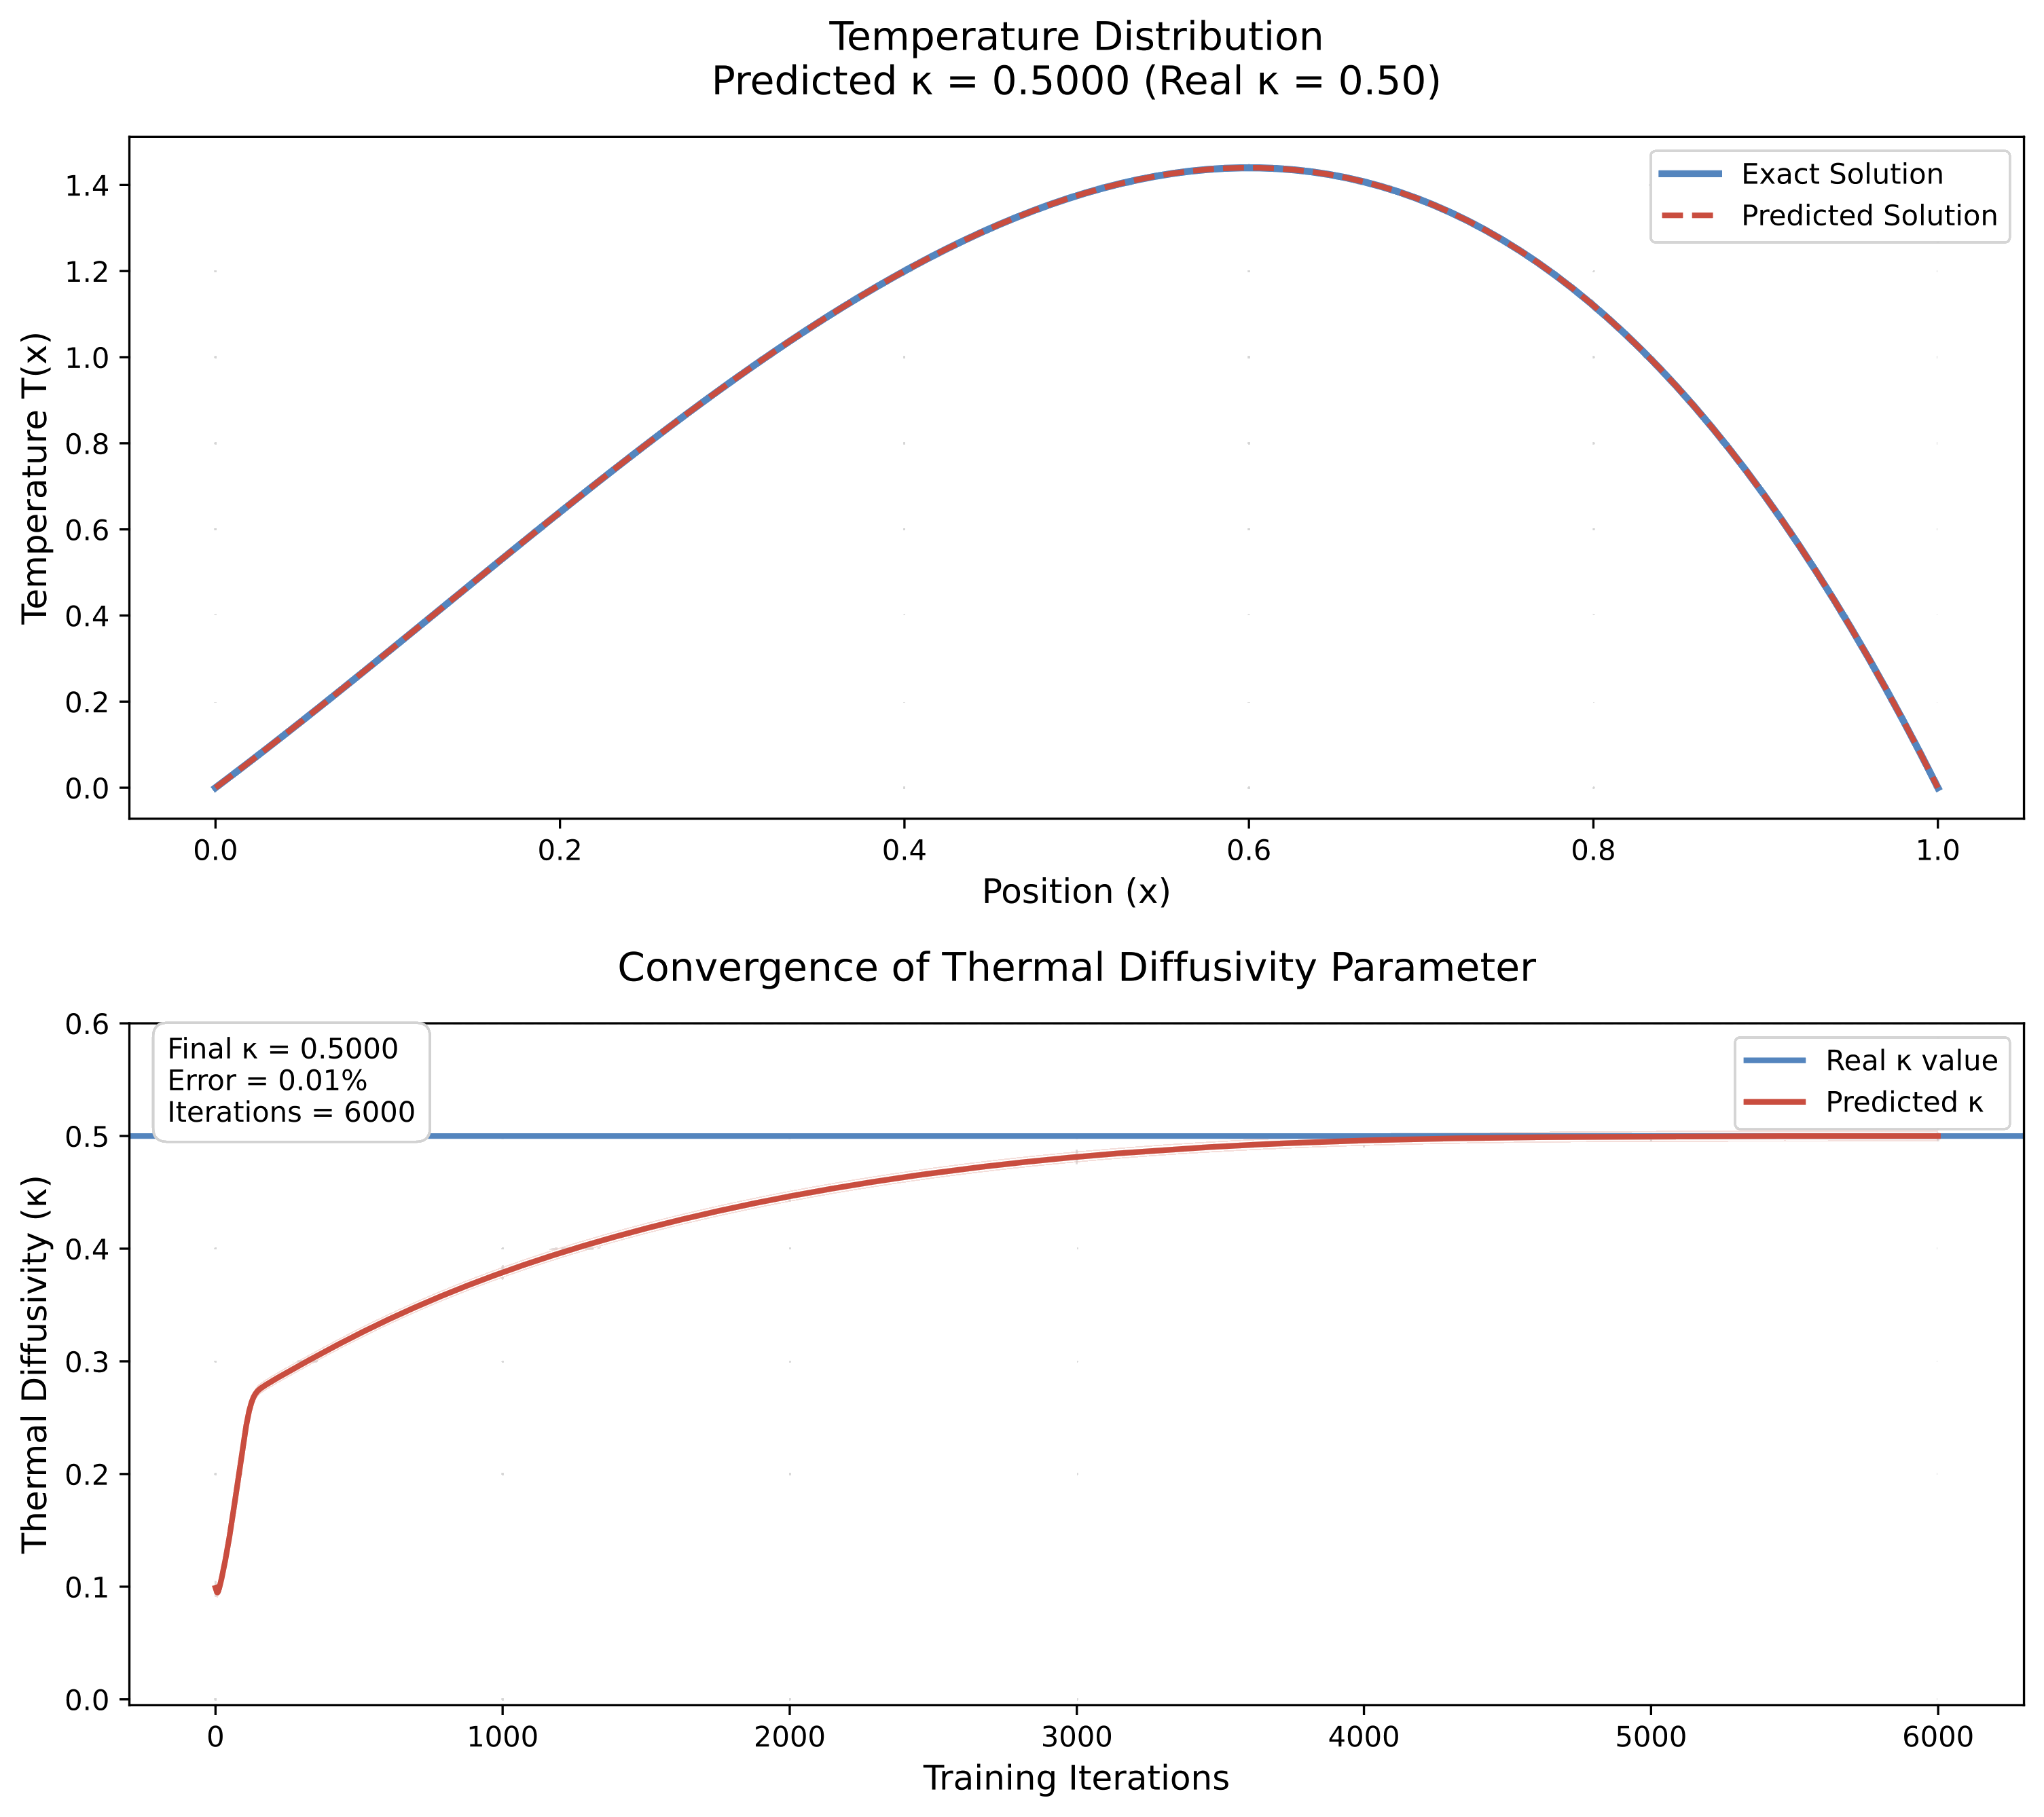
\includegraphics[width=0.8\textwidth]{chapters/04-pinns/figs/inverse-heat-diffusivity.pdf}
\caption{PINN parameter estimation for 1D heat conduction. Top: Predicted temperature profile (blue line) agrees well with sparse measurements (red dots) and the exact solution (dashed line). Bottom: The estimated thermal diffusivity $\kappa$ (blue line) converges accurately to the true value (red dashed line) during training, starting from an initial guess of $\kappa_0=0.1$.}
\label{fig:heat_results}
\end{figure}

As shown in \cref{fig:heat_results}, the PINN successfully recovers both the temperature profile and the unknown diffusivity $\kappa$. Starting from an initial guess $\kappa_0 = 0.1$, the estimated value converges rapidly to the true value $\kappa = 0.5$ with high accuracy (relative error < 0.1\%). This demonstrates the power of using the PDE constraint $\mathcal{L}_{\text{PDE}}$ as regularization; it allows accurate parameter identification even when direct measurement data is very limited and noisy.

\subsection{Example 2: Inferring Burgers' Equation Parameters}

A more challenging inverse problem involves the time-dependent Burgers' equation \eqref{eq:burgers_equation}, where we might want to infer the advection parameter $\lambda_1$ and the viscosity parameter $\lambda_2$:
%
\begin{equation*}
\frac{\partial u}{\partial t} + \lambda_1 u\frac{\partial u}{\partial x} - \lambda_2 \frac{\partial^2 u}{\partial x^2} = 0\,.
\end{equation*}
%
Suppose we have sparse measurements $u_i$ at various space-time locations $(x_i, t_i)$. We want to find $\lambda_1$ and $\lambda_2$.

\notebook[Interactive notebook on inverse parameter estimation for Burgers equation]{https://sciml-book.github.io/sciml_notebook/pinns/burgers.html}

The setup involves:
\begin{itemize}
    \item A neural network $\hat{u}_\theta(x, t; \boldsymbol{\theta})$ approximating the solution $u(x, t)$.
    \item Trainable scalar parameters $\lambda_1$ and $\lambda_2$.
\end{itemize}
The loss function includes terms for data mismatch, the PDE residual (now involving $\lambda_1, \lambda_2$), initial conditions, and boundary conditions:
%
\begin{equation*}
\mathcal{L}(\boldsymbol{\theta}, \lambda_1, \lambda_2) = w_{\text{data}}\mathcal{L}_{\text{data}} + w_{\text{PDE}}\mathcal{L}_{\text{PDE}} + w_{\text{IC}}\mathcal{L}_{\text{IC}} + w_{\text{BC}}\mathcal{L}_{\text{BC}}\,,
\end{equation*}
%
where
%
\begin{align*}
\mathcal{L}_\text{data}(\boldsymbol{\theta}) &= \frac{1}{N_d}\sum_{i=1}^{N_d}|\hat{u}_\theta(x_i, t_i; \boldsymbol{\theta}) - u_i|^2\,, \\
\mathcal{L}_\text{PDE}(\boldsymbol{\theta}, \lambda_1, \lambda_2) &= \frac{1}{N_f}\sum_{j=1}^{N_f}|\frac{\partial \hat{u}_\theta}{\partial t} + \lambda_1 \hat{u}_\theta\frac{\partial \hat{u}_\theta}{\partial x} - \lambda_2 \frac{\partial^2 \hat{u}_\theta}{\partial x^2}|^2_{(x_j^f, t_j^f)}\,, \\
\mathcal{L}_\text{IC}(\boldsymbol{\theta}) &= \frac{1}{N_{ic}}\sum_{k=1}^{N_{ic}}|\hat{u}_\theta(x_k^{ic}, 0; \boldsymbol{\theta}) - u_0(x_k^{ic})|^2\,, \\
\mathcal{L}_\text{BC}(\boldsymbol{\theta}) &= \frac{1}{N_{bc}}\sum_{l=1}^{N_{bc}}(|\hat{u}_\theta(-1, t_l^{bc}; \boldsymbol{\theta})|^2 + |\hat{u}_\theta(1, t_l^{bc}; \boldsymbol{\theta})|^2)\,. % Assuming zero BCs
\end{align*}
%
Training minimizes this loss with respect to $\boldsymbol{\theta}$, $\lambda_1$, and $\lambda_2$. For complex nonlinear problems like Burgers', careful implementation strategies might be needed, such as using different learning rates for network weights versus physical parameters, good initialization, or adaptive sampling near high-gradient regions.

Consider the shock-forming case ($u_0(x) = -\sin(\pi x)$) where the true parameters are $\lambda_1 = 1.0$ and $\lambda_2 = 1/(100\pi) \approx 0.00318$. We use only 1\% of the grid points from a numerical simulation as training data.

\begin{figure}[htbp]
\centering
\includegraphics[width=0.85\textwidth]{chapters/04-pinns/figs/burgers-inverse-prediction.png}
\caption{PINN prediction (dashed lines) versus true solution (solid lines) for Burgers' equation at different times, when parameters $\lambda_1, \lambda_2$ are learned simultaneously from sparse data.}
\label{fig:burgers_inverse}
\end{figure}

\begin{figure}[htbp]
    \centering
    \includegraphics[width=0.85\linewidth]{chapters/04-pinns/figs/burgers-parameter-estimate.pdf}
    \caption{Convergence of the estimated parameters $\lambda_1$ (blue) and $\lambda_2$ (red) towards their true values (dashed lines) during PINN training for the Burgers' equation inverse problem.}
    \label{fig:burgers-parameter-convergence}
\end{figure}

As shown in \cref{fig:burgers_inverse,fig:burgers-parameter-convergence}, the PINN successfully identifies both parameters with high accuracy:
\begin{itemize}
    \item Identified $\lambda_1 \approx 0.973$ (2.7\% error)
    \item Identified $\lambda_2 \approx 0.00318$ (0.6\% error)
\end{itemize}
The predicted solution also matches the true solution well, correctly capturing the shock's position and strength. This demonstrates that PINNs can solve challenging nonlinear inverse problems, inferring multiple physical parameters accurately even from very sparse data, thanks to the strong regularization imposed by the underlying PDE structure. This capability is one of the most compelling features of the physics-informed machine learning approach.


\section{Challenges and Considerations in Training PINNs}
\label{sec:challenges}

Physics-Informed Neural Networks offer a compelling approach to solving differential equations, blending the power of deep learning with the rigor of physical laws. However, successfully training a PINN is not always straightforward. Several challenges can arise, stemming from the nature of the loss function, the optimization process, and the inherent properties of neural networks. Understanding these challenges is crucial for effectively applying PINNs and interpreting their results.

\subsection{The Difficulty of the Loss Landscape: Ill-Conditioning}

The function that a PINN tries to minimize, the loss function $\mathcal{L}(\boldsymbol{\theta})$, often has a complex and challenging "shape" in the high-dimensional space of parameters $\boldsymbol{\theta}$. This landscape combines terms for fitting data (if available), satisfying boundary/initial conditions, and minimizing the PDE residual.

A key difficulty is that this landscape is often \textbf{ill-conditioned}. What does this mean intuitively? Imagine a landscape with extremely steep canyons in some directions but vast, nearly flat plateaus in others.
\begin{itemize}
    \item \textbf{Steep Directions:} Small changes in some parameter combinations cause very large changes in the loss. This corresponds to large eigenvalues of the Hessian matrix (the matrix of second derivatives of the loss). Optimizers might overshoot or oscillate wildly in these directions.
    \item \textbf{Flat Directions:} Large changes in other parameter combinations cause very small changes in the loss. This corresponds to eigenvalues near zero. Optimizers struggle to make progress in these directions, leading to slow convergence.
\end{itemize}
Studies analyzing the Hessian spectrum confirm this picture: a few large outlier eigenvalues and many eigenvalues clustered near zero \cite{krishnapriyan2021characterizing, rathore2024challenges}. This anisotropy makes it difficult for standard gradient-based optimizers to find the minimum efficiently. They might get stuck on saddle points (where the gradient is zero but it's not a minimum) or crawl very slowly across flat regions. The presence of differential operators in the loss terms often contributes significantly to this ill-conditioning.

\subsection{Optimization Challenges: Finding the Minimum}

The ill-conditioned loss landscape directly impacts the performance of the optimization algorithms used to train PINNs.

\paragraph{Standard Optimizers:}
Gradient-based methods like Adam and L-BFGS are common choices.
\begin{itemize}
    \item \textbf{Adam:} A first-order method, generally good at escaping saddle points but can be slow to converge in flat regions or may struggle with the steep directions of ill-conditioned landscapes.
    \item \textbf{L-BFGS:} A quasi-Newton method (using approximate second-derivative information), often converges faster near a minimum by handling local curvature better. However, it can be more easily trapped in local minima or saddle points and can be more computationally expensive per iteration.
\end{itemize}
A common practical strategy is to use Adam initially to navigate the landscape broadly and then switch to L-BFGS for faster convergence near the solution. However, even this hybrid approach may not always be sufficient.

\paragraph{Multi-Objective Nature and Gradient Conflict:}
A unique challenge arises because the PINN loss \eqref{eq:loss_general} is inherently \textbf{multi-objective}. The network tries to satisfy several potentially competing goals simultaneously: minimize the PDE residual, match boundary conditions, match initial conditions, and fit any observation data.

During training, the gradients calculated for each loss component ($\nabla_{\boldsymbol{\theta}}\mathcal{L}_{\text{PDE}}$, $\nabla_{\boldsymbol{\theta}}\mathcal{L}_{\text{BC}}$, etc.) might point in different directions in the parameter space. This is known as \textbf{gradient conflict}. For example, an update that significantly reduces the PDE residual might simultaneously increase the error at the boundary.

This problem is often exacerbated by differences in the magnitudes of the gradients from different terms. Frequently, the gradient from the PDE residual term ($\mathcal{L}_{\text{PDE}}$) is much larger than gradients from boundary or initial conditions \cite{wang2021understanding}. In a simple weighted sum \eqref{eq:loss_general}, the optimizer might prioritize satisfying the PDE in the interior while neglecting the conditions at the boundaries, leading to incorrect solutions. Furthermore, the PDE residual term alone often has many local minima (corresponding to functions that solve the PDE but not the specific boundary/initial value problem), and getting stuck near one of these can prevent the boundary/initial conditions from ever being satisfied \cite{liu2024config}.

\paragraph{Addressing Gradient Conflict:}
Simply adjusting the weights ($w_{\text{PDE}}, w_{\text{BC}}, \dots$) in the loss function is the most common approach but can require extensive tuning. More advanced optimization strategies aim to address gradient conflict directly. Methods like ConFIG (Conflict-Free Inverse Gradients) \cite{liu2024config} and related techniques \cite{yu2020gradient} attempt to find an update direction for the parameters $\boldsymbol{\theta}$ that guarantees improvement (or at least non-worsening) for *all* loss components simultaneously, effectively resolving the conflict. These methods often involve projecting or manipulating the gradients from individual loss terms. While mathematically more involved, they can lead to more robust and reliable training, especially for problems with strong gradient conflicts \cite{liu2024config}. Exploring these advanced optimizers is an active area of research.

\subsection{Spectral Bias: Trouble with High Frequencies}

Neural networks, particularly when trained with standard gradient descent methods, exhibit a phenomenon known as \textbf{spectral bias} \cite{rahaman2019spectral}. They tend to learn low-frequency (smooth) components of the target function much faster and easier than high-frequency (highly detailed or oscillatory) components.

This poses a challenge for PINNs when the true solution to the PDE contains sharp gradients, discontinuities (like shock waves in Burgers' equation), or intricate, high-frequency features (common in turbulence or wave propagation). The network might learn the overall smooth structure of the solution but fail to capture these crucial high-frequency details, even with extensive training or hyperparameter tuning \cite{krishnapriyan2021characterizing}. This can limit the accuracy of PINNs for certain classes of problems, such as convection-dominated flows or reaction-diffusion systems with complex patterns.

\subsection{Mitigation: Curriculum Learning and Sequential Strategies}

To combat some of these training difficulties, researchers have proposed innovative training strategies:

\begin{itemize}
    \item \textbf{Curriculum Regularization:} Start training with a simplified version of the problem or physics (e.g., lower Reynolds number, simpler boundary conditions, larger viscosity) and gradually increase the complexity as the network learns. This guides the network towards the correct solution region before confronting it with the full difficulty of the problem \cite{krishnapriyan2021characterizing}.
    \item \textbf{Sequential Learning:} For time-dependent problems, instead of training over the entire time interval $[0, T]$ at once (as in \cref{sec:continuous_time}), train the network sequentially over smaller time segments. This breaks down the complex task into more manageable pieces and can improve accuracy, especially for long-time simulations or problems with evolving complexity. Domain decomposition in space can achieve similar benefits.
\end{itemize}
These strategies essentially provide a structured learning path for the network, potentially avoiding some of the pitfalls of the complex, non-convex optimization landscape.

\subsection{The Trade-off of Soft Regularization}

Finally, it's important to remember that the standard PINN formulation enforces physics constraints via "soft" regularization – adding penalty terms ($\mathcal{L}_{\text{PDE}}, \mathcal{L}_{\text{BC}}, \dots$) to the loss function. This introduces an inherent trade-off, controlled by the loss weights (like $\lambda$ in \cref{eq:loss_total_pinn} or the $w$'s in \cref{eq:loss_general}).

\begin{itemize}
    \item \textbf{Small Weights:} If the weights for the physics/boundary terms are too small, the optimization landscape might be simpler, but the resulting solution may not accurately satisfy the PDE or boundary conditions. The network prioritizes fitting any available data points.
    \item \textbf{Large Weights:} If the weights are too large, the physics/boundary constraints are emphasized, but this can exacerbate the ill-conditioning of the loss landscape, making optimization much harder \cite{krishnapriyan2021characterizing}. The network might struggle to converge or fit the data points well.
\end{itemize}
Finding the right balance is key and often requires careful tuning for each specific problem. This contrasts with "hard" constraint methods (like the strong enforcement of boundary conditions discussed in \cref{sec:strong_bc}) where constraints are satisfied by construction, potentially simplifying the loss function but requiring more complex network architectures or problem formulations.

In conclusion, while PINNs represent a significant advance, achieving reliable and accurate results requires awareness of these potential challenges related to optimization, function representation (spectral bias), and the balancing of multiple objectives within the loss function. Ongoing research continues to develop more robust network architectures, training strategies, and optimization algorithms to overcome these hurdles.

% --- Problem Set and Notes 

\begin{problemset}[Physics-Informed Neural Networks]

\begin{problem}[1D Steady-State Heat Equation]
Consider the one-dimensional steady-state heat conduction problem with a heat source on a rod of unit length. The governing equation is:

\begin{equation*}
\frac{d^2T}{dx^2} + \frac{q(x)}{\kappa} = 0, \quad x \in [0,1]\,,
\end{equation*}
with homogeneous Dirichlet boundary conditions:
\begin{equation*}
T(0) = T(1) = 0\,.
\end{equation*}
Given a thermal diffusivity constant: $\kappa = 0.5$
and Heat source term: $q(x) = 15x - 2$.\\

\noindent
\begin{enumerate}[a)]

\item Design a physics-informed neural network with:

    \begin{itemize}
    \item Input dimension: 1 (spatial coordinate $x$)
    \item Three hidden layers with 32 neurons each
    \item Hyperbolic tangent activation functions
    \item Output dimension: 1 (temperature $T$)
    \end{itemize}

\item Construct the physics-informed loss function $\mathcal{L}_{Physics}$ that enforces the PDE.

\item Write the boundary loss function $\mathcal{L}_{BCs}$.

\item Train the network using:
    \begin{itemize}
    \item $N_f = 100$ equidistant collocation points
    \item Total loss $\mathcal{L} = \mathcal{L}_{BCs} + \mathcal{L}_{Physics}$
    \item Adam optimizer with learning rate $10^{-3}$
    \item 10,000 epochs
    \end{itemize}

\item Derive the analytical solution and compare it with the numerical solution. Plot both solutions and compute the relative $L^2$ error.
\end{enumerate}

\end{problem}

\begin{problem}[Training Data Study]
Investigate how the number and distribution of collocation points affect solution accuracy:

\begin{enumerate}[a)]
\item Compare uniform vs. random sampling of collocation points
\item Study convergence for $N_f = \{50, 100, 200, 500\}$ points
\item Analyze the trade-off between the number of points and training time
\item Recommend an optimal sampling strategy
\end{enumerate}

\end{problem}

\begin{problem}[Architecture Analysis]
Study how the neural network architecture impacts performance:

\begin{enumerate}[a)]
\item Compare networks with different depths (2, 3, 4 layers)
\item Analyze the effect of width (16, 32, 64 neurons per layer)
\item Test different activation functions (tanh, ReLU, sigmoid)
\item Justify your final architecture choice with quantitative evidence
\end{enumerate}

\end{problem}

\begin{problem}[Loss Function Design]
Investigate different formulations of the loss function:

\begin{enumerate}[a)]
\item Implement adaptive loss weighting:
    \begin{equation*}
    \mathcal{L} = \alpha(t)\mathcal{L}_{BCs} + \beta(t)\mathcal{L}_{Physics}
    \end{equation*}
    where $\alpha(t)$ and $\beta(t)$ are dynamic weights.

\item Compare with the original fixed-weight formulation

\item Study the impact of different weight schedules:
    \begin{itemize}
    \item Constant weights
    \item Linear annealing
    \item Exponential decay
    \end{itemize}

\item Propose and justify an optimal weighting strategy
\end{enumerate}

\end{problem}

\begin{problem}[Variational Formulation]
Implement and analyze a variational (weak) form of the problem:

\begin{enumerate}[a)]
\item Derive the weak form by multiplying the PDE by test functions $\phi(x)$ and integrating:
    \begin{equation*}
    \int_0^1 \frac{dT}{dx}\frac{d\phi}{dx}dx = \int_0^1 \frac{q(x)}{\kappa}\phi dx
    \end{equation*}

\item Implement this formulation using neural networks

\item Compare with the strong form implementation in terms of:
    \begin{itemize}
    \item Solution accuracy
    \item Training stability
    \item Computational efficiency 
    \end{itemize}

\item Discuss the advantages and disadvantages of each approach
\end{enumerate}

\end{problem}

\begin{problem}[Advanced Extensions]
Choose one of the following extensions:

\begin{enumerate}[a)]
\item Implement a nonlinear diffusion coefficient:
    \begin{equation*}
    \kappa(T) = \kappa_0(1 + \alpha T)
    \end{equation*}

\item Add a convection term:
    \begin{equation*}
    \frac{d^2T}{dx^2} + v\frac{dT}{dx} + \frac{q(x)}{\kappa} = 0
    \end{equation*}

\item Solve the time-dependent version:
    \begin{equation*}
    \frac{\partial T}{\partial t} = \kappa\frac{\partial^2 T}{\partial x^2} + q(x)
    \end{equation*}
\end{enumerate}

Analyze how your chosen extension affects the PINN implementation and performance.
\end{problem}

\begin{problem}[Data-Driven Cross-Section Identification]
Consider the static bar equation where the displacement field $u(x)$ is known but the cross-sectional properties $EA(x)$ need to be identified:

\begin{equation*}
\frac{d}{dx}(EA(x)\frac{du}{dx}) + p(x) = 0, \quad x \in [0,1]
\end{equation*}

Given:
\begin{itemize}
\item Displacement field: $u(x) = \sin(2\pi x)$
\item Distributed load: $p(x) = -2(3x^2 - 2x)\pi \cos(2\pi x) + 4(x^3 - x^2 + 1)\pi^2 \sin(2\pi x)$
\item Domain: $x \in [0,1]$
\item Boundary conditions: $u(0) = u(1) = 0$
\end{itemize}

\begin{enumerate}[a)]
\item Design a physics-informed neural network to identify $EA(x)$ with:
    \begin{itemize}
    \item Input dimensions: 2 (spatial coordinate $x$ and displacement $u$)
    \item Three hidden layers with 20 neurons each
    \item Hyperbolic tangent activation functions
    \item Output dimension: 1 (stiffness $EA$)
    \end{itemize}

\item Formulate the physics-informed loss function that enforces the differential equation.

\item Train the network using:
    \begin{itemize}
    \item $N = 100$ uniformly distributed training points
    \item Adam optimizer with learning rate $10^{-3}$
    \item 5,000 epochs
    \end{itemize}

\item Compare the identified $EA(x)$ with the analytical solution:
    \begin{equation*}
    EA(x) = x^3 - x^2 + 1
    \end{equation*}

\item Study the influence of noise in the displacement measurements by adding Gaussian noise with different standard deviations:
    $\sigma = \{0.01, 0.05, 0.1\}$.
\end{enumerate}

\end{problem}

\end{problemset}   


\notes{
Key points to consider while solving these problems:
\begin{itemize}
\item Use automatic differentiation for computing derivatives
\item Monitor both physics and boundary losses during training
\item Save models at different epochs to analyze the convergence
\item Document all hyperparameters and architectural choices
\item Validate the prediction against the exact solution (e.g., $T(x)=−5x^3 +2x^2 +3x$ for Problem 1.1)
\end{itemize}
}